\setcounter{chapter}{3}
\chapter{kelavu ASaR shabadxgaLa aMtaraMgate}

(shirxVmanamxhArAja jayacAmarAjeVMdarx oDeyarf avaru shirxVmAnf ke. esf. varadAcArayxru matutx shirxVmAnf enf. esf. veMkaTanAthAcArayxravara mUlaka, kelavu AdhAyxtimxka keSxVtarxkekx saMbaMdhisida padagaLanunx gurutisi avugaLa bagegx vivaraNeyanunx keVLidaru, A vicAravanunx shirxV shirxVraMga mahAguruvinalilx niveVdisidAga avara saluvAgi ivaribabxrigU koTuTx anugarxhisida pAThagaLu)

saMgArxhakaru shirxV enf. esf. vi. avaru.

(pAThadalilx upasithxtarAgidadxvaru - shirxV ke. esf. vi. matutx enf. esf. vi.)

\noindent
{\bf\large{parxtipAdayx viSayAnuguNavAda deVvatA sutxti}}\label{page128}

(shirxVguruvu savxlapxhotutx dhAyxnArUDarAgidudx, naMtara aMjali baMdhadoDane - I keLakaMDa sholxVkagaLanunx gAnamADidaru)

\begin{description}
\item[(1)] vishovxVtitxVNaR savxrUpAya cinamxyAnaMdarUpiNeV |\label{128}
\item  tuBayxM namoV hayagirxVva vidAyxrAjAya viSaNxveV ||
\item[(2)] namasetxV cidacidavxgaRsaMrakaSxNavicakaSxNeV|\label{128}
\item  jagadivxdhAnashilipxnenxY viSuNxpatenxY namoV\char'263sutx teV||
\end{description}

viSaya parxtipAdanege anuguNavAda ASaRvacana
\begin{description}
\item[(3)] asheVSadaqshoyxVjiGxta daqknmxyAnAM avasithxtAnAmiha rAjayoVgeV|\label{128}
\item  na jAgaroV neYSa suSupitxBAvoV na jiVvitaM noV maraNaM vicitarxmf ||
\item[(4)] UdhavxRmUlamadhashAyxKaM ashavxtathxM pArxhuravayxyamf |\label{128}
\item  CaMdAMsi yasayx paNARni yasatxM veVda sa veVdavitf ||
\end{description}

\noindent
{\bf\large{jagadAcArayxnAda hayavadanadiMda vANige ceYtanayx}}\label{page128}

beLavaNigeyalilx horaTiruva I jiVvana vaqkaSxkekx oMdu mUlavuMTu. jiVvana vaqkaSxkekx mUlavAdayAva vasutxvuMToV, adeV vidAyxmUlavU, nAda-shariVriyU Ada joyxVtiyAgideyapApx! I jiVvana vaqkaSxda joteyalelxV jAcnxna vaqkaSxvanUnx beLesabeVkAgide. oMdu biVjavanunx keSxVtarxdalilx neTuTx pAlaneyoMdige adanunx beLesikoMDu horaTAga, aMkura modalugoMDu ciguru, koMbe-reMbegaLu, hUvu, miDi, kAyi, haNuNx ivugaLalilx parxtiyoMdu aMshakUkx heVge oMdu muLakAraNavuMToV, A mUlavanAnxsharxyisikoMDu horaTAga mAtarxveV adu soMpAgi beLeyuvudu sAdhayxvoV, hAgeyeV vidAyxsaMbaMdhavAgi yAvudeV oMdu mAtu horaTAgalU, adakUkx mUlavoMdiruvudu. A joyxVtiVrUpavAda mUlavoMdilalxdAdAga I mAtU saha satayxvU suMdaravU Agi beLeyalAradu.

UdhaRvx mUlavAgiruva idU, A mUladiMda tanage beVkAdadxnunx tegedukoMDu I iMdirxya rUpavAda shAKoVpashAKegaLoDane soMpAgi beLeyabeVkAda jiVvanavAgide. idaralUlx vAknUmxlavAgi horaDuva mAteMbudu, adara mUlavanenxV muTaTxdeV horaDuvudAdare adaralilx satavxviruvudilalxdAgutetx. aMteyeV swMdayaRyukatxvAda beLavaNige iruvudilalx.

\noindent
{\bf\large{`aMkeVnoVdUhayx vAgedxVviVmAcAyaRkamupAshirxtaH'}}

eMbaMte yAva hayavadananu, tananx maDilalilx vAgedxVviyanunx kuLiLxrisikoMDu, jAcnxnamuderxyoDane tananxdeV Ada AnaMdadhAmadalilx kuLitu, jagadAcAyaRnAgi beLaguvanoV, A nananx sAvxmiyanunx samxrisikoMDu, avaniMdaleV nananx I vANige ceYtanayxvanunx tuMbisikoMDu, nimamx muMde adaninxDuvavanAgidedxVneVpapx!

\noindent
{\bf\large{I deVhavu nashavxravAdarU amara BAvavanunx horatarabalalx sAdhanavU Agide}}\label{page129}

parxkaqti maMDalakekx silukida parxtiyoMdu vasutxvinalUlx sahajavAgiyeV maraBAvavu (nashavxrate) iruvudAgide. maraBAvaveV parxparxthamavAgi edudx kANuvudU Agide. Adare videyxya matutx kaleya mUlaka alilxruva I aMshavanunx maretu adara hiMbadiyalilxruva amara BAvavanunx adaralilxratakakx satayx-swMdarayx-mAMgalayxgaLanUnx kANabeVkAgide. avugaLaninxdaralilx kaMDu adariMda namamx jiVvanadalUlx swMdarayxvanUnx taMdukoLaLxbeVku. maraBAvadalilxruva idU A amaratavxvanunx samxrisikoMDu horaTAga amaravAgiyeV kaMDu maraBAva matutx amara BAva eraDU oMdeDe hoMdANikeyiMdiruvudanunx nAvu noVDalu sAdhayxvAgutatxde. udAharaNege- idoMdu taMbUri, idakekx baLasiruva maravanunx tegedukoMDu koDaliya kAvAgiyU mADabahudu, gudadxliya kAvAgiyU mADabahudu, maNeyAgiyU mADabahudu, hiDigaLanUnx mADabahudu, kaLaLxnanunx hoDedoVDisuva oMdu doNeNxyAgiyU mADabahudu. I heVLida rUpagaLelalxvU adaralilxya maraBAvada visAtxraveV Agide. Adare idanenxV obabx kalAkArana keYyalilx koTATxga avanu adanunx tegedukoMDu I rUpakekx (taMbUriya) taMdu, nAdada rahasayxvananxritu, I riVti guMBitavAgi taMtiya mUlaka nAdavu horaDuvaMte mADi, A nAdadalilx parxNavaGoVSavu parxtibiMbitavAgi amaraBAvadeDege jiVviya manasasxnunx oyuyxva oMdu sAdhanavAgi adaralilx sahajavAgidadx maratavxvanunx mareyisi, amaraBAvavanunx taMdukoDuva kalAkaqtiyAgi idanunx mADutAtxne. hAgeyeV (tamamx deVhada kaDege keY toVrisi). oMdu jaDavasutxveV AdarU avana sAninxdhayxdiMda, avana kaleyiMda cinamxyavAgi avana oMdu dhavxniyanUnx, avanadeV Ada nAdavanUnx horasUsalu kAraNavAdaMtaha vasutxvAgideVpApx.

\noindent
{\bf\large{oLanAdavanunx horataralu deVhakokxMdu saMsAkxravirabeVku}}\label{page130}

nAdaveMbudu nitayx matutx amara. adu QuSigaLa haqdayAMtarALadalilx iruvaMtadu. adanunx I BwtikavasutxgaLa mUlaka horapaDisalu yatinxsidAga adakakxnuguNavAgidadxre athavA iTuTxkoMDidadxre mAtarx amaraBAvavanunx taLedu, A QuSigaLa haqdayAMtarALadalilxdadx nAdavanenxV horatarutatxde. oMdu hUvinoMdige, samanasadoMdige nArU saha savxgaRkekx hoVguvaMte (hArada rUpavanunx hoMdi BagavaMtana kaMThadalilx viharisuvaMte) I sumanasisxnoMdige I naranU nArAyaNana saninxdhige talupavaMte AgideVpApx.

\noindent
{\bf\large{parxsutxtagoLisutitxruva viSayagaLu aMtaraMgada parxBuvina parxsAda rUpavAgive.}}

I muMde heVLuva viSayagaLu maravAda nananx bAyiya mUlaka horapaDuvudAgidadxrU adaralilx toVruva viSayagaLanunx keVvala nimamx muMdiruva vayxkitxya daqSiTxyiMdaleV noVDade, adakUkx mUlavAda amaraBAvadiMda barutitxruvudAgi noVDipApx. vayxkitxyu eMdAdaromemx mareyAgabahudAdarU, vayxkitxya hiMdiruva vayxkitxtavxkekx mUlavAda shakitxyu mAtarx eMdU mareyAguvaMthadalalxveMbudanunx mareyadiriVpApx. I nimamxlilxDuva viSayavu nimamx daqSiTxyiMda horagaDeya rAjanige iDuvudakokxVsakxraveMdu niVvu keVLutitxdadxrU nAnu mAtarx yAvanu nananx aMtaraMgadalilx rAjanAgiyU, savxrATf AgiyU, virATf AgiyU beLagutitxruvanoV A parxBuvina pAdamUladalilx apiRsi, avana parxsAdavAgi paDedu, naMtara nimamx muMde iDuvavanAgidedxVne.

\noindent
{\bf\large{modalige haqdayakekx viSaya naMtara itararige tiLisuva vicAra}}\label{page131}

niVvu maMdiradavarAgi kuLitu I viSayavanunx sariyAgi manasisxge taMdukoLiLx. adara naMtara horagaDeya nimamx rAjana muMdiDalu javAbAdxri, deVsha-kAlagaLu, parxkaqti-saninxveVshagaLu elalxvanUnx aritu iDuviraMte. avaru keVLiruva parxshenxgaLige avariMdaleV eSuTx aBipArxyavanunx paDeyabeVku, naMtara eSuTx utatxravanunx vAyxvahArikavAgiDabeVku, kataRvayxdaqSiTxyiMda utatxradalilx eSuTx viSayaviDabeVku, adaralilx yAva riVti-niVtigaLanunx anusarisabeVku anunxvudara bagegx kelavu mAtugaLanunx ADabeVkAgide. paraMtu parxshenxyaninxTaTx avarige oMdu riVtiyalilx viSayagaLanunx koDuvudu ucitaveMdu kaMDubaMdadariMda adanunx pATharUpAvAgi nimamxlilxDuvavanAgidedxVne. modalige nimamx manasisxge sariyAgi tegedukoLiLx. avarige iDuvudu naMtarada vicAra.

\noindent
{\bf\large{viSaya nirUpaNeyalilx karxma}}

niVvu hiMdekoTaTx kAgadada parxkAra kaMDubaMdaMtaha viSayagaLanunx koVshagaLalilx ({\rm dictionary}) huDukalu anukUlavAgaleMdu akArAdi karxmadalilx avugaLanunx gurutu hAkidedxVne. (avanu gurutu hAkida karxmadalilx Odi toVrisidaru.) iSuTx viSayagaLa bagegx viSayAnuguNavAgi matutx swlaBayxda daqSiTxyiMda modaladinavAda iMdu odaguvaSuTx kAlAvakAshakekx takakxMte nADada bagegx kelavu vicAragaLanunx iDuvavanAgidedxVne.

\noindent
{\bf\large{mahArAjara parxshenxge utatxrisalu agatayxvAda sidadhxte hAgu javAbAdxri}}\label{page131}

I bagegx avaru veVda, upaniSatutx, purANa matutx kAvayx-ivugaLelalxdara meVlU saveRmADi adara sArAMshavanunx bareyabeVkeMdu keVLidAdxre. avaru koTiTxruva kAlAvakAsha hadineYdu dinagaLu mAtarx. saveRmADabeVkAda garxMthagaLa daqSiTxyiMda noVDidAga eSoTxV tiMgaLugaLa kAla beVkAgutatxde. I vicAradalilx oMdu sAmAnayxvAda aiDiyA AdarU beVku. yAvudeV daqSiTxyanUnx harisade keVvala shabadxpArAyaNavAgi rAmAyaNavanunx Odi mugisalu oMBatutx dinagaLanunx (navarAtirxyalilx) iTiTxdAdxre. hiVgiruvAga sUkaSxmXdaqSiTxyiMda ivelalxvanUnx gamanisikoMDu mugisalu bahaLa kAlAvakAshabeVkeMba viSayavanunx avarige tiLisabeVkAgide. AdadxriMda koDabeVkAda utatxravanunx oMdu saMgarxharUpavAgi koTuTxkoLiLx. oMdu veVLe mahArAjadiMda parxshenx baradeV idadxrU niVvAgiyeV maMdirada mUlakavAgi parxshAnxvakAshavanunx iTuTxkoMDu I bagegx pAThavanunx garxhisi, naMtara viSayagAMBiVrAyxnuguNavAgi iDuvaMte mADikoLiLx.

\noindent
{\bf\large{veVdaveMdarAvudu?}}\label{page132}

parxkaqta viSayagaLanunx veVdagaLalilx huDukabeVku eMdAga alilx huDukalu yatinxsuva munanx, veVdaveMdareVnu? A padada padAthaRvAvudu? eMbudara bagegx nishicxtavAda tiLuvaLike beVku. hosa tiLuvaLike Eke? nAlukx veVdagaLu parxsidadhxvAgive, yajuveVRdadalUlx ashiVtidavxyavu elalxra baLakeyalUlx ideyalalx? eMba parxshenx barabahudAdarU iMdu kANutitxruva veVdagaLaSeTxV veVdagaLalalx. EkeMdare-

\begin{shloka}
`na veVdaM veVdamitAyxhuH veVdeV veVdoV na vidayxteV |\\\label{132}
parAtAmx viMdateV yeVna sa veVdoV veVda ucayxteV ||'
\end{shloka}

(aritavaru veVdaveMdu saMkeVtasidadhxvAda shabadxrAshiyanunx veVdavenanxlAraru. veVdadalilx veVdaviruvudilalx. yAvudariMda paramAtamxna lABavAgutotxV aMtaha veVdavu tAneV veVdavenanxlapxDutatxde.) loVkavayxvahAradalilx `oMdu teMginakAyiyanunx tegedukoLiLx' eMdAga maTeTx, juMgu, karaTa, ivelalxdaroMdige iruva padAthaRvanunx tegedukoLuLxtAtxre. aSaTxnUnx seVrisiyeV `kAyi' anunxvudu. Adare aSaTxkUkx seVri `kAyi' eMba vayxvahAravidadxrU oMdu cUru juMganunx tegedukoTaTxre adanunx `kAyi' eMdu yArU opipxkoLuLxvudilalx. EkeMdare vasutxtaH oLagiruva tiruLeV kAyi. adanunx daqSiTxyalilxTuTx, oLaginadadxnunx mareyade, adara horagina AvaraNakekxlAlx adaroMdige idAdxga `kAyi' eMba vayxvahAra baruvudu. hAgeyeV aMtadaqRSiTxge viSayavAda veVdashabadxvAcayxvAda oMdu vasutxvinoMdige hoMdikoMDu I goragina AvaranavU idAdxga mAtarx aMtaHsAravanunx mareyadeV elalxkUkx seVri veVdaveMba vayxvahAravu barutatxde. hAgilalxde tiruLanunx kaLedukoMDidAdxga keVvala karaTa, juMgugaLaMte I shabadxrAshiyU veVdavenisikoLaLxlu avakAshavilalx.

\noindent
{\bf\large{veVdavidanu yAru?}}\label{page133}

AdadxriMdaleV `veVdavitf' yArU? eMdu nivaRcanamADuvAga, jAcnxnigaLu ``iSuTx adhAyxyavoV, iSuTx maMDalavoV, iSuTx kAMDavoV kalitavanu" eMba vivaraNeyanunx koDade-

\begin{shloka}
jAcnxninAM UdhaRvxgoV BUyAtf ajAcnxniVnAMtavxdhoVmuKaH |\\\label{133}
EvaM veY parxNavasitxSeThxVtf yasatxM veVda sa veVdavitf ||'
\end{shloka}

eMdu heVLidAdxre. (parxNavaveMbudu jAcnxnigaLa deVhadalilx UdhaRvxgati uLaLxdAdxgiyU, ajAcnxnigaLa deVhadalilx adhoVgatiyuLaLxdAdxgiyU (keLamuKavAda harivu) irutatxde. adara (parxNavada) neYjasavxrUpavanunx yAru aritavanoV avaneV veVdavitf, (veVdaveVtatxnu))

\noindent
{\bf\large{veVdavu nitayxveMdareVnu?}}\label{page133}

mahABAratadalilx veVdagaLa arivina bagegx vivaraNe koDutAtx,-

\begin{shloka}
`veVdAMshacx veVdayxM ca vidhiMca kaqtasxnXM athoV nirukatxM paramAthaRtAM ca |\\\label{133}
savaRM shariVrAtamxni yaH parxveVda tasayx samx deVvAH sapxqhayaMti nitayxmf ||'
\end{shloka}

(yAvanobabxnu veVdagaLanUnx, veVdayxvAda tatatxvXgaLanUnx, vidhiyelalxvanUnx aMteyeV paramAthaRvanUnx avayxkatxrUpadalilx tananx shariVrada aMtaraMgadalilx kaMDukoLuLxvanoV aMthavana bagegx deVvategaLU saha iSaTxpaDuvaru.) aMdare `yAvana aMtadaqRSiTxgU, aMtaHsharxvaNakUkx, veVda-veVdayx-vidhigaLelalxvU tananx shariVrAMtaraMgadalilx goVcaravAgududoV avaneV jAcnxni. aMthavanige tAne deYvavU oliyuvudu,' eMdu heVLide. hiVgalalxde namamx baLakeyalilxruva veVdavu mAtarxveV veVdavenisuvudAdare veVda heVLuvavaru horaTuhoVdare veVdaveV horaTuhodaMte AdiVtu. deVshadalilx odaguva nAnA bageya vipalxvagaLiMda veVda pusatxkagaLelalxvU nAshavAgibiTaTxre veVdagaLelAlx nAshavAdaMte AdiVtu. Adare saMparxdAyadavaru veVdavu `nitayx' enunxtAtxre. adu nitayx eMbudu nijavAdare hALAgalu athavA horaTuhoVgalu sAdhayxvilalx. AdadxriMda nitayxvAda veVdavU iMdu jana heVLuva riVtiyalilx iruvudilalx. iMtaha veVdavU iruva jAga yAvudu? eMdare giVteyalilx-

\begin{shloka}
`yoV\char'263MtaHsuKoV\char'263MtarArAmaH tathAMtajoyxVRtireVva yaH ||'\\\label{134}
sa yoVgiV barxhamxnivARNaM barxhamxBUtoV\char'263dhigacaCxti ||' (Ba. giV)
\end{shloka}

(yAvanobabx sAdhakanAdavanu bAheyxVMdirxya matutx bAhayx viSayagaLanunx tananx nemamxdigAgi arasade oLageyeV nemamxdi paDeyabalalx sithxtige talupi, alelx tanamxyiVBAvadiMda ramisuvaMte AguvanoV, yAva Asithxtiyu oLabAgilanunx teredu teVjoVmayavAda aMtaH parxpaMcavanunx dashaRnamADisuvudoV-aMtaha AtamxyoVgavanunx paDedavanu tiroVhitavAgidadx shudadhxbarxhamxBAvavanunx matetx kaMDukoMDu barxhamxtatatxvX rUpavAda moVkaSxvanenxV hoMduvanu.) eMdu heVLide. jAcnxnigaLa aMtaraMgadalilx veVdapuruSaniruvanu. avananunx tiLisuva sAhitayxrUpavAda veVdavU alelxV iruvudu. adu eMdeMdigU nitayx. EkeMdare adara vAcayxvu nitayxvAda meVle adara vAcakavU nitayxveV. avana nitayxvAda BAvavanunx horakekx vayxkatxpaDisalu avanige aMgavAgi horabaMda vANiyu tAneV veVdavANiyAyitu. aMgiyu aMtaraMgadalilxdadxre avanige oMdu aMga. `matotxMdu upAMga. AdadxriMdaleV' `sAMgoVpAMgavAda veVda' anunxva mAtu.

\noindent
{\bf\large{iMdu upalabadhxviruvudaSeTxV veVdavalalx}}\label{page134}

manasisxnalilx oMdu aBipArxyavu udayisidare adanunx horakekx taralu, I (keY)aMgavu sAdhanavAgide. `niVvu ililxge barabeVku, ililx hatitxra, kuLitukoLaLxbeVku.' eMbudAgi oLa BAvavanunx horapaDisuva oMdu BASe huTiTxkoMDare oLagina BAvakekx BASeyu aMgavAgutatxde. keY sanenxya mUlaka horagaDahidAga keYyeV aMgavAgutatxde. oLage yAva aBipArxyavU ilalxdidadxre BASeyAgaliV, keYyAgaliV yAvudakekx aMgavAdiVtu? I riVti oLagina veVdapuruSananunx vayxkatxpaDisalu tAneV veVda, upaveVda matutx upaniSatutx itAyxdigaLelAlx horaTavu. AdadxriMda Iga kAnuva veVda sAhitayx BAgadalelxV elAlx viSayavu sigabeVkeMdare adu asAdhayxvAda viSaya. hiMdidadx eSoTxV veVdaBAgagaLu lupatxvAgiruvudanunx nAvu parxmANaBUtavAda vAkayxgaLiMdaleV tiLiyutatxve.

\noindent
{\bf\large{veVdavanunx adara mUla neleyiMda paDedukoLaLxbeVku}}\label{page135}

`EkashataM adhavxyuRshAKAH sahasarxM sAmashAKAH' |\label{135} eMdelAlx vAkarxgaLive. Iga namage nUreMdu yajuH shAKegaLAgaliV, sAvira sAmashAKegaLAgaliV upalabadhxvAgutilalx. aMteyeV `QugevxVda pArxtishAKayxvu laMDanf leYbarxriyalilx sikikxkoMDide,' itAyxdi vayxvahAravU uMTu. AdadxriMda AdhAragaLanunx veVdagaLalilx huDukalu horaTAga A veVda BAgagaLu namamx deVshadalilxyeV ilalxdidadxre huDukuvudAdarU heVge? AdadxriMda bahukAladiMda beLediruva mwDhayxvanunx toredu, vicAraparatege manasasxnunx koTuTxkoLaLxbeVku. I mAtu veVdavu aparxmANaveMdeVnU tiLisuvudalalx. veVdada nele yAvudoV alelxV adanunx tegedukoMDare adu parxmANavAgabahudeV horatu beVreDe aledADalu horaTare adu parxmANavalalx, BarxmeyalelxV nilulxtatxde, eMbudanunx tiLisalu I mAtu.

\noindent
{\bf\large{parxme, parxmANa hAgU Apatx}}\label{page135}

oMdu viSayakekx parxmANaBUtavAda vacanagaLanunx huDuki paDeyabeVkeMdAga parxmANa shabadxdalilxruva `parxme' eMbudu yAvudoV adu arivAgabeVku. adananxrita meVle adara bagegx huTiTxkoLuLxva vacanavu parxmANavacanavu. aMtaha parxmANavacanavanAnxDuvavareV `Apatx'renisuvaru. avara mAteV ApatxvAkayx. Apatxra lakaSxNavanunx I riVti heVLidAdxre-

\begin{shloka}
`rajasatxmoVBAyxM nimuRkAtxH tapoVjAcnxnabaleVna yeV|\\\label{135}
yeVSAM tirxkAlamamalaM jAcnxnamavAyxhataM sadA ||'\\
`ApAtxshiyxSATx vibudAdhxsetxV teVSAM vAkayxmasaMshayaM |\\
satayxM vakaSxyXMti, teV kasAmxtf asatayxM niVrajasatxmAH ? ||' eMbudAgi.
\end{shloka}

(yAru tapasusx matutx jAcnxnagaLa baladiMda rajoVguNa matutx tamoVguNagaLiMda biDugaDe hoMdiruvaroV, yArige kAlatarxyadalULx taDeyilalxde nimaRlavAda jAcnxnavu iruvudoV aMtaha visheVSavAda boVdhavanunx paDeda shiSaTxreV Apatxru. aMthavara vAkayxvu nisasxMdeVhavAgi satayxvu. rajasatxmoVguNagaLa bAdheyanunx dATida avaru Eke tAne asatayxvanunx heVLiyAru?)

\noindent
{\bf\large{yAvudu parxmANa?}}\label{page134}

yAva jAgadalilx yAva kirxyeyu yAva riVti naDeyuvudoV A viSayakekx adeV parxmANa. A parxmANavaninxTuTxkoMDeV vayxvahAradalilx pArxmANIkateyu itayxthaRvAgabeVku. naDediruva I vayxvahArakekx adanunx citirxsuva rekADuR keVvala oMdu sAkiSxyaSeTxV. (adu sAhitayx rUpavAgabahudu, citarx rUpavAgabahudu athavA shilapxrUpavAgabahudu.)

udAharaNege obabxnu matotxbabxnige oMdu nUrurUpAyigaLanunx sAlavAgi koDutAtxne eMdukoLoLxVNa. A koTaTxvanu sAlapaDeyuvaniMda patarxvanunx bareyisikoLuLxtAtxne athavA oMdu DeYriyalolxV, goVDeyalolxV gurutu hAkikoLuLxtAtxne. AvAga `nA nUrurUpAyi koTiTxdedxVne' eMdu avanedurige bareyutAtxne. naMtara avanu horaTu hoVdameVle guTATxgi adaralilx keYvADa naDesi, `nA' eMbudara muMde `nU' eMbudara keLage otatxkaSxravAda na kAravanunx seVrisi, modalu baredudadxnunx tididx, `nAnUnxrurUpAyi koTiTxdedxVne' eMdu mADibiTaTxre, koVTiRge hoVdAga ivanu tididxruvudU seVri adu parxmANavAguvudAdare `nAnu nUru rUpAyigaLanunx koTiTxdedxVne' eMbudu hoVgi, `nAlukxnUru rUpAyigaLanunx koTiTxdedxVne' eMdu vAyxKAyxnisuvaMtAdAga A munUnxru rUpAyina moVsavu pArxmANikategeV seVribiDabahudu. athavA `nAnUnxru' eMdu baredidadxralilx `nA' otatxnunx guTATxgi aLisi `nAnu nUru rUpAyiyanunx koTiTxdedxVne' eMdu haNa paDedavanu tididxbiTaTxre, adeV parxmANavAdare koTaTxvanige munUnxrUpAyi moVsavAguvudU pArxmANikavAdiVtu. aMtha samayadalilx koTaTxvanAgaliV, paDedavanAgaliV, moVsakokxLagAgadeV irabeVkAdare aMdu naDeda GaTaneyanenxV muMdina vayxvahArakekx parxmANavAgiTuTxkoMDu, naMtara naDeda `poVjaRri'yanunx aparxmANa eMdu GoVSisabeVkAgutatxde. adakekx ibabxrU oDaMbaTaTxre alilx pArxmANikate ilalxdidadxre parxmANaveV beVre, vayxvahAraveV beVre eMdAdiVtu. hAgAguvudAdare gurutu hAkidedxVke? naDe GaTanege gurutu sAkiSxyAguvudu hoVgi moVsakekx AdhAravAdaMte Agutetx. AdadxriMda veVdashAsAtxrXdigaLu parxmANaBUtavAda viSayakekx sAkiSx mAtarxveV horatu adeV orijinalf parxmANavalalx. EkeMdare muMde baMdavaru asAvadhAnateyiMdaloV, citatxBarxmaNeyiMdaloV, otatxkaSxravanunx seVrisuvudoV, idadx otatxkaSxravanunx tegeyuvudoV mADibiTATxga viSayada neYjategU, parxmANaveMdu naMbuva sAhitayxkUkx saMbaMdhavilalxde aDADxDabeVkAdiVtu. AdadxriMda parxmANavu yAvudu? eMbudara bagegx ALavAgi ciMtisi, oMdu niluvige barabeVkAguvudu.

\noindent
{\bf\large{jAcnxna rUpavAda veVdakekx gurutAgidadxre mAtarx sAhitayxrUpavAda veVdavu parxmANa}}\label{page137}

QuSigaLa haqdayadalilx eMdoV oMdu dina naDeda samAcAravanunx avarige sAdhayxvAdaSaTxramaTiTxge liKita mUlakavAgi taruva parxyatanx naDedadudxMTu. adara saluvAgi avu pusatxkarUpeVNa barutitxve. A pusatxkagaLanunx Odi athaRmADikoLaLxlu horaTavaru taMtamamx niluvige takakxMte tirugisuva saMBavagaLuMTu. udAharaNege `tatasxvituvaRreVNayxM' eMbudanunx keVLikoMDu alilx tatasx eMbudanunx matasxyX irabeVku eMdu BAvisikoMDu idu matAsxyXvatArakekx saMbaMdhapaTaTxdudx eMdu Barxmisi, `matasxyXvituvaRreVNayxM' eMdu tidudxvavarU irabahudu. AdadxriMda I sAhitayxvanenxV nimamx parxmANasavaRsavxveMdu BAvisi hejejxyiDabeVDi. aMteyeV yAroV obabxru heVLidareMdu vayxkitxyanenxV pUtiR naMbalU beVDi. (tamamx haqdayasAthxnavanunx muTiTxkoMDu) A AtamxneV tAneV baMdAga adeV parxmANa. alilx veVdagaLelAlx sAkiSxyAda gurutu. veVdashabadxvAdarU `vida-jAcnxneV' eMbaMte jAcnxnamUlavAgi baMdidadxriMdaleV adu veVdavAgide. sAhitayxkekx mUlavU jAcnxnarUpavAda veVdavAdadxriMda A jAcnxnarUpaveVdaveV parxmANa. adu nitayxsatayx. adara gurutu athavA sAkiSxyAgiruvudu jAcnxnarUpaveVda- parxmANadiMda horaTa sAhitayxrUpavAda veVda.

\noindent
{\bf\large{jAcnxna vaqkaSxda AdayxMtagaLalilx parxnada biVja}}\label{page138}

aMtaha veVdavanunx heVLuva modalu matutx mugisuvAga, veVdakekx cUDAmaNiyAgiruva parxNavavanunx heVLabeVkeMba niyamavide. oMdu vaqkaSxvanunx athavA sasayxvanunx pArxraMBisuvAgalu modalige biVja. A vaqkaSx athavA sasayxvu beLedu mugiyuvAgalU biVja. adaraMte ililxyU veVdavaqkaSxra - (jAcnxnavaqkaSxda) shuruvinalUlx veVdabiVjavAda parxnava, adara mukAtxyadalUlx biVjarUpavAda parxNava, I jAgadalelxV parxNavanAda, parxNavaGoVSa eMba shabadxgaLu huTiTxkoMDavu.

\begin{shloka}
`yadevxVdAdw savxraH porxVkatxH veVdAMteV ca parxtiSiThxtaH |'\label{138}
\end{shloka}

I AdayxMtagaLalilx parxtiSiThxtavAgiruva savxraveV parxNava.

\noindent
{\bf\large{AyaR mahaSiRgaLu aMtaraMgadalilx aritu horataMda nAdaveV parxNava}}\label{page138}

parxNavanAda eMbalilx heVLida nAdada bagegx gamanisoVNa.

I nAdaveMbudu moTaTxmodalige elilxMda baMtu? eMbudAgi vicArisidare idu parxparxthamavAgi mahaSiRgaLa haqdayadalilx huTiTx, avarige toVri, naMtara avara manasusx, iMdirxya, budidhx eMba BUmikegaLa mUlaka idara viSaya horahomimxbaMdudAgide. avara A jAcnxnada sithxtiyalilx hAge aMdukoLaLxbeVkeMdu avarige anisitu. adu baruvAga tAlu, OSaThxpuTa ivugaLige soVMkiyU baruvuduMTu, soVMkadeyU baruvuduMTu. udAharaNege- deVhadalilx oMdu noVvu odagidAga noVvina parxmANa eSiTxdeyoV adakekx takakxMteyeV naraLuva dhavxniyU horapaDuvudu. makakxLige mAtu bAradidAdxgalU hoTeTxnoV uMTAdare A noVvina jAga matutx adara parxmANa ivugaLanunx adu naraLuva sadidxna parxmANadiMdaleV veYdayxnu kaMDu hiDiyutAtxne. idaraMteyeV naguvU saha saMtoVSada saninxveVsha athavA hAsayx parxkaraNavodagidAga adara parimitige takakxMte parxkaqtiyalilx vikAsavAgaliV, vikAravAgaliV uMTAgi adanunx vayxkatxpaDisuva riVti dhavxniyu horabarutatxde. nijavAgi duHKavodagida samayadalilx duHKavanunx oLagaDe iTuTxkoMDu suKada samayadalAlxguva dhavxniyanunx mADalu heVge sAdhayxvAdiVtu? CaLijavxravu barutitxruvAga adakekx takakx sadudx mADabeVkeV horatu AroVgayx sithxtiya saMtoVSada sadadxnunx mADalu Aguvudilalx. hiVge oLaginadu horage baMdu oMdu sadAdxgutatxde. AdadxriMda horagina sadidxge mUlaviruvudu oLage. shAsatxrXjacnxranunx, jAcnxnigaLanunx aMtavARNigaLeMdu vayxvaharisutAtxre. Eke avaru aMtavARNigaLAdaru? eMdare aMtaha oLagaDe baMdadadxnunx aMteyeV vANiya mUlaka horataruvavaru. AdadxriMda iMdu nAvu nAdaveMdu Enanunx heVLutetxVveyoV adakekx mUlakAraNarAdavaru tapoVmaya jiVvanavanunx mADutitxdadx AyaRmahaSiRgaLu.

\noindent
{\bf\large{goVtarx parxvaragaLigU QuSigaLeV mUlakAraNa}}\label{page139}

adaraMte iMdu nAvu heVLikoLuLxvaMtaha goVtarxgaLU saha sapatxSiRgaLa mUladiMda horaTiruvuvu. oTuTx gotarxgaLa saMKeyx {\rm 7X7=49.} aMdare sapatxSiRgaLiMda sapatxvAgi guNisi baMda {\rm 49} goVtarx saMKeyxyAgiruvudu. eMTaneVyavaneV agasatxyXnAgutAtxne. parxvaragaLU aSeTxV. Adare parxvaragaLu hecicxkoLaLxlu sAdhayx. namamx jiVvanada bagegx, namamx Avashayxkatege takakxMte kelavaranunx ArisikoMDu parxvaravanunx beLesikoLaLxbahudu. udAharaNege shirxVvatasxgoVtarx. ililx vatasx enunxvavaru elolxV madheyx baMdu seVridAdxre. ivaru Baqgu, cayxvana, ApunxvAna, auvaR, jAmadaganxyX eMba aivaranunx tamamx piVLigege (dhamaRniNaRyakAkxgi) seVrisikoMDaru. ililx goVtarxda hesaru vatasx. parxvara beVre. atirx, Baqgu, kutasx itAyxdigaLu neVravAgi goVtarxvenisuvudu. muMde avara paraMpareyalilxruvavaranUnx (parxvarakekx) ArisikoLaLxbahudu. idanenxVke heVLidudx eMdare goVtarx parxvaragaLigU QuSigaLeV mUlakAraNaru eMdu tiLisalu.

\noindent
{\bf\large{vaMsha paraMpare hAgu jAcnxna paraMpare}}\label{page139}

nAvelalxrU oMdu jAcnxna paraMpareyalilx baMdu namamx oLa-hora jiVvanagaLanunx naDesikoMDu hoVguvaMthavarAgidedxVve. namamx paraMpareyalilx shiSayxnobabxnu gurukuladalilx sAMgoVpAMgavAda adhayxyanavanunx mugisi, tananx manege hiMtirugabeVkAdare guruvina anumatiyanunx paDeyabeVkAgutetx. hAge anumatisuvaMtaha guruvina AdeVsha matutx saMdeVshavANigaLu hiVgirutatxde. oMdu `parxjAtaMtuM mA vayxvaceCxVtisxVH'\label{139} eMdu matotxMdu `satAyxnanx parxmaditavayxM, dhamARnanx parxmaditavayxM' eMdu. aMdare vaMshaparaMpareyanUnx, jAcnxnaparaMpareyanUnx, eraDanUnx beLesikoMDu hoVgalu. ivugaLalilx yAvudoMdu lupatxvAdarU jiVvanavu apUNaRvenisuvudu. taMde-tAyigaLiMda makakxLalilx muMduvareyuva saMbaMdha- yoVnisaMbaMdha. AcArayxniMda shiSayxnalilx beLeyuva saMbaMdha- vidAyxsaMbaMdha. vidAyx-yoVni saMbaMdhagaLeraDU harigeDahilalxde muMduvareyabeVkeMdu QuSigaLa Ashaya. ideV aBipArxyavanunx matotxMdu riVtiyalilx heVLahoraTu parxtiyobabx bArxhamxNanigU sahajavAgiyeV aidu QuNagaLu hiMbAlisi barutatxve. pitaqQuNa, deVvaQuNa, BUtaQuNa, manuSayxQuNa matutx QuSiQuNa ivugaLeV A aidu QuNagaLu. (QuNaveMdare sAla) nAvu namamx bALATadalilx oMdu kAsu sAlavanunx mADadidadxrU, nAvu hotutx tiruguva shariVradalilx hariyuvaMtaha rakatxvU namamx mAtApitaqgaLiMda paDeda sAlaveV Agirutatxde. adanunx tiVrisaleVbeVku. adeV pitaqQuNa. adakAkxgiyeV tapaRNa matutx shArxdAdhxdigaLanunx EpaRDisidAdxre. aMteyeV yajacnxyAgAdigaLiMda deVvaQuNavanUnx, BUtabali modalAdavugaLiMda BUtaQuNavanUnx, bAyxhamxNasaMtapaRNe matutx ananxdAnAdigaLiMda manuSayx QuNavanUnx, veVdAdhayxyanadiMda QuSiQuNavanUnx tiVrisabeVku. I riVti anaqNayxkAkxgiyeV aupAsana, veYshavxdeVva modalAda kamARnuSAThxnagaLU beLedubaMdavu. idaraMteyeV upAkamaRdalilx jAcnxnaparaMparege kAraNarAda QuSigaLanunxdedxVshisi, kAMDaSiRtapaRNavanunx mADutAtx barutitxdedxVve. hAgeyeV guruhiriyaranunx namasakxrisi, saMdhAyxvaMdanAdigaLanunx mADi mugisi, aBivAdana mADutAtx adaralilx QuSigaLa kulagoVtarxgaLanunx heVLutAtx barutitxdedxVve. idanunx heVLidudx namamxlilx vaMshaparaMpareyaMteyeV jAcnxnaparaMpareyU itutx eMbudanunx nenapisalu.

\noindent
{\bf\large{jAcnxna paraMpareyalilx baMda padagaLa anusaMdhAnakekx BAvavirabeVku.}}\label{page140}

hiVge beLeyutitxruva athavA beLeyabeVkAda jAcnxna paraMpareya mUlagaLalilx kaMDubaruva kelavu padagaLU saha muMde heVLuva mAtukategaLalilx kaMDu baruva modaleV avugaLa bagegx rasavatAtxgi oMdu BAvavanunx paDedidadxre anukUlavAgiruvudu. ilalxdidadxre yAMtirxkavAgi A mAtugaLanunx baLasidaMtAguvudu.

\noindent
{\bf\large{oMdu kaMDiVSanf rUpavAda adhikAravidadxvara savxtutx - parxNava}}\label{page140}

I riVti hiMde heVLidaMtaha veVdakekx parxNavaveV mUlavAgide. alilxMdaleV elAlx vAknmxyagaLU huTiTxkoLuLxtatxve. idu iMthavara savxtetxMdu yArU patarx baredukoTiTxlalx. AdadxriMda I aMshagaLelalxvU yAra savxtUtx alalx. AyA kaMDiVshanf rUpavAda adhikAra odagisidAga elalxrigU adu savxtaMtarxvAda savxtAtxgutatxde.

\noindent
{\bf\large{keVvala anukaraNeyAdare mUlada rasa-BAvagaLu mareyAguvuvu}}\label{page141}

Adare nisagaRsidadhxvAda aMtaha kaMDiVshanf dorakade keVvala anukaraNAtamxkavAgi horaTukoMDAga eraDu mUru keYdATUva hotitxge adara oLa satavxvu mareyAgi nisasxtavxvAgibiDutatxde. udAharaNege obabx manuSayxnu kaDubisiliniMda oLakekx baMdu `usasxpApxDa' eMdu kuLitukoLuLxtAtxne. alilx avanu baLasida padavu avana pAlige savxtaMtarxyXvAgiyeV iruvudu. oMdu veVLe avanu heVLida A padavanunx avana makakxLu anukaraNe mADidare adaralilx bisiliniMda baMda sharxmada hinanxle iruvudilalx. AdadxriMda makakxLu heVLida mAtu apapxnanunx aNakisidaMtAgabahudu. hAgayeV A sharxmada PiliMgf ilalxde shabadxvu mAtarx muMduvareyutAtx baMdare adu hAsAyxsapxdavAgi niMtubiDutatxde. adaraMte QuSigaLa savxtaMtarxvANiyAgidadx veVdashAsAtxrXdi vAknmxyagaLelalxvU keY dATi dATi muMduvareyutAtx rasahiVnarAda anukaraNajiVvigaLa keYge sikikx, mUlataH idadx satayxvU, satavxvU ilalxvAgutetx. AdadxriMda yAva vAkekxV AdarU satayxmUlavAgi horaTu tanonxLage satayxvaninxTuTxkoMDu, satayxkekx sAkiSxyAgi muMduvareyabeVku.

\noindent
{\bf\large{parxshenxge utatxrisuvAga parxmANikate, Atamx sAkiSxgaLirabeVku}}\label{page141}

ililx nAvu yAva parxshenxgeV AgaliV utatxra koDalu horaTAga adaralilx pArxmANikateyU, AtamxsAkiSxyU eraDU idadxre alilx A AtamxsahakAravU irutetx. I aMshadalilx tAnu moVsahoVgade, matotxbabxranUnx moVsagoLisade kArayxkekx horaTAga mAtarx tananx pAlige baMda savxkArayxvU, atatx kaDe sAvxmikArayxvU neraveVrutatxde.

\noindent
{\bf\large{nAdaveV savxrAkaSxra padavAkayx rUpavAguvudu}}\label{page141}

hiVge elAlx vAknmxyakUkx mUladalilx nAdavoMdu ideyeMdu tiLisalAyitaSeTx. I nAdada naMtaraveV savxra, akaSxra, pada, vAkayx itAyxdigaLu rUpagoLuLxvuvu. elalxvU adaradara mUla rUpadiMda huTiTxkoMDu shAKoVpashAKeyAgi beLedukoLuLxtatxde. inunx A nAdavu elilxde? adariMda heVge jagadivxsAtxravAguvudu? adu yAva yAva shAsatxrXkekx yAva yAva riVtiyalilx mUlavAgutetx? eMba viSayavanUnx manasisxge tegedukoLaLxbeVkAgide.

\noindent
{\bf\large{shAsatxrXvu haridu baMda mUlada kaDege sadA daqSiTxyirabeVku}}\label{page142}

nAvu Iga BwtikavAgi jiVvanavanunx naDesutitxdedxVve. nAdaveMba shabadxvAdaroV adu huTiTxdAga aBwtikasithxtiyalilxruvaMthadu. idara tatatxvXvanunx parishiVlisi, idara satavxvanunx uLisikoMDeV barabeVkAdare nAvu adara PalavAda BwtikajiVvanada kaDege mAtarxveV daqSiTxbiVrade, BwtikajiVvanakekx mUlavAda aBwtikajiVvanada kaDegU namamx daqSiTxyanunx harisabeVkAguvudu. udAharaNege oMdu toVTadalilx teMginamaravu beLedirutatxde. alilxge baruva janaralilx A toVTada oDeyananunx biTuTx, uLida beVre beVre janaru alilx Enanunx noVDuvaru? aMdare A vaqkaSxdalilx biTiTxruva Palada kaDege mAtarx daqSiTxyanunx biVri, avaru alilxruva eLaniVru, kAyi, soMpAgi haraDiruva gari ivugaLananxSeTxV noVDutAtxre. A vaqkaSxda mUlada kaDege baMdavaru gamanaharisuvudilalx. AdadxriMda avaru `ayayx, aivatutx eLaniVru kitutxkoMDu, haNakoDutetxVne', eMdare, BUmiyoDeyanu `avashayx Agali' eMdu eLaniVru kiVLalu opapxlAra. EkeMdare avana daqSiTxyu vaqkaSxda mUlada kaDege irutatxde. baMdavanu keVLidaMte eLaniVru kitutxkoTuTxbiTaTxre muMde marada satavxvu EnAgutetx eMba AloVcane avanalilx mUDi, `eLaniVru kiVLalu sAdhayxvilAlxpapx' eMdu utatxrisutAtxnalalxveV? adaraMte I keSxVtarxjacnxnAdavanu (deVhiyAdavanu) tananx badukAdaMtaha shAsatxrXda mUladalilxyeV tananx daqSiTxyanunx harisutitxrabeVku. aMtaha mUladaqSiTxyanunx uLisikoLaLxdidadxre kelasakekx bArada nAnAvAda-vivAdagaLige avakAsha mADikoDuvudaSeTxV Agutatxde. AdadxriMda mUlavanunx daqSiTxsutatxleV irabeVku.

\noindent
{\bf\large{nAdaveMdareVnu?}}\label{page142}

avaru yAva parxshenx iTiTxdAdxre. saMgiVta matutx vAyxkaraNagaLalilx nAdada sAthxnaveVnu? eMdu. idakekx utatxrakoDuvAga ideVnu mahAparxshenx? viVNeyanAda, taMbUriyanAda enunxtAtxralalx jana. AyA nAdakekx adeV sAthxna, eMdaSeTxV utatxravAdare adara muMdina parxshenx ideVnu nAdavu nitayxveV? eMdu EpaRDutatxde. (taMbUriyanunx miVTi nAda horaDisutAtx) noVDipApx, idu nAdavAguvudAdare idu anitayxveMbudu sapxSaTxvAgiyeV tiLiyutatxde. inunx idara mUlada kaDege gamanisuvudAdare I marada huTuTx, beLavaNigegaLu, idakekx bigidiruva taMti, ivugaLanunx tayArisida kaMpani, ivugaLU namage tiLiyatakakx viSayagaLeV Agide. AdadxriMda nAdaveMbudu yAvudu? taMbUriyalilx huTuTxva sadAdxdarU yAvudu? eMbudanunx parishiVlisabeVku. obabxnu hADutitxdadxre matotxbabxnu piTiVlu bArisutAtxne eMdukoLoLxVNa. Aga A piTiVlina vAdanakekx mUlavu yAvudeMdare hADuvavana dhavxni. A dhavxnige mUlayAvudu? eMdu AloVcisidAga alilx nAdaveMba padavu A mUlakekx hoMdikoLuLxvaMtidadxre adara daqSiTxyiMda gamanisidAga uLididedxlalxvU pakakxvAdayxvAgiyeV nilulxtatxde. ililx `nAda' eMba shabadxvu saMsakxqta BASeya padavAgidudx, yAvudoV oMdu vishiSaTxvAda saMsAkxradiMda rUpagoMDide. I nAdavu parxNavoVcAcxraNeyiMda vayxkatxvAguvaMthadu. goVDeyanunx baDida shabadxkAkxgali, TeVbalf anunx baDida shabadxkAkxgaliV nAdaveMba vayxvahAravu salalxdu. swMDf {\rm (Sound)} eMba shabadxvanunx ivelalxkUkx sAdhAraNavAgi upayoVgisabahudu. Adare {\rm (Sound)} swMDf eMba padadiMda nAdaveMba padavanunx BASAMtarisalAgadu. I `nAda' padavu yAva deVshada yAva bageya janaralilx huTiTxkoMDitoV, alilx niMtu adara huTiTxna bagegx noVDabeVkAguvudu.

\noindent
{\bf\large{QuSi vAknmxyada nijavariyalu parxyoVgaveV parxmuKa sAdhana}}\label{page143}

inunx I `nAda' padavu huTiTxkoMDa, BarataBUmiyalilxya, mahaSiRgaLa vAknmxyavu I nAdada bagegx yAva yAva aBipArxyadiMda horaTide eMbudanunx athaRmADikoLaLxlu adakekx saMbaMdhisida kelavu sAhitayxgaLanunx gurutisoVNa. adara naMtara adu avaru heVLidaMteyeV iruvudeV? athavA ilalxveV? eMba aMshavanunx parxyoVgAtamxkavAgi manavarike mADikoLoLxVNa. ililx parxyoVgavoMdanunx kaLedare QuSivAknmxyadalilx kaMDa I elAlx vAkayxgaLigU avaravara manasisxnaMte vAyxKoyxVpavAyxKAyxnagaLu beLedu, neYjavAda viSayavu matatxSuTx kaNamxreyAgabahudu. AdadxriMda I bagegx nijavariyalu parxyoVgaveV parxmuKasAthxna hoMdide. muMdina vAkayxgaLanunx gamanisi.

nAda hAgu adara visAtxrada bagege ASaRvacanarUpavAda parxmANagaLu -

\begin{itemize}
\item[1.] veVdAMshacx veVdayxM ca vidhiM ca kaqtasxnXM\\\label{144}
athoV nirukatxM paramAthaRtAM ca |\\
savaRM shariVrAtamxni yaH parxveVda\\
tasayx samx deVvAH sapxqhayaMti nitayxmf ||
\hfill{(ma. BA. shAMtipavaR 251-30)}
\item[2.] aSATxMgaM ca catuSApxdaM tirxsAthxnaM paMcadeYvatamf |\\\label{144}
OMkAraM yoV na jAnAti bArxhamxNoV na BaveVtutx saH |
\hfill{(dhAyxnabiMdUpaniSatf)}
\item[3.] samAhitAtamxnoV barxhamxnf barxhamxNaH parameVSiThxnaH |\\\label{144}
haqdAyx(dA)kAshAdaBUnAnxdaH vaqtitxroVdhAdivxBAvayxteV ||
\hfill{(BAgavata 12.6.37)}
\item[4.] yadupAsanayA barxhamxnf yoVginoV malamAtamxnaH |\\
darxvayxkirxyAkArakAKayxM dhUtAvx yAMtayxpunaBaRvamf ||
\hfill{(BAgavata 12.6.38)}
\item[5.] tatoV\char'263BUtf tirxvaqdoVMkAraH yoV\char'263vayxkatxparxBavaH savxrATf |\\
yatatxlilxMgaM BagavatoV barxhamxnaH paramAtamxnaH ||
\hfill{(BAgavata 12.6.39)}
\item[6.] shaqNoVti ya imaM soPxVTaM supatxH shorxVterxV ca shUnayxdaqkf |\\
yeVna vAgavxyXjayxteV yasayx vayxkitxrAkAsha AtamxnaH ||
\hfill{(BAgavata 12.6.40)}
\item[7.] savxdhAmonxV barxhamxNaH sAkASxtf vAcakaH paramAtamxnaH |\\
sa savaRmaMtorxVpaniSadevxVdabiVjaM sanAtanamf ||
\hfill{(BAgavata 12.6.41)}
\item[8.] tasayx hAyxsaM satxrXyoV vaNARH akArAdAyxH BaqgUdavxha ! |\\
dhAyaqMteV yeYsatxrXyoV BAvAH guNanAmAthaRvaqtatxyaH |
\hfil{(BAgavata 12.6.47)}
\item[9.] tatoVkaSxrasamAmAnxyaM asaqjatf BagavAnf ajaH |\\
aMtaHsothxVSamx savxrasapxshaRharxsavxdiVGARdilakaSxNamf ||
\hfill{(BAgavata 12.6.43)}
\item[10.] teVnAsw caturoV veVdAnf catuBiRvaRdaneYviRBuH |\\
savAyxhaqtiVkAnf soVMkArAnf cAtuhoVRtarxvivakaSxyA ||
\hfill{(BAgavata 12.6.44)}
\item[11.] putArxnadhAyxpayatf tAMsutx barxhamxSiRVnf barxhamxkoVvidAnf |\\
teV tu dhamoVRpadeVSATxraH savxputerxVBayxH samAdishanf ||
\hfill{(BAgavata 12.6.45)}
\item[12.] dhamaRyx ESa tava parxshanxH neYsherxyXVyasakaroV naqNAmf |\\\label{145}
vaNARsharxmAcAravatAM tamudadhxva ! niboVdha meV ||
\hfill{BAgavata(11.12.9)}
\item[13.] Adw kaqtayugeV vaNaRH naqNAM haMsa iti samxqtaH |\\
kaqtakaqtAyxH parxjA jAtAyx tasAmxtf kaqtayugaM viduH ||
\hfill{(BAgavata 11.17.10)}
\item[14.] veVdaH parxnava EvAgerxV dhamoVR\char'263haM vaqSarUpadhaqkf |\\
upAsateV tapoVniSAThxH haMsaM mAM mukatxkilibxSAH ||
\hfill{(BAgavata 11.17.11)}
\item[15.] terxVtAmuKeV mahABAga ! pArxNAnf meV haqdayAtf tarxyiV |\\
vidAyx pArxduraBUtf tasAyxH ahamAsaM tirxvaqnumxkaH ||
\hfill{(BAgavata 11.17.12)}
\item[16.] viparx-kaSxtirxya-viTf-shUdArxH muKabAhUrupAdajAH |\\
veYrAjAtf puruSAjAjxtAH ya AtAmxcAralakaSxNAH ||
\hfill{(BAgavata 11.17.13)}
\item[17.] gaqhAsharxmoV jaGanataH, barxhamxcarayxM haqdoV mama |\\
vakaSxHsAthxnAdavxnev vAsaH, nAyxsaH shiVSaRNi saMsithxtaH ||
\hfill{(BAgavata 11.17.14)}
\item[18.] vaNARnAmAsharxmANAM ca janamxBUmayxnusAriNiVH |\\
Asanf parxkaqtayoV naqNAM niVceYniVRcoVtatxmoVtatxmAH ||
\hfill{(BAgavata 11.17.15)}
\item[19.] niSeVkAdishamxshAnAMteYH saMsAkxreYH saMsakxqtoV divxjaH |\\
iMdirxyevSu kirxyAyajAcnxnf jAcnxnadiVpeVSu juhavxti ||\label{146}
\hfill{(BAgavata 7.15.52)}
\item[20.] iMdirxyANi manasUsxmwR vAci veYkArikaM manaH |\\
vAcaM vaNaRsamAmAnxyeV tamoVMkAreV savxreV nayxseVtf |\\
OMkAraM biMdw nAdeV taM taM tu pArxNeV mahatayxmuM ||
\hfill{(BAgavata 7.15.53)}
\item[21.] `OM OM OM' iti tirxrukatxH catuthaRH shAMtAtAmx\\\label{146}
pulxtaparxyoVgeVNa samasatxmoVmiti\\
parxyukatxM AtamxjoyxVtiH sakaqdAvataRteV sa ESaH OMkAraH\\
savARnf pArxNAnf sakaqducAcxritamAtarxH \\
UdhavxRmunAnxmayati iti OMkAraH |
\hfill{(athavaRshiKoVpaniSatf 1-8,9)} 
\item[22.] `utAthxya pashicxmeV yAmeV shAMtamAnasaH apanidarxH,\\\label{146}
sati viroVdheV taM tayxkAtxvX,\\
noVceVtf tatarx saMsithxtaH, samw pArxNApAnw\\
dhaqtAvx, divAkaraM samutAthxpayx,\\
divAkareVNa porxVtuPxlilxteV pademxV mAnasaM haMsaM samAsharxyeVtf |\\
aMguSaThxmAtarxM puruSaM parAparaM joyxVtiVrUpaM samAloVkayx\\
divayxM diveyxVna cakuSxSA, yathAlABaM uSaH kAleV sithxtAvx, sotxVterxyX:\\
aneVkadhA sutxtAvx'
\hfill{(gwtamadhamaRsUtarx)}
\end{itemize}

(ililx dhamaRjacnxnAda BAratiVyanu beLagegx edudx, kamaRkAMDakekx hejejxyiDuva munanx EnoMdu kataRvayxvanunx nivaRhisabeVkAgiruvudu eMbudanunx sapxSaTxpaDiside. parxNava, joyxVti, nAda ivelalxkUkx parasapxra saMbaMdhaviruvudariMda idanUnx ililx gamanisabeVkAgide.)

\begin{itemize}
\item[23.] tasayx vAcakaH parxNavaH (pAtaMjalayoVgasUtarx)\\\label{147}
tasayx - Ishavxrasayx parxNavaH vAcakaH-nAma itayxthaRH 
\hfill{(yoVgavAtiRka)}
\item[24.] adaqSaTx vigarxhoV deVvaH BAvagArxhoyxV manoVmayaH |\\\label{147}
tasoyxVMkAraH samxqtoV nAma teVnAhUtaH parxsiVdati ||\\
\hfill{(yoVgiyAjacnxvalakxyX)}
\item[25.] tajajxpaH tadathaRBAvanaM \hfill{(pAtaMjalayoVgasUtarx)}\label{147}
\item[26.] `parxNaveVna paraMbarxhamx dhAyxyiVta niyatoV yatiH'\\\label{147}
iti samxraNAtf yathA gAruDeV-\\
vayxkAtxvayxketxV ca puruSaH tisorxV mAtArxH parxkiVtiRtAH |\\
adhaRmAtArx paraMbarxhamx jecnxVyamadhAyxtamxciMtakeYH ||
\hfill{(yoVgavAtiRka)}
\item[27.] parxNavoVcAcxraNalakaSxyXM ------|\\\label{147}
parxNavasayx QuSibarxRhAmx gAyatirxV CaMda Eva ca |\\
deVvoV\char'263ginxH savaRkAyeVRSu viniyoVgaH parxkiVtiRtaH |\\
EvamaqSAyxdikaM samxqtAtxvX tata OMkAramaBayxseVtf\\
sAdhaRtirxmAtarxM ucAcxrayx diVGaRGaMTAninAdavatf ||
\hfill{(vAyxsasamxqti)}
\item[28.] tirxmAtarxM tatf kirxyAdeVnaM savARraMBeVSu kamaRsu |\\\label{147}
tisarxsAsxdhARsutx kataRvAyxH mAtArxsatxtAvxthaRciMtakeYH ||
\hfill{(yAjacnxvalakxyX)}\\
\end{itemize}

(gaqhasathxralilxyeV parxNavoVcACxraNege veYdikakamaRgaLalilx beVre karxmavuMTu.)

\begin{itemize}
\item[29.] deVvatAdhAyxnakAleVSu pulxtaM kuyARnanxsaMshayaH |\\\label{148}
teYladhArAvadaciCxnanxM diVGaRGaMTAninAdavatf ||
\end{itemize}

(GaMTA dhavxniya nidashaRnavu GaMTeyu {\rm Standard} sATxyXMDaDfR AgidAdxga mAtarx)

(parxshenx- {\rm Standard} sAtxyXMDaDfR Agi GaMTeyanunx tayArisalu sAdhayxvoV? athavA akasAmxtAtxgi kUDibarabeVkoV? eMdu shirxVyuta {\rm K.S.V.})

\noindent
{\bf\large{GaMTeya tayAri hAgu adara baLakeya kuritu}}\label{page170}

shirxVyavariMda utatxra :- (GaMTeyanunx veYjAcnxnikavAgi tayArisuva karxmaveV oMduMTapApx. GaMTege beVkAda sAmagirxyanunx heVmamUlikeyiMda (savxNaR tayArisuva mUlike) hadinAru sala shoVdhisi, nurita pariSatatxnUnx, obabx nAdayoVgiyanUnx pakakxdalilxTuTxkoMDu, {\rm Standard} Ada GaMTeyanunx tayArisabeVkeMdu GaMTAshAsatxrX heVLutetx. hAge mADalu sAdhayxvU hwdu. Adare `nananxdoMdu GaMTeyirali deVvasAthxnakekx, naMdU irali'? eMdu toVcidaMtelAlx GaMTegaLanunx opipxsidedxV Adare, A GaMTegaLalilx sAthxnaveV iruvudilalx. obobxbabxru hoVgutAtx barutAtx BagavaMta ecacxragoLaLxleMdu oMdoMdu sala GaMTe baDiyutatxleV idadxre adariMda yAva upayoVgavU ilalx, eMdaru.)

\begin{itemize}
\item[30.] apulxtaM parxnavasAyxgarxM yasatxM veVda sa veVdavitf |\\\label{148}
AdayxM tatArxkaSxraM varxhamx tarxyaM yatarx parxkiVtiRtamf ||
\hfill{(yoVgoVpaniSatf)}
\item[31.] OmiteyxVkAkaSxraM barxhamx vAyxharanf mAmanusamxranf |\\\label{148}
yaH parxyAti tayxjanf deVhaM sa yAti paramAM gatimf ||
\hfill{(giVtA)}
\item[32.] tisorxV mAtArxH maqtuyxmatayxH parxyukAtxH\\\label{148}
anoyxVnayxsakAtxH anaviparxyukAtxH |\\
kirxyAsu bAhAyxBayxMtaramadhayxmAsu\\
samayxkf parxyukAtxsu na kaMpateV jacnxH ||
\hfill{(parxshonxVpaniSatf 5.6)}
\end{itemize}

\noindent
{\bf\large{veVdAdiyalilx hari padada ucAcxraNeya kuritu}}\label{page149}

(parxshenx : veVdAraMbadalilx parxNavoVcAcxraNeya modalu `hariH' eMba shabadxvanunx kelavaru udAtatxsavxradalUlx, kelavaru anudAtatxsavxradalUlx ucacxrisuvaru. ivugaLalilx yAvudu sari? - shirxV - aNANxsAvxmigaLiMda)

(shirxVyavariMda utatxra :- viSayada daqSiTxyiMda heVLuvudAdare udAtatxvAda ucAcxraNeyeV sari.)

\begin{itemize}
\item[33.] pArxNAnf savARnf paramAtamxni parxNAmayati unAnxmayati ca |\\\label{149}
EtasAmxtf parxNavaH catuthaR avasithxta iti veVdadeVvayoVniH \\
dheyxVyAcecxVti saMdhatAR saveVRBoyxV \\
duHKaBayeVBayxH saMtArayati iti \\
kAraNAtf tAraH | saveVR deVvAH \\
saMmiSaMti tAni savARNi iti viSuNxH |\\
savARNi baqhamxyati savaRkAraNAni iti barxhamx |\\
savaRkAraNAni saMparxtiSAThxpayx \\
dhAyxnAtf viSuNxH pArxNaM manasi \\
sahakaraNeYH manasi.... nAdAMteV paramAtamxni\\
saMparxtisAThxpayx dheyxVyamIshAnaM parxdhAyxyaMti\\
IshAna savaRmidaM parxyukatxM|\label{102}
\hfill{(athavaRshiKoVpaniSatf)}
\item[34.] ceYtanayxM savaRBUtAnAM vivaqtaM jagadAtamxnA |\\\label{149}
nAdabarxhamxtadAnaMdaM adivxtiVyamupAsamxheV ||\\
nAdoVpAsanatayA deVvAH barxhamxviSuNxmaheVshavxrAH |\\
nAdasavxrAkaSxrAkArA tirxvidhA sA ca kathayxteV ||\quad(?)\label{149}
\item[35.] devxV barxhamxNiV veVditaveyxV shabadxbarxhamx paraM ca yatf |\\\label{149}
shabadxbarxhamxNi niSANxtaH paraMbarxhAmxdhigacaCxti ||\label{160}
\hfill{(ma. BA. shAMtipavaR 23.8.99)}
\item[36.] catuviRMshatitatAtxvXnAM yadeVkaM tatatxvXmutatxmamf |\\\label{150}
anupAdhi paraMbarxhamx tatf paraMjoyxVtiroVmiti ||
\item[37.] parxNaveVneYva kAyARNi sevxV sevxV saMhaqtayx kAraNeV |\\\label{150}
parxNavasayx tu nAdAMteV paramAnaMdavigarxhamf ||
\item[38.] QutaM satayxM paraM barxhamx puruSaM kaqSaNxpiMgaLaM |\\\label{150}
ceVtasA saMparxpashayxMti saMtaH saMsAraBeVSajaM ||
\item[39.] barxhamxgarxMthiH viSuNxgarxMthiH rudarxgarxMthiH tatheYva ca |\\\label{150}
garxMthitarxyaviBeVdeVna suPxTanAdaH parxkAshateV ||
\item[40.] mUlAdhAreV garxMthiM BitAvx pAdanAdaH parxkAshateV |\\
viSuNxgarxMthiM tatoV BitAvx adhaRnAdaH parxkAshateV ||
\item[41.] rudarxgarxMthimathoV BitAvx tirxpAdaH shUrxyateV sadA |\\
barxhamxraMdherxV pUNaRnAdaH cidAkAsheV niraMtaraM ||
\item[42.] pUNaRnAdeV manoVreYkayxM rAjayoVgABidhAnakaM |\\
suSumAnxM manasA daqSATxvX pAdaM shurxtAvx niraMtaraM ||\\
nAdAMteV joyxVtiH saMviVkapxyX rAjayoVga udAhaqtaH |
\item[43.] tasayx madheyxV mahAnaginxH tatfpAshevxVR caMdarxsUyaRyoVH |\\\label{150}
tadagerxV jAyateV nAdaH OM OM iti tadadubxtamf ||
\item[44.] teVna mAgeVRNa gatAvx tu cidAkAshaM niraMjanamf |\\
nimaRlaM gaganAkAraM savxyaM joyxVtiH parxkAshakamf ||
\item[45.] tasayx madheyxV nAdabiMdukalAyukatxM sadA samxreVtf |\\
rAjayoVga iti porxVkatxH yoVginAM moVkaSxdAyakaH ||
\item[46.] AhatoV anAhatashecxVti divxdhA nAdoV nigadayxteV |\\\label{150}
soV\char'263yaM parxvataRteV piMDeV tasAmxtf piMDoV\char'263BidhiVyateV ||
\hfill{(saMgiVtaratAnxkara)} 
\item[47.] tatArxnAhatanAdaM tu munayaH samupAsateV |\\\label{151}
gurUpadiSaTxmAgeVRNa mukitxdaM na tu raMjakaM ||
\hfill{(saMgiVtadapaRNa)}
\item[48.] anAhatasayx shabadxsayx tasayx shabadxsayx yoV dhavxniH |\\\label{151}
dhavxneVraMtagaRtaM joyxVtiH joyxVtiraMtagaRtaM manaH ||\\
tanamxnoV vilayaM yAti tadivxSoNxVH paramaM padaM ||
\item[49.] akArashAcxpuyxkArashacx makAroV biMdunAdakamf |\\\label{151}
paMcAkaSxrANayxmUnAyxhuH parxNavasAthxni paMDitAH ||\label{161}
\item[50.] BidayxmAnAtf parAdibxMdoVH avayxkAtxtAmx ravoV\char'263Bavatf |\\\label{151}
shabadxbarxhemxVti taM pArxhuH savARgamavishAradAH ||
\hfill{(shAradAtilaka 1.11)}
\item[51.] tadukarxmAcAyeYR :-\\
sa ravaH shurxtisaMpanenxYH shabadxbarxhemxVti kathayxteV |\\\label{151}
saqSupxyXnumxKa paramashiva parxthamoVlAlxsa mAtarxM aKaMDaH avayxkatxH |\\
nAdabiMdumayaEva vAyxpakaH barxhAmxtamxkashabadxH shabadxbarxhemxVtayxthaR ||
\hfill{(shA.ti. tiVkA)}
\item[52.] nABihaqtakxMThamUdhARseyxVSAvxviBaRvati yoV dhavxniH \\\label{151}
nAdoVtisUkaSxmXH sUkaSxmX shacx |
\hfill{(ahibuRdhanxyX saMhitA)}
\item[53.] nakAraM pArxNanAmAnaM dakAramanalaM viduH |\\\label{151}
jAtaH pArxNAginxsaMyoVgAtf teVna nAdoV\char'263BidiVyateV ||
\item[54.] savaRmaMtArxNAM kuMDaliniVtaH utapxtitxmAha-\\
mUlAdhArAtf parxthamamuditoV yasutxBAvaH parAKayxH |\\\label{152}
pashAcxtf pashayxMtayxtha haqdayagoV budidhxyajamxdhayxmAKayxH |\\
vaketxrXV veYKayaRtha rurudishoVrasayx jaMtoVH suSumAnx-\\
badadhxsatxsAmxtf Bavati pavanaperxVritoV vanaRsaMGaH ||
\hfill{(shAradAtilaka- TiVkA)}
\item[55.] AtamxmadhayxgataH pArxNaH pArxNamadhayxgatoV dhavxniH |\\\label{152}
dhavxnimadhayxgatoV nAdaH nAdamadheyxV sadAshivaH ||
\item[56.] dhavxneVraMtagaRtaM joyxVtiH joyxVtiraMtagaRtaM manaH |\\
tanamxnoV vilayaM yAti tadivxSoNxVH paramaMpadamf ||
\end{itemize}

(ililx Atamx, pArxNa, nAda, joyxVti, manasusx, sadAshiva- ivugaLa bagegx parxkaraNavanunx tegedukoLaLxbahudu.)

\begin{itemize}
\item[57.] naqtAtxvasaneV natarAjarAjaH nanAda DakAkxM navapaMcavAramf |\\\label{152}
udadhxtuRkAmaHsanakAdisidAdhxnf EtadivxmasheVRshivasUtarxjAlamf ||
\hfill{(naMdikeVshavxrakArikA)}
\item[58.] avARgibxlashacxmasa UdhaRvxbudhanxH tasimxnf yashoV nihitaM vishavxrUpaM |\\\label{152}
tasAyxsata QuSayaHsapatxtiVreV vAgaSaTxmiV barxhamxNA saMvidAnA |
\hfill{(baqhadAraNayxkoVpaniSatf)}
\item[59.] puruSasayx vAgarxsaH vAcaH QugarxsaH |\label{152}
\hfill{(CAMdoVgoyxVpaniSatf)}
\item[60.] savxrANAM yA parA viSonxVH kUTasAthx shakitxrujavxlA |\\\label{152}
suSumanxyA saMcarateV shabadxbarxhamx vitanavxtiV ||
\hfill{(ahibuRdhanxyX saMhitA)}
\item[61.] catAvxrivAkapxrimitA padAni tAni vidubArxRhamxNA yeV maniVSiNaH |\\\label{152}
guhA tirxVNi nihitA neVMgayaMti turiVyaM vAcoV manuSAyx vadaMti ||
\item[62.] AtAmx budAdhxyXsameVtAyx\char'263thARnf manoV yuMketxV vivakaSxyA |\\\label{152}
manaH kAyAginxmAhaMti sa perxVrayati mArutaM ||\\
mArutasUtxrasi caranf maMdarxM janayati savxramf |\\
pArxtaH savanasaMyoVgaM CaMdoV gAyatarxmAshirxtamf |\\
kaMTheV madhayxMdinayugaM madhayxmaMterxYSuTxBAnugamf ||\\
tAraM tAtiVRyasavanaM shiVSaRNayxM jAgatAnugamf ||\\
soVdiVNoVR mUdhanxyXRBihatoV vakatxrXmApadayx mArutaH |\\
vaNARnf janayateV, teVSAM viBAgaH paMcadhA samxqtaH ||\\
savxrataH kAlataH sAthxnAtf parxyatAnxnuparxdAnataH |\\
iti vaNaRvidhaH pArxhuH nipuNaM taM niboVdhata ||
\hfill{(pANiniVyashikASx 1-5)}
\item[63.] tasAmxtf shariVramadheyxV gUDhaM pAdatarxyaM maniVSiNa Eva jAnaMti \\\label{153}
mUDhAsutx turiVyameVva vadaMti |
\hfill{(yAsakxnirukatx)}
\item[64.] AtAmx vivakaSxmANoV\char'263yaM manaH perxVrayateV, manaH |\\\label{153}
deVhasathxM vahinxmAhaMti sa perxVrayati mArutamf ||
\hfill{(tadfvAyxpitxH-)}
\item[65.] barxhamxgarxMthisithxtoV nAdaH karxmAdUdhavxRM pa(reV)deV caranf |\\
nABihaqtakxMThamUdhARseyxVviBaRvati sa dhavxniH ||
\item[66.] kaMThe madhayxH mUdhiRnx tAraH divxguNashocxVtatxroVtatxraH |\label{153}
\end{itemize}

(vAcaka savxragArxmagaLu maMdarx, madhayx, tAra eMbudAgi mUru bage eMdu elAlx pArxtishAkayxgaLu heVLutatxve. Adare teYtitxriVyapArxtishAKayxdalilx satavxvAda parxcayada sAthxnavanUnx seVrisikoMDu `catuyaRma' eMba saMjecnxyoMdige nAlukx gArxmagaLanunx nideVRshisidAdxre.) (adhAyxya 23- sUtarx 1024)

\begin{itemize}
\item[67.] vaNaRpurxkatxH shabodxV vAca utapxtitxH | sapatxvAcaH sAthxnAni BavaMti |\label{153}
upAMshu- dhAvxna- nimada- upabidxmatf maMdarxmadhayxmatArANi | karaNavatf
ashabadxM amanaH parxyoVgaM upAMshu | akaSxra vayxMjanAnAM anupalabidhxH dhAvxnaH |
(teVSAmf) upalabidhxH nimadaH | sashabadxM upabidxmatf | urasi maMdarxM kaMTheV madhayxmaM shirasi tAraM | maMdArxdiSu tirxSu sAthxneVSu sapatxsapatx yamAH | kaqSatx parxthama divxtiVya taqtiVya catuthaRmaMdarx atisAvxrAyxH | teVSAM diVpitxjA upalabidhxH | maMdArxdayaH divxtiVyAMtAH catAvxraH teYtitxriVyakAH | tatf catuyaRmamiti AcakaSxteV |
\end{itemize}

\begin{shloka}
karxmavikarxmasaMpanAnxM adurxtAM avilaMbitAmf |\\
niVcoVcacxsavxrasaMpanAnxM vadeVtf durxtavatiVM samAmf ||\\
durxtavatiVmf - parxcayavatiVmf || ~(teY. pArx. 23-3, 4, 5, 6, 7, 8)
\end{shloka}

tirxVNi maMdarxM madhayxmamutatxmaM ca sAthxnAnAyxhuH sapatxyamAni vAcaH |\label{154}
anaMtarashAcx\char'263tarx yamoV\char'263 (\char'263vishiSaTxH) visheVSaH, |
sapatxsavxrA yeV ca punayaRmAsetxV || ~(13-43, 44)


paqthagAvx ||45|| atarx BASayxmf-

vAcaH tirxVNi sAthxnAni | sapatxyamAni yeVSu sAthxneVSu sapatxyamAH, tAni sAthxnAni sapatxyamAni | teVSu maMdarxM urasi, madhayxmaM kaMTheV, utatxmaM shirasi | EtAni sAthxnAni savxravisheVSaNAnayxpi BavaMti | yathA `maMderxVNa savxreVNa' itAyxdiH |

\begin{shloka}
ESu sAthxneVSu anaMtaraH avayxvahitaH yamaH avishiSoTxV Bavati |\\
anaMtareV yameV visheVSaH na shakayxteV dashaRyituM itayxthaRH |
\end{shloka}

yeV sapatxsavxrAH SaDajx-QuSaBa-gAMdhArAdayaH gAMdhavaRveVdeV samAmAnxtAH | tathA sAmasu kaqSATxdayashacx teV yamAH athavA savxreVBayxH paqthagUBxtAH | aneyxVyamAH savxreVSu vataRMteV | ESAM maqdutavxM tiVkaSxNXtavxM ca veVditavayxmf | ~(QukfpArxtishAKayx 13-42, 43, 44)

SaDf veY cakArxNi mUlAdhAra, sAvxdhiSAThxna, maNipUra, AgenxVya, anAhata, vishudAdhxni | tadadhxmanAyxshirxtamf |\label{154}\label{155}

parAgati pArxpaka suSumAnx nAmAni-

virajA, sudashaRnA, ajitA, swmAyx, amoVGA, kumAriV, amaqtA, satAyx, madhayxmA, nAsiVrA (nAsiVmA) shishurA, asurA, sUyaR, bAsavxtiV, veYSaNxviV, barxhamxnADiV itiVmAni

suSumAnxyAH savARdhAratavxM-

\begin{shloka}
savaRM parxtiSiThxtaM tasimxnf savaRgaM savaRtoVmuKamf |\\
tasayx madhayxgatAH soVmasUyARginxparameVshavxrAH ||\\
BUtA loVkAH dishaH keSxVtArxH samudArxH pavaRtAH dishaH (shilAH) |\\
divxVpAshacx nimanxgA veVdAH shAsatxrXvidAyxH kalAkaSxrAH ||\\
savaRmaMtarxpurANAni guNAshevxYteV ca savaRshaH |\\
biVjaM biVjAtamxkAH teVSAM keSxVtarxjAcnxH pArxNavAyavaH |\\
suSumAnxMtagaRtaM savaRM tasimxnf savaRM parxtiSiThxtamf ||
\end{shloka}

\begin{shloka}
nAnAnADiVparxsavagaM savaRBUtAMtarAtamxni |\\\label{155}
UdhavxRmUlamadhashAyxKaM vAyumAgeVRNa savaRgamf ||\\
divxsapatxtisahasArxNi nADayxsuyxH vAyugoVcarAH |\label{155}
\end{shloka}

parxNavada parAyxyagaLu-

\begin{itemize}
\item[1.] dhurxvasAtxrasatxthoVMkAraH mUlajoyxVtiH shivoV\char'263vayxyaH |\\\label{155}
veVdAdayxsAtxrakoV\char'263vayxkatxH shAkAdiH parxNavaH samxqtaH ||
\item[2.] dhurxvasAtxra sitxrXvaqdabxrXhamx veVdAdayxsAtxrakoV\char'263vayxyaH ||\\\label{155}
parxNavashacx tirxmAtorxV\char'263pi OMkArajoyxVtirAdimaH ||
\item[3.] OMkAraH parxNavasAtxraH haMsoV nArAyaNoV dhurxvaH |\\\label{155}
veVdAtAmx savaRveVdAdiH Aditayx savaRpAvanaH ||
\item[4.] moVkaSxdoV (goV) mukitxmAgaRshacx savaRsaMdhAraNakaSxmaH |\\
EvamAdiVni nAmAni shAsetxrXV shAsatxrXvicakaSxNeYH ||\\
(parxNavakekx `rasa'veMba hesarU uMTu.)
\item[5.] OmaMtashacxrati BUteVSu guhAyAM vishavxmUtiRSu |\\\label{156}
tavxM yajacnxsatxvXMviSuNxsatxvXM vaSaTAkxrasatxvXM barxhAmx tavxM parxjApatiH ||
\item[6.] OM tadf barxhamx | OM tadAvxyuH | OM tadAtAmx | OM tatasxvaRmf ||\label{156}
\item[7.] sA parxsUteV kuMDaliniV shabadxbarxhamxmayiV viBuH |\\
shakitxM; tatoVdhavxniH, tasAmxnAnxdaH tasAmxninxroVdhikA ||\\
tatoV\char'263dheVRMduH, tatoV biMduH, tasAmxdAsiVtapxrAtapxraH ||
\item[8.] QugevxVdAtf SaDajx-QuSaBw, yajuSoV madhayx - dheYvatw |\\\label{156}
sAmaveVdAtf samudUBxtw tathA gAMdhAra-paMcamw || (?)
\item[9.] savxritoVdAtetxYkAkaSxraH\label{156} OMkAraH QugevxVdeV | samapaniga | pulxtaharxsavxH \\
terxYsavxyoVRdAtatxH OMkAraH yajuveVRdeV | niga | (?)\\
diVGoVRdAtatx EkAkaSxraH sAmaveVdeV | ridhaniga | diVGaRharxsavxH |\\
saMkiSxpotxVdAtatx EkAkaSxraH OMkAraH athavaRNaveVdeV | niga |\\
saMkiSxparxharxsavxH
\end{itemize}

\begin{itemize}
 \item[1.] `ucacx-udAtatx' iveraDU oMdeV athaRda padagaLu. harxsavxvU udAtatxveV Agide. `niga'vU udAtatxveV Agide. `biMdu' sAthxnadalilx ivelAlx uMTAgutatxve. `BUrxmadhayx'veV biMdu sAThxna. I udAtatx savxradalilx pApaparihAravAgutetxMdu heVLide.
 \item[2.] `niVca-anudAtatx' iveraDU oMdu. diVGARvU anudAtatxvAgide. `ridha' anudAtatx. iveraDU barxhamxraMdharxgatavAgirutetx. idanunxcacxrisidare moVkaSxPalaveMdu heVLide.
 \item[3.] `sacxtira- pulxta' eraDU oMdeV- `samapa' |
 \item[4.] udAtetxV niSAda- gAMdhArw anudAtetxV QuSaBa - dheYvatw |\\\label{156}
 savxrita parxBavA heyxVteV SaDajxmadhayxmapaMcamAH ||
 \hfill{(pANi. shikaSx 12)}
 \item[5.] yeVnA\char'263kaSxrasamAmAnxyamadhigamayx maheVshavxrAtf |\\\label{157}
 kaqtasxnXM vAyxkaraNaM porxVkatxM tasemxY pANinayeV namaH ||
 \item[6.] sA vitisitxVSaRmANA hi shabadxbarxhAmxtamxnA purA |\\\label{157}
 shabadxbarxhamxmayaH pUvaR yoV nAma parxthamoVdayaH || ~(lakiSxmXVMtarx)
 \item[7.] akalaMkaH kalaMkAdhAvx yoVgasethxYranuBUyateV |\\\label{157}
 dhArAsaMtAnavaNARnAM vanaRmAgaRH sa ucayxteV ||
 \item[8.] AdiBUtashacx vaNoVR meV tAraH parxthamavAcakaH |\\\label{157}
 tatarx shAMtoVditAnaMdAnf dadAmAyxtAmxnamAtamxnAmf ||
 \item[9.] teYladhAravadaciCxnAnx diVGaRGaMTAninAdiniV |\\
 parxNavasayx shiKA sUkASxmX sA meV shabadxmayiV tanuH ||
 \item[10.] tatarx barxhamxNi niSANxtaH mAM dArxgadhigamiSayxti |\\
 Aditayx vaNaRjAtaM tu shabadxmayAyx upasithxtamf || ~(?)
 \item[11.] shAMtApashAyxdirUpeVNa veYKariV vaNaRvAdiniV |\\
 duhAnA sakalAnathARnf dheVnuH kAmaduGA\char'263simx sA ||\\
 EtAnAditayxvaNeVR\char'263pi mayAthARnaqSayoV viduH || ~?
\end{itemize}

\begin{itemize}
\item[1.] sacicxdAnaMda viBavAtf sakalAtapxrameVshavxrAtf |\\\label{157}
AsiVcaCxkitxtoV nAdaH, tasAmxdibxMdusamudaBxvaH ||
\item[2.] nAdoV biMdushacx biVjaM sa ravasitxrXvidhoV mataH |\\
BidayxmAnAtapxrAdibxMdoVH uBayAtAmx ravoV\char'263Bavatf ||\\
sa ravaH shurxti saMpananxH shabadxbarxhAmx\char'263Bavatapxramf ||
\end{itemize}

sakalAtf- mUtARtf, nAdaH- GoVSaH | biMduH- parxNavaH, sa ca- biVjaM ca | savaRvaNaR parxBavatAvxtf | tathA coVkarxmf- `samAhitAtamxnoV barxhamxnf' itAyxdi |

\begin{shloka}
`shudadhxsuSumAnxsaraNw suPxTamamalaM shUrxyateV nAdaH |\\\label{157}
AraMBashacx GaTashecxyXva tathA paricayoV\char'263pi ca |\\\label{157}
niSapxtitxH savaRyoVgeVSu sAyxdavasAthxcatuSaTxyamf ||
\end{shloka}

(shirxVguruvu I parxmANa vAkayxgaLanunx gurutu hAkisi, naMtara parxyoVgAtamxkavAda aMshagaLanonxLagoMDa pAThAraMBavanunx mADidaru.)

{\bf udadhxrisida parxmANavacanagaLa bagegx}\label{page158}

shirxVyavaru- I riVti idanenxlAlx nAvu koTiTxdudx- parxNavaveV elalxkUkx mUlavAgide. A parxNavadalelxV nAdavU aDagide. alilxMda muMde idu dhavxni matutx shabadxvAgi elelxlilx heVge rUpugoLuLxvudu? eMbudanunx parishiVlisabeVkAdare, I modalu hiMdina anuBavigaLa sAhitayxgaLU pakakxdalilxraleMbudAgi.

{\bf nAdada viBAga kuritu}\label{page158}

ililx taMtirx modalAdavugaLiMda uMTAdudx mAtarxveV nAdavenanxlAguvudilalx. A nAdakUkx mUlavAda jAgavu elilxde? eMdare, adanunx oMdu bageyalilx viMgaDisikoMDu, BwtikavAgiSuTx jAga, deYvikavAgiSuTx, AdhAyxtimxkavAgiSuTx- eMdu nishacxyisabeVku. hAge mADidarU yAvudu yAvudakekx mUla? eMbudanUnx veYjAcnxnika daqSiTxyiMda shoVdhisi tiLiyabeVku.

{\bf nAdada sAthxnamAnagaLa bagege vimasheR}\label{page158}

ililx `nAda'da beleyeVnu? eMdu oTATxda parxshenxyoMdu huTiTxkoMDAga, iSeTxMdu motatxvAda oMdutatxravanunx koDalAguvudilalx. udA:- oMdu biVja neDutetxVveMdukoLiLx. hAge neTaTx biVjakekx biVjasAthxnadalelxVnu bele? adu aMkurisi beLedu kAMDa shAKe matutx upasheKegaLAgi beLedu niMtAga, adeV biVjakekx aMkurAdi sAthxnagaLalelxVnu bele? eMbaMshavanunx vimasheR matutx parxyoVgarUpadalilx tegedukoMDare, alilx oMdoMdara bele oMdoMdu taraha Agabahudu. alilx oMdoMdara sAthxna mAnagaLu oMdoMdu tarahavAgiruvudu vayxkatxvAgutetx. oMdu daMTusopipxna mUru kALugaLanunx keYyalilxTuTxkoMDu idakekx belekaTiTx ! eMdare, adakekx belekaTaTxlAguvudilalx. adanenxV neladalilx neTuTx beLesida meVle mUru giDagaLAdare avanenxlAlx kitutx sopipxna kaMtekaTiTxdAda adakokxMdu bele kaTaTxbahudalalxveV?. I kaMtege eraDANe beleyenanxbahudu. himAlayadiMda, gaMgAnadiyu hariyutitxde. adara sAthxna mAnagaLeVnu? eMdare- adu huTiTxda jAgadalelxV Adare adakekx oMdu sAthxna mAna. naMtara muMde muMde hariyutitxruvAga alalxlelxV oMdu sAthxna mAna. huTiTxdeDeyiMda koneyavaregU Binanx BinanxvAda keSxVtarxgaLa mUlaka hariyuvudariMda, AyA keSxVtarx yoVgayxtege takakxMte alalxlelxV beVre beVre sAthxnamAnagaLeVpaRDuvavu. AdaraMte nAdaveMbudu yAvudoV oMdu aMtaraMga keSxVtarxdalilx huTuTxvAga adara sAthxnamAnaveV beVre. alilxMda horaTu ipapxtatxnAlukx tatatxvXgaLanUnx dATikoMDu BwtikakeSxVtarxdalilx I taMtirxyavarige (taMti) haridu baruvAga AyA sithxtigatigaLige anuguNavAgi alalxlilx beVre beVre sAthxna mAnagaLu vayxkatxvAgitatxve.

{\bf nAdada bagege maMtarxshAsatxrXda parxmANavacana}\label{page159}

nAdada bagegx maMtarxshAsatxrXvU saha hiMde heVLida aMshagaLanunx tiLisutatxde.

\begin{shloka}
na nAdeVna vinA giVtaM na nAdeVna vinA savxraH |\\\label{159}
na nAdeVna vinA rAgaH tasAmxtf nAdAtamxkaM tarxyamf ||
\end{shloka}

\begin{shloka}
giVtaM nAdAtamxkaM vAdayxM nAdavayxkAtx parxshasayxteV |\\\label{159}
tadavxyAnugataM naqtayxM nAdAdhiVnamatasatxrXyamf ||\\
nadeVna vayxjayxteV vanaRH padaM vaNARtf padAdavxcaH |\\
vacasoV vayxvahAroV\char'263yaM nAdAdhiVnamatoV jagatf ||
\end{shloka}

\begin{shloka}
dhamARthaRkAmamoVkASxNAM idameVkeYkasAdhanamf |\\\label{159}
nAdamAdayxM paraM labAdxvX sarasavxtAyxH parxsAdataH ||
\end{shloka}

\begin{shloka}
AhatoV\char'263nAhatashecxYva sa nAdoV divxvidhoV mataH |\\\label{159}
uBayoVrapi saMyoVgAtf AhataH parikiVtiRtaH ||\\
AkAshasaMBavoV nAdoV\char'263nAhataH (parikiVtiRtaH) sa udiVritaH |\\
AroVhaNAyxhatashecxYva avaroVhaNayxnAhataH |\\
taM nAdaM sapatxdhA kaqtAtxvX tathA SaDAjxdiBiH savxreYH ||\\
SaDojxV QuSaBagAMdhArw madhayxpaMcamadheYvatAH |\\
niSAdashecxVti sapetxYteV savxrAH porxVkAtxH maniVSiBiH ||
\end{shloka}

savxrasapatxkAnucataRnalakaSxNamf-\label{160}

\begin{shloka}
SaTfSaSiThxgatanADiVnAM yadidaM dhavxninAmakamf |\\
vAyunA pUritA nitayxM badadhxyXMteV savxrasapatxkAH ||
\end{shloka}

ililx heVLiruva viSayagaLanunx manasisxge taMdukoLaLxbeVku.

parxshenx:- (shirxVyuta ke. esf. vi. ravariMda) nAdabarxhamx matutx shabadxbarxhamxgaLige Enu vayxtAyxsa?

\noindent
{\bf\large{nAdabarxhamx shabadxbarxhamxgaLigiruva vayxtAyxsa}}\label{160}

utatxra: (shirxVyavariMda) saqSiTxyalelxV shudadhxvU matutx nitayxvU Ada nAdavoMdu yAvuduMToV adu nAdabarxhamx. adu shabadxrUpavAgi visAtxrahoMdidAga shabadxbarxhamx.

\noindent
{\bf\large{avideyxyalilx sikikxkoMDavanu avideyxya sahAyadiMdaleV pArAgabeVku}}\label{page160}

AdadxriMdaleV `shabadxbarxhamxNi niSANxtaH paraM barxhAmxdhigacaCxti' | eMdu heVLidAdxre. yAva ENiya mUlaka meVliMda keLakikxLidanoV adeV ENiya mUlakaveV meVlakekx ErabeVkAguvudu. ililx ENiya mUlaka keLakekx iLidudadxriMda (adhoVgatige baMdidadxriMda) `inunx muMde I ENiyanunx muTaTxbAradu. idu apAyakAri' eMdu enAdarU BAvisidare EralU Aguvudilalx. idakAkxgiyeV `avidayxyA maqtuyxM tiVtAvxR\label{160} vidayxyA\char'263maqtamashunxteV' eMdu heVLidAdxre. meVliMda nAvu iSuTxdUra iLidu baralu sAdhanavAda avideyxyanenxV sAdhanavAgi baLasikoMDu adara sahAyadiMdaleV maqtuyxvanunx dATabeVkAguvudu. heVgeMdare oMdu dAradalilx gaMTugaLu bidudxbiTaTxre adu elelxlilx gaMTu hAkikoMDideyoV alalxlilx adananxnusarisiyeV nUlanunx hiMdekekxLedu gaMTu bicacxbeVkAguvudu. noVDi! (tamamx utatxriVyavanunx soMTakekx sutitx sutitxkoMDu alolxMdu gaMTuhAki) ililx idanunx bicacxbeVkAdare adu yAva riVti gaMTuhAkikoMDide, adanunx gamanisi anaMtara gaMTu hAkida riVtiyanenxV anusarisi biDisidare gaMTu bicicxdaMtAguvudu. (eMdu heVLi modalu gaMTu hAkida karxmavanunx noVDi naMtara OMdoMdAgi A gaMTanunx biDisi utatxriVyavanunx matetxhodudxkoMDaru.) hAgeyeV koLeyeVnAdarU kAlige aMTikoMDare matetx adanunx muTiTxyeV toLeyabeVkAguvudu. koLeyanunx keYyiMda elAlxdaru muTuTxvudu uMTe? eMdu EnAdaru vicAra mADalu horaTare aMTikoMDa koLeyanunx toLeyAlAguvudilalx.

avideyxge sikikxkoLaLxbAradu eMbudu nijavAdarU adakekx sikikxkoMDa meVle adanunx EkAEki devxVSisade, adaralilx savxlapx maTiTxna senxVhavanUnx iTuTxkoMDu, adanunx biDisi, adariMda pArAgabeVku. `avidayxyA maqtuyxM tiVtAvxR'\label{161} eMbudu I aBipArxya uLaLxdAdxgide. beVre beVre vAyxKAyxnoVpavAyxKAyxnagaLa caceR beVDa.

\noindent
{\bf\large{shabadx barxhamxdiMda nAda barxhamxda kaDege manasusx hoVgabeVku}}\label{page161}

parxkaqta I riVti shabadx barxhamxda mUlakavAgiyeV parabarxhamxdalilxge nAvu sAgabeVkAgide. nAda mUlavAda parxNavada sithxtiyanunx vaNiRsuva athavaRshiKoVpaniSatitxna athaRvu hiVgide.

yAvudeV viSayadalUlx I shabadxkekxVnu athaR? eMba vicAra baMdAga A bageya shabadxvu horaDalu mUlavAda nAda yAvuduMToV adara kaDege aMdare nAdabarxhamxda kaDege manasusx hoVgabeVkAguvudu. shabadxda athaR alelxV iruvudu.

\noindent
{\bf\large{parxNavaveV nAdabiMdukalArUpavAgide}}\label{page161}

I modaleV `paMcAkaSxrANayxmUnAyxhuH parxNavasAthxni paMDitAH |' eMdu parxNavadalilx aidu akaSxragaLive eMdU, avu yAvuvu? eMdare- `akArashAcxpuyxkArashacxmakAroV biMdunAdakw |' eMbudAgiyU tiLisidAdxgide. A aidu akaSxragaLalilx nAdada BAgavu eSuTx? eMbudanunx tiLisuvudAdare, {\includegraphics[scale=.6]{om.eps}} lipiyalilx adhaRcaMdArxkAravAgi baredare adakekx `nAda'veMba saMjecnx ide. naMtara adaroLage gurutisuva oMdu cukekxyaMtiruvudeV biMduvenisuvudu, adara naMtara `a'kAra, `u'kAra, `ma'kAragaLeV `kale' enisuvuvu. 

\begin{shloka}
haqcitatx budidhxsaMyoVgAtf jAyateV biMdusaMjacnxkaH |\\\label{161}
pAMcaBwtikasaMyoVgAtf jAyateV nAdasaMjacnxkaH ||\\
keSxVtarxjacnx jiVva ceYtanAyxtf kalAnAma iti samxqtaH |
\end{shloka}

iviSUTx seVri `nAda-biMdu-kalA' enisuvuvu. oTuTx {\includegraphics[scale=.6]{om.eps}} parxNavaveV nAda-biMdu-kalA rUpavAgide. I nAda-biMdu-kalA karxmavanunx tegedukoMDu parxyoVgAtamxkavAgi viSaya tiLisabeVkAgide. I muMde adanunx tiLisutetxVne.

(parxshenx- shirxVyuta enf. esf. vi. ravariMda) parxyoVgada mUlaka vivarisidUdx tiLiyabeVkAdare, adanunx garxhisuvudakekx beVkAda riVtiyalilx saMsAkxriyAgirabeVkalalxveV?

\noindent
{\bf\large{parxyoVga vijAcnxnavu arivanunxMTumADalu saMsAkxravirabeVku}}

(shirxVyavariMda utatxra.) hwdu. asaMsAkxrige parxyoVgavu manasisxge hiDiyuvudilalx. udA:- jaladoVSavidadxvanige, mUgu gaMdhagarxhaNakekx anahaRvAgidAdxga avana muMde Udubatitxya swgaMdhayxda bagegx vaNaRneyanunx mADi edurige Udubatitxyanunx hacicxTaTxrU, vaNaRneyu kivigU, hacicxTiTxdUdx kaNiNxgU viSayavAgabahudeV vinaha, avana mUgige viSayavAguvudilalx. vAsaneyanunx parxyoVgAtamxkavAgi avanige tiLisabeVkAdare, modalu mUgu gaMdhagarxhaNamADuvaMtAgalu jaladoVSanivaqtitxyAguvaMte auSadhavanunx koTuTx cicakitesx mADabeVku. adu modala parxyoVga. naMtara vAsaneyanunx tiLisuva parxyoVga mADabeVkAguvudu. hiVge yAvudeV viSayavU manasisxge tagalidAga tAneV adara orijinalAlxda arivu mUDuvudu.

\noindent
{\bf\large{jAcnxnavu elilxMda vikAsavAgabeVkeMba bagegx mahABAratada oMdu saMdaBaR}}\label{page162}

BiVSamxnu sharashayeyxyalilx malagiruvAga nArada muniya perxVraNeyaMte elAlx rAjarU BiVSamxnalilx dhamaRtatatxvXgaLanunx keVLitiLiyalu yatinxsidAga, yArU neVravAgi BiVSamxnanunx parxshinxsalAgadeV dhamaRrAjananunx muMdiTuTxkoMDu kaqSaNxnanunx muMde biTuTx BiVSamxnanunx keVLikoLuLxvaMte mADidAga-

\begin{shloka}
kacicxtusxKeVna rajaniV vuyxSATx teV rAjasatatxma |\\\label{162}
visapxSaTxlakaSxNA budidhxH kacicxcocxVpasithxtA tava? ||\\
kacicxtf jAcnxnAni savARNi parxtiBAMti ca teV\char'263naGa ?\\
na gAlxyateV ca haqdayaM na ca teV vAyxkulaM manaH? ||
\end{shloka} 

eMdu kaqSaNxnu parxshinxsidAga, BagavaMtana karuNeyiMda pavitArxtamxnAda BiVSamxnu-

\begin{shloka}
`dAhoV moVhaH sharxmashecxYva kalxmoVgAlxnisatxthA rujA |\\
tava parxsAdAdAvxSeNxVRya sadoyxV vayxpagatAni meV ||
\end{shloka}

\begin{shloka}
yacacx ButaM BaviSayxcacx bavacacx paramaduyxteV |\\
tatasxvaRmanupashAyxmi pANw PalamivA\char'263\char'263hitamf ||\\
veVdoVkAtxshecxYva yeV dhamARH veVdAMtAdhigatAshacx yeV |\\
tAnf savARnf saMparxpashAyxmi varadAnAtatxvAcuyxta ||
\end{shloka}

\begin{shloka}
shiSeTxYshacx dhamoVR yaH porxVkatxH sa ca meV haqdi vataRteV |\\
deVshajAtikulAnAM ca dhamaRjocnxV\char'263simx janAdaRna ||
\end{shloka}

\begin{shloka}
catuSAvxRsharxmadhameVRSu yoV\char'263thaRH sa ca haqdi sithxtaH |\\
rAjadhamARMshacx sakalAnavagacACxmi keVshava ||
\end{shloka}

\begin{shloka}
yacacx yatarx ca vakatxvayxM tadavxkApxyXmi janAdaRna |\\
tava parxsAdAdidhx shuBA manoV meV budidhxrAvishatf ||
\end{shloka}

\begin{shloka}
yuveVvA\char'263simx samAvaqtatxHtavxdanudhAyxnabaqMhitaH |\\
vakutxM sherxVyaH samathoVR\char'263simx tavxtapxrXsAdAjajxnAdaRna ||
\end{shloka}

eMbudAgi koDuvaMtaha utatxravu bahaLa haqdayxvU yathAvatAtxda viSayavanunx citirxsuvaMthadU Agide. dhamoVRpadeVsha mADuvaMte BiVSamxnige shirxVkaqSaNxnu heVLi, kushalaBiVSamxnu heVLidedxVneMdu gamanisabeVku- `kaqSANx! ninanx anugarxhadiMda nananx aMtaraMgadalilx elAlx athaRgaLU BAsisutitxve- eMdu. `baMde tALi' eMdu leYbarxrigaLanunx, heVLabeVkAda viSayakAkxgi huDukalu horaDalilalx. leYbarxrigaLanenxV kaNuNxmuMde taMdu koTaTxrU viSayada anevxVSaNege sariyAda geYDenfsf ilalxdidadxre, pusatxkada rAshiyelAlx ivanige misfgeYDf mADibiDutatxde. avugaLiMdavanu yAva nijavanUnx paDeyalAguvudilalx. pakakxdalilx joVDisiTaTx pusatxka rAshiyoMdeV visheVSavAgutetx. udAharaNege- oMdu vimAnavanunx keYge koTuTxbiTaTxrU, adanunx naDesuva seYnfsananxrita cAlaka (peYlaTf) nobabxnilalxdeV hoVdAga vimAnavu heVge upayoVgakekx baruvudilalxvoV hAgeV shAsatxrXgaLa pusatxka tuMbida leYbarxriyU saha upayoVgakekx baralAradu.

\begin{shloka}
`keVvalaM shAsatxrXmAshirxtayxna kataRvoyxV viniNaRyaH |\\\label{164}
yukitxhiVneV vicAreV tu dhamaRhAniH parxjAyateV ||' \quad(baqhasapxtisamxqtiH)
\end{shloka}

eMdu shAsatxrXkArareV heVLidAdxre. (yukitx-parxyoVga) AdadxriMda parxyoVga matutx adariMdAgatakakx anuBavakUkx bArada shAsatxrXvu upayoVgavilalxdeV pusatxkadalelxV uLiyutatxde.

\noindent
{\bf\large{nAdadalilx Ahata anAhataveMba viBAga}}\label{page164}

I meVle heVLida daqSiTxyiMda nAdada bagegx shAsatxrXgaLalilx kANuva rahasayxveVnu? eMbudu gamanisatakakxdAdxgide. I nAdaveMbudu Ahata matutx anAhataveMdu eraDu bageyeMdU, adaralilx anAhatanAdavu yoVgi mAtarx saMveVdayxveMdU I modaleV tiLisidAdxgide.

\noindent
{\bf\large{BAgavatadiMda Ayadx parxmANavacanagaLa athARnuvAda}}\label{page164}

`barxhamxnu tananx paramadhAmadalilx samAhitAtamxnAgidAdxga- dhAyxnArUDhanAgidAdxga, avana haqdayAkAshadiMda nAdavoMdu horaTitu. iMdirxya vaqtitxgaLanUnx adakUkx mUlavAdaMtaha citatx vaqtitxgaLanUnx niroVdhagoLisidAga mAtarx, I haqdayAkAshada nAdavu keVLibaruvudu. yoVgigaLAdavaru darxvayx-kirxyA-kArakagaLa mUlaka tamamxlilxge baMdu seVruva elAlx malagaLanUnx I nAdoVpAsaneyiMdaleV tolagisi, mukitxyanunx hoMduvaru. I nAdadiMdaleV AkAra-ukAra-makArAtamxkavAda avayavatarxyavuLaLxdUdx, avayxkatxparxBavavU- (yoVgigaLalalxdavarige aveVdayxvU savxyaMparxkAshavU) Agiruva savxrATATxda OMkAravu vayxkatxrUpavanunx tALitu. I OMkAraveV paramapuruSanU parabarxhamxnU Ada BagavaMtanige vAcakavAgi, gurutAgiruvudu. yAvobabx yoVgivarayxnu tananx bAhayxcakuSxsUsx kiviyU kelasa mADadiruvAga aMtaHshorxVtarxda mUlaka I soPxVTavanunx garxhisuvanoV- parxNavanAdanunx keVLikoLuLxvanoV aMthavanige I nAdada mUlakavAgiyeV vAkikxna parxsaraNaveVpaRDuvudu. sanAtanavAda I parxNavanAdaveV elAlx bageya maMtarx upaniSatutx veVda ivugaLigelAlx biVjavAgiruvudu. I parxNavaneV parxvaqtitxmAgaRdalilx horaTAga akAra, ukAra, makAragaLeMba vaNaRtarxyAtamxkavAgi, guNa-nAma-athaRgaLa vaqtitxgaLanonxLagoMDa BAvagaLa AviBARvakekx kAraNavAgutatxde. A naMtaraveV I parxNavadiMda `aMtasathx USamx savxra sapxshaR harxsavx diVGaR' modalAda BeVdagaLanonxLagoMDa akaSxra samAmAnxyavanUnx avanu saqSiTxmADidanu. A akaSxra samAmAnxyadiMda savAyxhaqtikavU soVMkAravU (OMkAra sahitavAda) Ada nAlukx veVdagaLanUnx tananx nAlukx muKagaLa mUlakavU horapaDisidanu.' (idu hiMde udAharisida BAgavata sholxVkagaLa athARnuvAdavAgide).

\noindent
{\bf\large{veVda veVdAMgagaLelalxvU parxNava mUlavAgive}}\label{165}

ililx gamanisabeVkAda aMshaveVneMdare - nAda, savxra matutx akaSxragaLeMba, karxmadaMte I akaSxrasamAmAnxyakekx modalu nAdAdigaLu. visagaRvu`H' parxkaqtiyAgide, biMduvu `M' pumAnf Agide. nivaqtitxmAgaRdalilx horaTu modalu vaqtitxniroVdha mADi, naMtara parxvaqtitxmAgaRdalilx iLidAga guNa-nAma-athaRvaqtatxyaH ivugaLu EpaRDutatxve. I muMdina oMdu maMgala sholxVkavanunx noVDi-

\begin{shloka}
nitAyxnaMdavapuH niraMtaragaLatapxMcAshadaNeRyxH karxmAtf\\\label{165}
vAyxpatxM yeVna carAcarAtamxkamidaM shabAdxthaRrUpaM jagatf ||\\
shabadxbarxhamx yadUcireV sukaqtinaH veYtanayxmaMtagaRtamf |\\
tadovxV\char'263vAyxdanishaM shashAMkasadanaM vAcAmadhiVshaM mahaH ||
\end{shloka}

hiVge vaqtitx niroVdha mADi pArxNAyAmavAdAga, Iga baLakeyalilxruva `OM BUH' itAyxdi maMtarxkekx badalAgi OM tadf barxhamx itAyxdi maMtarxvanunx veYkalipxkavAgi vidhisiruvuduMTu. tatAtxvXthaRciMtakanige sAdhaRtirxmAtarxvAda OMkAra. AroVhaNadalilx a, u, ma, nAda, biMdu- hiVge aidu. hAge avaroVhaNagaLalilx biMdu nAdagaLiMda AraMBa. I nAdada vikAsaveV veVda-veVdAMgagaLelalxvU Agide. heVgAdare obabx saMgiVtagAranu tananx oMdu shurxtiyaninxTuTxkoMDu adara AdhAradiMda vidhavidhavAda rAgagaLanunx vikAsagoLisuvanoV, hAgeyeV parxNavavanenxV mUla shurxtiyAgiTuTxkoMDu adara AdhArada meVle muMde horaTAga shurxtimaMtArxdigaLelalxvU tanage tAnAgiyeV huTiTxkoMDu vikasitavAguvuvu.

\noindent
{\bf\large{anuBavadiMdaleV viSayajAcnxna, upamAnadiMda digadxshaRna mAtarx}}\label{page166}

hiVge nAvu daqSATxMtavanunx koTuTx vivarisidAdxdarU, oMdu parxNavadiMda I veVdagaLelAlx beLeyuvudu heVge sAdhayx eMba parxshenx barabahudu. Adare yAvudeV viSayada neYjavAda anuBavaveVpaRDuva samayavodagidare mAtarx adara dAri hiVge, eMdu manavarikeyAguvudu. upamAnavanunx koTaTx mAtarxdiMdaleV pUtiRyAgi viSayavu manasisxge arivAgutatxde eMdalalx. I mAtukategaLiMda saMsAkxriyAdavanige A kaDege daqSiTxyanunx harisabahudu. yArAdarU `kiviyu gubf aMtide' eMdu heVLidare adara bagegx anuBavavilalxdavanige hAge aMdareVnu? yAke kivi gubf anunxtetx? eMba parxshenx barabahudu. kiviyu hAgAdadadxnunx parxkaqtiyalelxV anuBavisidadxre matotxbabxna A sithxtiya mAtu sulaBavAgi hUguTuTxtatxde. hAgeyeV makakxLu ATavADuvAga oMdu maguvanunx matotxMdu jiguTutatxde. jiguTisikoMDa magu amamxna hatitxra baMdu, `avanu jiguTida' eMdu dUranunx heVLutatxde. AvAga heVge jiguTida? eMdu keVLidAga `hiVge' eMdu jiguTiyeV toVrisabeVkAgutetx. ilalxdidadxre yAvAgalU jiguTisikoLaLxdeV idadxvarige jiguTida noVvu gotAtxguvudilalx. jiguTisikoMDa magu tananx aLuvina dhavxniyalilx citarxvicitarxvAda rAgamAlikeyanenxlAlx seVrisi aLutitxdadxre I rAgamAlikegU jiguTivikegU Enu saMbaMdha? jiguTida mAtarxkekx Eke iMtha aLu? eMba parxshenxgaLu huTaTxbahudu. hAgeyeV bahaLa saMtoVSavodagidAga tananx saMtoVSavanunx vayxkatxpaDisalu hAge saMtoVSavAyitu, hiVge saMtoVSavAyitu eMdu keVvala daqSATxMtagaLanunx koTaTxre, saMtoVSapaTaTxvana saMtoVSada neleyu tiLiyuvudilalx. AdadxriMda saMsAkxriyAdavanige - eMdu modaleV heVLidudx. dAriyalilx hoVguvavanige `I dAri ililxge hoVgutetx' eMdu keY toVrisuva riVtiyalilx, oMdu hAyxMDf poVsfTx naMte `teV yeV shataM mAnuSA AnaMdAH'\label{166} itAyxdi vAkayxgaLu huTiTxkoMDavu. upamAna veMbudu `upa-mAna', upameVyada samiVpakekx oyuyxva oMdu sAdhana.

\begin{shloka}
`niVlatoVyadamadhayxsAthx viduyxlelxVKeVva BAsavxrA' |\label{166}
\end{shloka}

eMdu vahinxshiKege viduyxlelxVKeya upamAna koTaTx mAtarxdiMda oLagina vahinxshiKeya paricayavu dorakuvudeMdu heVLalAguvudilalxvalAlx. sAdhamayxRdiMda viSayada kaDege manasusx hoVgavudeMbudu anuBavige mAtarxveV. ananuBavige upamAnadalilx kaMDa yAva dhamaRvanunx upameVyakekx samAna dhamaRvAgi tegedukoLaLxbeVkeMbudeV arivAgadu. EkeMdare- viduyxlelxVKeyalilxruva dhamaRgaLu eSoTxV. cAMcalayx, vakarxte, kaSxNikate, kaNuNxkoVreYsuvike itAyxdi. idaralilx yAvadanunx garxhisi, adu kANuvaMtha vasutxvanunx upameVyavAgi BAvisuvudeMbudeV samaseyxyAgi nilulxvudu. akasAmxtf kAkatALiVyavAgi hoMdikoLuLxva dhamaRvanenxV garxhisidarU adariMda rasavAvudu dorakutetx? (upameVyavanunx muTuTxvaMtAgidadxre rasavosarutitxtutx. adilalxdeV keVvala aupamayx garxhisi yAva suKapaDutAtxne? shurxtiyu keVvala aupamayxgarxhisi nilulxvaMtAgaleMdeV horaTiteV? AdadxriMda shurxtiyanonxVdida mAtarxkekx shurxtayxthaRvAguvudilalxveMbudu daqDha. adakAkxgiyeV saMsAkxrige sahaqdayanige mAtarx ivu athaRvAguvaMthAdudx eMdu tiLiyabeVku)

(matotxMdu udAharaNe gamanisi-) namamx deVshadalilx mADuvaMtaha tiMDigaLa bagegx, namamx janakekx paricayavide, tiMda anuBavavide. AdadxriMda A padagaLanunx (boVMDA, AMboDe) heVLidAga adanunx keVLidavarige tiMda nenapiniMda nAlige rasavosarabahudu. kAraNa- adanunx omemxyAdarU savidiruvudu matutx nenapiruvudu. I deVshada tiMDigaLa hesaranunx videVshiVyara muMde heVLidAga athavA adanunx kaMDAga avara bAyalilx niVrUrutatxdeyeV noVDi? (oMdu kalilxna cUroV heMcibakareyoV kaMDaMtAgabahudavanige. Eke? adara bagegx anuBavavilalx.) AdadxriMda yAvudeV viSayavu manasisxge barabeVkAdare rasayxvAgabeVkAdare anuBava beVku. AyA deVsha kAlagaLalilx jiVvana beLesikoMDirabeVku.

\noindent
{\bf\large{paraMpareyalilx viSayavu vikAravAdAga punaH mUlavanAnxsharxyisi saripaDisabeVku}}

hAgeyeV I nAda barxhamx matutx adara vikAsAdigaLa viSayagaLalUlx saha adara deVshakAlagaLalilx jiVvanavanunx beLesikoMDidadxvarige viSayavu sulaBavAgi athaRvAguvudu. A deVshavAvudeMdare- Atamx deVshavadu. A Atamx deVshavanunx biTuTx videVshakekx - viBinanxvAda deVshakekx (beVre TeYMsepxVsige) baMdubiTiTxdAdxga adara AsAvxdaneyU sulaBavalalxpapx!. AtamxdeVshasathxrAgidadx QuSigaLu I aMtanARdavananxnuBavisi, tAvu anuBavisidadxnunx BwtikadeVshadalilxruva jiVvigaLige tiLisalu, avaravara sutatxmutatxlU iratakakxMtaha sAdhanagaLanenxV baLasikoMDu vayxkatxpaDisidudxMTu. Adare adeV viSayavu hatutx keYdATi muMduvariyutAtx baruvAga upayoVgisutitxdadx sAdhanagaLalilx ErupeVrugaLodagibiTATxda meVle, yAvudu orijinalf Agi sATxMDaDfR AgiruvudoV adara hatitxraveV hoVgabeVkAguvudu.

Iga TeYM eSeTxMdu yArAdarU keVLidare, orijinalAlxgi sUyaRna kaDege noVDi avana gatiya AdhArada meVle utatxrakoDuvudu ucita-yoVgayx. athavA sUroyxVdayavanunx sariyAgi gamanisi adakekx takakxMte gaDiyAravaninxTuTxkoMDu, A gaDiyAravu Iga Enu tiLisutitxdeyoV adaraMtAdarU heVLabeVku. gaDiyAravu iruvAga sariyAgiyeV itaTxrU muMdakekx naDeya horaTAga solxVvAgiyeV pAsfTx AgiyoV  naDeyuvudAdare, sATxMDaDfR Adudanunx AdhAravAgiTuTxkoMDu gaDiyAravanunx AgAgegx sariyAgiTuTxkoLuLxtAtx barabeVkAguvudu. hAge seTf mADi iTaTxdudx matetx yAvAgalU vayxtAyxsavAguvudeV ilalxve? eMdare, hAgAdare elUlx ripeVri eMba mAtigeV viSayaviruvudilalx.

\noindent
{\bf\large{jAcnxna BAsakxraneV shAsatxrXyoVni}}\label{page168}

hAgeyeV jAcnxnaBAsakxrana sATxMDaDARda AdhArada meVleyeV baMdaMtaha shAsatxrXgaLU saha, savxrUpa cuyxtige AsapxdavAdAga - vikaqtavAdAga, A shAsatxrXgaLige mUlavAgidudx avikaqta savxBAvavAgiruva A Atamxda hatitxraveV hoVgi nijavanunx hiDiyabeVkAguvudu. (savxrUpa cuyxtavAgadaMte elilx uLidideyoV aMthavanalAlxdarU hoVgabeVku.) parxNavaveV modalAda (ASaR saMsakxqtiya) viSayagaLu anUcAnavAgiyeV barutitxdeyalAlx! eMdu namage anisuvaMtidadxrU, aneVka keYgaLu dATi dATi baMdiruvudariMda vayxtayxsatxvAgide. AdadxriMda adanunx sarimADikoLaLxlu orijinalAlxgi elilxdeyoV alilxgeV hoVgabeVku. shAsatxrXyoVni yAvudoV adeV orijinalf Adudu.

\noindent
{\bf\large{nAdaveMdare keVvala sadadxlalx. adaralilx gamanisabeVkAda vicAravide}}\label{page169}

I hiMde `nanAda DhakAkxnAda nava paMcavAraM' eMba sholxVkavanunx heVLitutx. adaralilx parameVshavxranu DhakAkxnAda mADidaneMdu heVLide. alilxMda muMde huTiTxdudx `a i uNf' itAyxdi shivasUtarxjAlavAyiteMdu alelxV heVLidUdx ide. aMdare nAdadiMda rUpugoMDidudx vaNaR samAmAnxyarUpavAda 14 sUtarxgaLeMdu sAMparxdAyikavAda aBipArxya baMdide. mADidudxdu nAda, baMdidudxdu vaNaR. nAdAtamxka kirxyeyiMda vaNARtamxkavAda sUtarxgaLu heVge huTiTxdavu? eMdu AloVcisabeVkalalxveV? adanunx sariyeMdu heVge nishacxyisuvudu? I bagegx rahasayxvu sAMparxdAyikara keYbiTuTx hoVgide. avanu sapxSaTxvAgi bAyiMdaleV Eke akaSxra samAmAnxyavanunx heVLalilalx? dAravanunx Dhakekxge (buDubuDikege) poVNisi adanunx baDidu nAdavanenxV Eke horaDisida? I aMshagaLanunx bahaLa ALavAgi AloVcane mADabeVku. DhakAkxnAdadiMda vaNaRgaLu horabidudxdu heVge? aMdAga, nAdaveMbudu keVvala sadudx mAtarxveV alalx. adaralilx inUnx EneVnoV kUDikoMDirabeVkeMbudananxriyabeVku.

\noindent
{\bf\large{GaMTAnAdada savxrUpa parxyoVjanagaLu arivAgabeVkAdare mUlaBUtavAda oMdu shikaSxNa beVku}}\label{page169}

(sATxMDaDARgi) shAsitxrXVyavAda AdashaRkokxLapaTuTx oMdu GaMTeyanunx tayArisidadxre. adariMdalU nAdavanunx horapaDisabahudu. GaMTegaLu Binanx binanxvAda riVtiyalilxruvudariMda nAdada orijinAliTiyanunx adariMda niriVkiSxsuvudasAdhayxvAguvudu. GaMTeyalilxruva Binanxte athaRvAguvudU saha, aMtanARdavu sATxMDaDARgi oliyutitxruvudu arivAdAga mAtarx. adilalxdidadxre GaMTeyiMda baMda sadedxlAlx nAdaveMdAgibiDutetx. nAdara orijinAliTiyananxritu, adu gaMTeyiMda barutitxdeyeV? eMbudanUnx aLeyabeVku. maduveya samayadalilx mAMgalayx dhAraNamADuvAga GaMTAnAda mADuva saMparxdAyavuMTu. ililx vivAha, mAMgalayxdhAraNa ivugaLige nAdada avashayxkateye EneMbudu athaRvAgadidAdxga sadudx mADuvudaSeTxV saMparxdAyaveMdAgi biTaTxre, saBeyalilx GaMTeyu ilalxdidAdxga oMdu hitAtxLe taTeTxyanunx swdeV tuMDiniMda baDidarU sadudx baruvudariMda adariMdalU GaMTAnAdadoDane deVvara neYveVdayx mADabeVkeMdAga GaMTe ilalxdidadxga, oMdu swTanunx pAterxge kuTiTxdarU neYveVdayxvAgibiDutetx. Eke hiVgelAlx Agutetx? nAdada savxrUpavAgaliV, nAdadiMdAgabeVkAda upayoVgavAgaliV shikaSxNadiMdeVpaRDadeV iruvudariMda - eMbudanunx nishacxyisikoMDu matetx mUlaBUtavAda shikaSxNa paDeyabeVku.

\noindent
{\bf\large{pArxNApAna saMyoVgadiMda nAdoVtapxtitx}}\label{page170}

nAdavu sadudx mAtarxveV alalxveMbudakekx I modalu gurutisidadx sholxVkavanunx jAcnxpisikoLiLx-

\begin{shloka}
`nakAraM pArxNanAmAnaM dakAramanalaM viduH |\\\label{170}
jAtaH pArxNAginxsaMyoVgAtetxVna nAdoV\char'263BidhiVyateV ||'
\end{shloka}

idaralilx nAdada mUlaBUtAthaRnivaRcanadoDane lakaSxNa koTiTxdAdxre. (idara vivaraNegAgi naTarAjana vigarxhadalilx kelavu BaMgigaLanunx toVrisutAtx) hiVge oMdu keYyalilx pArxNavanUnx, matotxMdu keYyiMda aginxyanUnx (apAna) samAnavAgi dharisi, haqdayAkAshadiMda nAdavanunx horapaDisi adanunx upadeVsharUpakekx taruva veVLege beVre beVre, bage bageya niluvugaLu baMdu biDutatxve. I riVti tamamx jAcnxnAvasethxyalilx anuBavakekx baMda nAdavanunx QuSigaLu BwtikavAda vAdayxgaLalilx taMdu loVkakekx upadeVshisiruvaru. aMteyeV GaMTeya mUlakavU A nAdavanunx upadeVshakekx taMdaru. I hiMde heVLidaMte pArxNAginxsaMyoVgadiMda horapaDuva nAdavanunx namamx anuBavakekx taMdukoLaLxbeVkAdare pArxNAginxsaMyoVgavAguva jAgakekx hoVgabeVkAguvudu.

\noindent
{\bf\large{GaMTeya bagegx oMdu parishiVlane}}\label{page170}

Iga noVDi (eMdu heVLi GaMTAnAdavanunx mADidaru. alilx eraDu GaMTegaLidadxvu. oMdu AMjaneVyAMkita, matotxMdu shaMKacakArxMkita. modalaneyadu parxNavanAdavanunx horapaDisalilalx. dhavxniya saraNiyalilx cAMcalayxvitutx. mAtArxkAlagaLu kUDi barutitxralilalx. eraDaneyadaralilx mAtArxkAladoDane parxNavanAdavu horapaDutitxtutx.) nAnu sumAru beVre beVreDegaLalilx ainUru GaMTegaLanunx gamanisidadxrU, iMtaha GaMTe sikikxlalx. dakiSxNoVtatxra deVshagaLalilx, pUvaRdeVshadalilx, deVvasAthxnagaLu, manegaLu elelxDeyU iruva GaMTegaLanunx parishiVlisidarU, idara maTaTxda GaMTeyu yAvudU sigalilalx. shaqMgeVriya malilxkAjuRna beTaTxdalilx, beVlUrina cenanxkeVshavadeVvAlayadalilx hiVge beVre beVre GaMTegaLanunx noVDidarU, avarugaLu eSeTxV mahimeyanunx heVLidarU tiruLeVnU kANisalilalx.

\noindent
{\bf\large{mUlAdhAradiMdaleV nAdoVtapxtitxyeMba bagegx parxyoVga}}\label{page171}

ililx (deVhadalilx) pArxNasaMcArada nADi matutx apAna saMcArada nADigaLanunx tiLidukoLaLxbeVku. EkeMdare avugaLeV nAdoVtapxtitxge muKayxvAda sAthxna. (iSuTx heVLi ke. esf. vi. ravaranunx hatitxradalilx kUrisikoMDu beninxna aDiya BAgadalilx kelavu sAthxnagaLanunx muTiTx, bigiyAgi hiDidAga saraLavAgi akaSxroVcAcxraNe mUDibaralilalx.) noVDiVpApx, hiMde heVLida parA, pashayxMtiV, madhayxmA, veYkarigaLeMba nAlukx haMtada vAkukxgaLalilx `parA' vAkikxge mUlAdhAraveV sAthxnavAgide.

\begin{shloka}
`parAvAkfmUlacakarxsAthx pashayxMtiV nABisaMsithxtA |\\\label{171}
haqdAgxtu madhayxmA jecnxVyA veYKariV kaMThadeVshagA ||'
\end{shloka}

eMdu vAkikxna sAthxnagaLanunx nideVRshisidAdxre. AdadxriMda mUlAdhAra sAthxnadalilxyeV bigihiDidare, muMde vaNaRparxvAhakekx eDeyilalxvAgutatxde. pArxNApAnagaLa peYki apAna eMbudu jATharAginxge sahakarisuvudariMda apAnavanenxV `aginx' eMdu karedidAdxre.

\noindent
{\bf\large{dhavxnige kaMThavu dAvxra. AraMBa sAthxnavalalx}}\label{page171}

vAkikxna parxsaraNakekx beVkAda nADiyu tAlumUladalUlx oMduMTu. Adare adu mUlakAraNavalalx. hiMdomemx oMdu parxkaraNa naDeyitu. shirxV shirxVkaMThayayxnavara aNaNxMdirAda shirxV bAlasubarxhamxNayxMnavaru baMdidadxru. avarige sotxVtarxsAhitayxgaLa bagegx viSaya heVLalu horaTAga yAvudoV mAtina meVle avaru pAshAcxtayxralilx beLesiruva {\rm Science} seYnfsxanunx hogaLi, adanenxV sAthxpisalu yatinxsidaru. AvAga avaranunx hiVgeyeV kuLiLxrisi shabodxVtapxtitxya mUla sAthxnavanunx bigiyAgi hiDiyalAgi, avariMda oMdu akaSxravanUnx ucacxrisalAgalilalx. Aga hosa {\rm Science} seYnfsf oMdu sikikxteMdu avaru acacxrigoMDaru. eMtaha siMhaGajaRne mADuvavananUnx I parxyoVgadiMda shabadxveV horaDadaMte mADibiDabahudu. iMgilxVSfnavaru dhavxnipeTiTxge- {\rm vocal chord} modalAgi heVLikoMDu shabadxda mUlasAthxnavanenxV athaR mADikoMDilalx. kaMThaveV mUlasAthxnaveMdu avaru heVLabahudu. Adare kaMThavu dAvxravAguvudeV vinaH AraMBa sAthxnavalalx. mUlAdhAraveV AraMBasAthxna. 

\noindent
{\bf\large{nAdamUladalilx joyxVti, nAdadiMdaleV aSATxkaSxriV}}\label{page172}

dhavxniyu horabaruvAga parA, pashayxMtiV, madhayxmA matutx veYKarigaLAgi AroVhaNavanunx hoMdi horabarutatxde. adeV ililxMda hiMdahiMdakekx avaroVhaNa mADuvudAdare veYkariV, madhayxmA, pashayxMtiV, parA I riVti irutatxde. inUnx hiMde hoVdare nAda. adakUkx hiMde hoVdare joyxVti. aSATxkaSxrAyxdimaMtarxgaLU saha I nAdadiMdaleV huTuTxvaMthavu.

\noindent
{\bf\large{shivana shirasisxnalilxruva adhaRcaMdarxda gurutu}}\label{page172}

I nAdada gurutu adhaRcaMdArxkAraveMdu hiMdeyeV tiLisidAdxgide. AdadxriMdaleV nAdamUtiRyAda shivana shirasisxnalilx-jaTeyalilx gurutu hAkuvudu. I adhaRcaMdarxnanenxV, kalAmAtarxcaMdarxnanenxV. AdadxriMdaleV avanu caMdarxcUDa. (madheyx nAdakUkx, adhaRcaMdArxkaqtigU saMbaMdhaveVnu eMdu ke. esf. vi. ravara parxshenx) aMtamARgaRdalilx hoVguvAga joyxVtiyu A rUpadalilx goVcaravAguvudariMda joyxVtisisxna muMduvarikeyAda nAdakekx A gurutanunx koTiTxdAdxre.

\noindent
{\bf\large{AdhAyxtimxka deYvika Bwtika keSxVtarxgaLalilx anuBavadAvxrA nAdara paricayavAgabeVku}}\label{page172}

(nAdada parxsAtxva baMdidadxriMda shurxtiya vicAravanUnx mADabeVkAgide.) shurxtiya lakaSxNavanunx heVLuvavaru `savxrAraMBakAvayava visheVSaH\label{172} - shurxtiH' eMdu heVLidAdxre. alilx `avayava' enanxbeVkAdare avayaviyU oMdirabeVkalAlx!. (nAdaveV savxrAkaSxrAdi rUpadalilx vikAsagoLuLxvudariMda nAdadiMda muMdakekx savxrAviBARvavAgabeVkAgiruva kAraNa ililxyeV shurxtiya kelasaviruvudu) I nAdavu savxrAkaSxrAdi rUpakekx tiruguvAga adara naDe anuBavakekx barabeVku. AtAmxnuBavadalilxruvAga I nAdadiMda savxrAdi shabadxgaLa utapxtitx heVge? alilxMda deYviV keSxVtarxkekx baMdare heVge? inUnx muMde Bwtika keSxVtarxdalilx heVge? eMbudelAlx anuBavakekx baMdare idara vicAravu sulaBavAgi athaRvAguvudu.

\noindent
{\bf\large{ApAtxnApatxviveVka}}\label{page173}

yAvudeV viSayavU anuBavakekx baMdAga adara neYsagiRkate, neYjate athaRvAgalu sAdhayx. adanunx biTuTx keVvala parxmANavu heVLideyAdadxriMda hAge aMdare parxmANatAne Eke hAge heVLitu? eMba parxshenx huTuTxtetx. alilxMda muMde ilalxda salalxda takaRgaLige avakAshavAgutetx. udAharaNege- gaMgA + udakaM = gaMgoVdakaM, guNasaMdhi enunxtAtxre. `gaMgAdakaM' yAkAgabAradu? gaMgeVdakaM yAkAgabAradu? eMdAga sUtarxparxmANa, shurxtiparxmANa eMdAgaliV, ApatxvAkayxparxmANa eMdAgaliV AgabAradu. Apatxru tAneV Eke hAge heVLidaru? hAge heVLidavaru heVge AparxrAdaru? hiVgelAlx parxshenx baMdare, Enu utatxra?. AdadxriMda adara saqSiTx sahajavAda niyamAvaLiyananxnusarisi, baMda mAtAdare tAneV adu ApatxvacanavAguvudu. ilalxdidadxre ApAtxnApatx viveVkakekx athaRviruvudilalx. ililx shAsatxrXkAraru tAvu PaMDameMTalAgi viSayavanunx tamamx manasisxge taMdukoMDu adara baladiMda shAsatxrXvAkayxgaLanunx taMdidAdxreMbudanunx managANabeVku.

\noindent
{\bf\large{nAdada viBAgagaLanunx adaradara siVmeyalilx kaMDanuBavisabeVku}}

I nAdada savxrUpanunx pAdanAda, adhaRnAda, tirxpAdanAda, pUNaRnAda eMbudAgi viBajane mADi tiLiyabeVku. parxtiyoMdu saha tAnu huTuTxvudakUkx iruvudakUkx beLeyuvudakUkx elalxkUkx oMdoMdu bADaRrf-siVmeyanunx tAneV hAkikoMDide. adaradara siVmeyeV adaradara marAyxde. kaNiNxgeVnu marAyxde? eMdare, adara siVmeyeV. adanunx biTuTx `muKavelAlx kaNeNxV Agide' eMdare, alilx kaNiNxna mayARdege dhakekxyAgutatxde. noVDi! (tamamxnunx toVrisutAtx) ililxMda ililxya varege kaNiNxna siVme. iSuTx adara kaniVnikeya (kaNuNxguDeDx) siVme. I pAyiMTf daqSiTxya siVme. ivelalxvU alalxlelxV marAyxdAbadadhxvAgidudx koMDu BagavaMtana matutx parxkaqti mAteya Ajecnxyanunx pAlisutitxve. hAgeye nAdakUkx oMdu siVmeyuMTu. adadanunx AyA siVmeyalelxV kaMDanuBavisabeVku.

\noindent
{\bf\large{yAvudu ArayxBASe? yAvudu anArayx BASe?}}\label{page174}

parxtiyoMdu padavU saha AyA siVmeyoLage niyatavAgiruva AyA padAthaRdalilxge namamxnunx oyayxbeVku. ucacxrisida parxtiyoMdu padavU adara hiMdiruva aMshavanunx horataruva tarahadalilx ucacxritavAgabeVku. AyaRna manoVdhamaRdoDane horabaMdAga AyaRBASe. anAyaRna manoVdhamaRdoDane baMdAga anAyaRBASe athavA melxVcaCxBASe. yAvudAdaroMdu vasutxvanonxV vayxkitxyanonxV dhavxMsa mADi biDutetxVneMdukoMDu `yajecnxVna yajacnxmayajaMta deVvAH' eMba BASe horabaMdare horanoVTakekx aduveV paMkitxyeMdu toVridarU veVdavAkayxvalalx adu. melxVcaCxBASeyeV. EkeMdare BASeya hiMdidadx BAva melxVcaCxBAva. gArxmayxBAvavanunx hiMdukaDeyalilxTuTxkoMDu veYdika vAkayxvanunx kelavaru upayoVgisuvuduMTu. `vayaM deVvasayx BoVjanamf' eMba veYdika vAkayxda oMdu BAgavanunx baLasikoMDu `vayaMdeVvasayx' AyiteV? eMdu keVLidAga adakekxVnu athaRveMdare, UTavAyiteV? - eMdu. Iga A vAkayxkekx veYdikavAda BAvavelilxrutetx? gArxmayxBAvaveV tAne? gArxmayxBAvadiMda baMda BASeyAda meVle adu gArxmayxBASeyeV horatu veVda BASeyalalx. saMsakxqta BASeya hoVlike kaMDu baMdarU, asaMsAkxradiMda horabaMdAga asaMsakxqta BASeyeV sari. ivaru baLasida `vayaM deVvasayx' vige veVdaparxkaraNada athaRvu hoMdutatxdeyeV?

\noindent
{\bf\large{BASeyalilx sAMkarayxvilalxda vayxvahAravirabeVku}}\label{page174}

AdadxriMda, parxtiyoMdu shabadxvU yAva BUmiyalilx (manoVBUmi) yAva viSayavAgi heVge huTiTxkoMDitoV, AyA shabadxvanunx AyA deVshadalilx (BUmiya) AyA viSayavAgiyeV upayoVgisidAga sAMkayaRvilalxdeV shudadhxvayxvahAravAguvudu. adaradara huTuTx matutx vikAsagaLu heVge heVge AyetxMbudananxritu adaradara mUlavanunx hiDidu koMDu hoVdAga tAtitxvXkavAda athaRvu - yathAthaRvAda aMshavu tiLiyuvaMtAgutatxde. nAdada sAthxnavanUnx tirugu murugu mADibiTuTx `dakAraM pArxNanAmAnaM nakAra - manalaM viduH' heVLibiTaTxre Enu toMdare? oMdoMdu vaNaR oMdoMdakekx saMkeVtaveMdAdare sAladeV? aMdare, viSayasavxrUpakekx takakxMtirabeVkAdare adananxdalubadalu mADalAguvudilalx. pArxNAnalasaMyoVgavanunx EpaRDisikoMDu nAdatanuvAgi beLagutitxruva BagavaMtana sithxtiyanunx gamanisidare hAgeyeV shabadxvU huTuTxtetx.

(`nAdatanumanishaM shaMkaraM' eMbaSuTx BAgavanunx mATarx eraDu bAri hADidaru.) hiVgidAneVpApx avanu.

\noindent
{\bf\large{nAdadiMda huTiTxkoMDa shAsatxrXgaLa pwrAvxparayx}}

iSATxru shAsatxrXgaLa peYki eSuTx shAsatxrXgaLu neVravAgi (sAkASxtAtxgi) nAdadiMdaleV huTiTxkoMDavugaLAgive? EkeMdare- biVjadiMda giDada kelavu aMshagaLu huTiTxkoLuLxtatxveyalAlx! naMtara nAdadiMda horabaMda shAsatxrXgaLananxvalaMbisi huTiTxkoMDavugaLeSuTx? biVjadiMda baMda kAMDadiMda shAKe, muMdu muMdina ciguruvageYre, avugaLiMda kelavu huTiTxkoLuLxvuduMTalAlx! adaraMte. I viveVcaneyanunx sariyAgi paDedukoMDare shAsatxrXgaLa pwrAvxparayxvu gotAtxgutatxde. yAvudariMda yAvudu guTuku paDedide? eMba sahajate arivAgutatxde. idara daqDhavAda arivu bAradidadxre, `hUvu modalu huTiTxtu, naMtara ele' iti keVcitf, koMbe modalu huTiTxtu, naMtara kAMDavu huTiTxtu itayxpareV, itAyxdiyAgi jiVvanakekx beVDara aMshagaLanunx tegedukoMDu nirathaRkavAda caccoVRpacaceRgaLu huTiTx keVvalavAda vivAdagaLalilx payaRvasAnavAdiVtu.

hAge AloVcane mADidAga nAdadiMdaleV sAkASxtAtxgi huTiTxkoMDa shAsatxrXgaLu 4. (1) yoVgashAsatxrX. (2) maMtarxshAsatxrX. (3) saMgiVtashAsatxrX. (4) vAyxkaraNa shAsatxrX. adara naMtara ininxtara shAsatxrXgaLu avugaLa mUlaka sAkASxtapxraMpareyAgi huTiTxkoMDavAgive. hiVgideVpapx viSaya.

\noindent
{\bf\large{tatAtxvA BAyxsigaLa daqSiTxkoVnavu avara tAtitxvXka jiVvanakekx takakxMte vilakaSxNavAgirutatxve}}\label{page175}

ideV shAsatxrX paMkitxgaLanenxlAlx koTeVSanfgAgi tegedukoLuLxvavarelAlx, I riVtiyeV avugaLanunx poVNisi nAvu heVLidaMteyeV avugaLa BAvavanunx tiLisuvavarAgiruvudilalx. EkeMdare avaravara saMsAkxra, avara jiVvanada ALa, kAladeVshagaLu elalxvU Binanx BinanxvAgiruvudariMda avaru avugaLanunx joVDisuva karxmavU BinanxBinanxvAgirutetx. hatAtxru bageya maNigaLanunx hatAtxru bageya janarige koTaTxre adanunx poVNisuva karxmavU hatAtxru bageyAgutetx. maduve mane-maMTapagaLalilx hUgaLanunx poVNisi `suKAgamanaM, sAvxgata' itAyxdi padagaLanunx tayArisi holidare, adeV jAgadalilx videVshiyaru {\rm `WELCOME'} `velfkaM' eMdu joVDisabahudu. tatAtxvXBAyxsigaLa AloVcane daqSiTxkoVnagaLU avara tAtitxvXka jiVvanakekx takakxMte vilakaSxNavAgirutatxve. sAmAnayx jiVvigaLa kaNiNxge adu tapApxgiyeV kANabahudu. alalxlilx adadu sahaja.

\noindent
{\bf\large{vayxtAyxsavAda anisikegaLige avaravara saMsAkxra veYvidhayxveV kAraNa}}\label{page176}

(neYsagiRka sahajateyeV beVre, aupAdhika sahajateyeV beVre. sahaja eMdu heVLida mAtarxkekx sariyAgide - pariSakxqtavAgideyeMdeVnU tiLiyabeVkilalx). seVnApaDeyalilxruva obabx baMdUkudhAriyAdavanu edeya meVle (baladiMda eDakekx) paTiTx hAkikoMDiruvudanunx kaMDa puroVhitanobabxnige `ideVke pArxciVnAviVta hAkikoMDidAdxne' eMdanisabahudu. baMdUkadavanige upaviVtaveV? pArxciVnAviVtaveV? I bagegx daqSiTxyilalxdirabahudu. adeV puroVhitanige upaviVtavAgiyeV hAkikoLaLxbahudalAlx! aninxsutetx. Eke hiVge vayxtAyxsavAda anisikegaLu? aMdare- avaravara saMsAkxra veYvidhayxveV adakekx kAraNa. hiVgeV nAvu poVNisuvudara bagegx nimamx gamanavu cenAnxgirali! eMbudanunx tiLisalu I mAtugaLu.

\noindent
{\bf\large{utatxrisuvudaSeTxV parxdhAnavalalx. viSayada arivu, adara rakaSxNeya javAbAdxriyide}}\label{page176}

ililx iTaTx iSuTx viSayagaLanUnx niVvu garxhisuvAga, mahArAjaru keVLidadxkekx utatxra koDabeVkAda daqSiTxyiMdaSeTxV garxhisabeVDipapx! adu parxdhAnavalalx. viSayada javAbAdxriyaSeTxV muKayx. heVgAdare oMdu reVDiyoV vAyxpAra mADi tegedukoLuLxvAga, adanunx koDuvavanu adara bagegx oMdu geYDenfsxkoTuTx reVDiyoV koDutAtxnoV, hAgeyeV I viSayagaLanunx avara muMdiDuvAga, oMdu geYDenisxnoDaneV iDabeVku. EkeMdare- avaru keVLidaru, niVvU nananxnunx keVLidiri! nAnu viSayavaninxTeTx. niVvU hoVgi alilx viSayavanunx iDuviri! iSeTxV Adare parxyoVjanavilalx. viSayavanunx rakaSxNe mADuva javAbAdxriyu nimage barabeVku. AdadxriMda niVvu sariyAgi tiLidukoLiLx. AmeVle avarige iDuva bagegx noVDoVNa.

\noindent
{\bf\large{nAda, biMdu, kalA ivugaLa karxmada kuritu}}\label{page177}

I nAdavu savxrAkaSxra rUpavAgi heVge tirututetx? eMbudanunx pArxyoVgikavAgi tiLisabeVkAgide. muMdina pAThadalilx noVDoVNa, kaqSANx! (eMdu heVLi pAThakekx virAmakoTaTxmeVle shirxV ke. esf. vi. ravaru, `nAda, biMdu, kalA' ivugaLa karxmada bagegx parxshinxsalAgi, shirxVyavaru-)

idaralilx sUthxla- sUkaSxmXveMbudAgi eraDu viBAgavuMTapapx. sUthxladalilx biMdu keVLisutetx. A daqSiTxyiMda nAdada naMtara biMduvanunx nideVRshisidAdxre. sUkaSxmXdaqSiTxyiMda noVDidAga, biMduvu shUnayx sAthxnadalilxdudx, aiMdirxyakavalalxda shivashabadxvAcayxvAda joyxVtiVrUpadalilxrutetx. adariMda nAdoVtapxtitx. I karxmadiMda aMtanARdada viSayavaninxDuvudAdare, `biMdu, nAda, kalA' eMdiDabeVkAguvudu.

\begin{center}
-\includegraphics{om.eps}-
\end{center}

\medskip
\begin{center}
{\bf\Large{shAsAtxrXthaRgaLa bagegx mUlaBUtaciMtane}}
\end{center}

\noindent
{\bf\large{oMdu padavu huTuTxveDeyalilx pUNARthaRvuLaLxdAdxdarU muMde beLeyutAtx pUNaRteyiralAradu}}\label{page177}

yAvudeV oMdu padavU huTuTxveDeyalilx pUNARthaRvuLaLxdAgidadxrU, muMde beLeyutAtx baruva A elAlx jAgagaLalUlx pUNaRteyiMdiralAradu. udA:- oMdu biVjadalilx pUNaRteyiruvudu nijavAdarU, adu beLeyuva eDegaLalilx aMdare shAKegaLalAlxgaliV, ele hUvugaLalAlxgaliV pUNaRteyiruvudilalx. matetx biVjAvasethxge baMdAga pUNaRteya nele adu. hiVge (nAda?) rasa modalAda padagaLu huTiTxkoLuLxvAda pUNaR BAvadoMdige huTiTxkoMDirabahudAdarU, adu inUnx yAva yAvudoV riVtiyalilx beLedu elAlx shAsatxrXgaLigU guTuku koTuTxkoMDiruvudariMda A jAgagaLalelxlAlx rasapadakekx pUNARthaRviruvudilalx. udAharaNege nAnu nimamxnunx halavAru parxshenx mADutetxVne. utatxrakoDutitxVri. UTa mADidirA? hUM saMbaLa tegedukoMDirA? hUM. ililxge baMdirA? hUM. pusatxka noVDidirA? hUM. ililx nimamx utatxradalilx baMda elAlx hUMgaLigU adara hiMdina parxshenxgaLige takakxMte beVre beVre athaRveV horatu oMdeV alalx. hAgeyeV biVja eMba shabadxvanunx heVLida mAtarxkekx elAlx kaDeyalilxyU oMdeV athaR baruvudilalx. `hirxVM biVjamf' eMbalilxyU biVja padavide. `idu mAvina biVja' enunxvAgalU biVja eMba padavide. iveraDU jAgadalilx oMdeV athaRvalalx. oMdu shabadxkekx mwlikavAgi sithxtiyoMdidadxre vikAsAvasethxyalilx sithxtiyu beVre. yAvAga mwlika sithxtiyanunx muTiTx oMdu shabadxvu modalige horaDuvudoV alilx mwlikasithxtiyeV adara athaR.

\noindent
{\bf\large{vikAsAvasethxyalUlx mUladoDane hoMdikeyirabeVku}}\label{page178}

elilx mwlika sithxtiyiMda mApaRTuTx vikAsasithxtige baruvudoV alilxMda horaTa shabadxkekx vikAsAvasethxya vivaraNeyeV irabeVku. Adare aMtaha vivaraNeyanunx koDabeVkAdare yAva mwlika sithxtiyiMda vikAsakekx baMtoV, A modala sithxtiyu sariyAgi manasisxge baMdidadxre mAtarx koDuva vivaraNeyu athaRvatAtxguvudu. aMdare muMde muMde yAva yAva vikAsAvasethxyanunx talupidarU, mwlikavAda athaRdoDane hoMdANike irabeVku. mAvina biVjavu visAtxravAgalu horaTAga muMdina elAlx avasethxyalUlx mAvina biVjada visAtxraveV AgabeVku. adara vAsane, adara rasa, hiVge elalxvU adaradedxV AgirabeVku. koMbe beVvinadu, ele pApAsf kaLiLxyadudx hiVgAdare hoMdANike iruvudilalx.

\noindent
{\bf\large{shabadxvu tananx mUlAthaRda saMbaMdhavanunx kaLedukoMDudU uMTu}}

ashoVka cakarxvatiRya shAsanadalilx `deVvanAM pirxyaH' eMba shabadx baMdide. alilx `deVvategaLige pirxyanAdavanu, eMba athaRdalilx baLaside. adeV shabadxvu muMde beLeyutAtx vAyxkaraNakArara keYge baMdu `deVvanAM pirxya iti ca mUKeVR' eMdu shAsana EpaRTuTx, mUKaR eMba athaRvanunx koDuvaMtAyitu. modalige deVvategaLige pirxyanAgidadxvanu muMde mUKaRnAguva pakeSxV alilx AraMBakUkx, beLavaNigegU hoMdANike ilalx. kelavaru BoVjana eMba athaRdalilx `AyitoV vayaM deVvasayx' eMbudAgi parxshenx mADuvaru. (veYdika puroVhitara guMpinalilx) Adare `vayaM deVvasayx' eMbudakekx BoVjana eMba athaRvilalx. idelAlx hoMdANike ilalxdiruvudakekx udAharaNegaLu. iMthavu vayxvahAradalilx eSoTxV baMdive. Adare I tarahada veYSamayxkekx eDeyilalxde shAsitxrXVyavAda vidhAnadalilx viSayavanunx tegedukoLaLxbeVku. hAgilalxdeV idAdxga shAsatxrX eMbudakekx pusatxka eMdu athaRmADikoMDare pusatxkada madheyx oMdu jirale satutx bididxdadxre, adU saha shAsatxrXdaMte parxmANavAgabeVkAdiVtu.

\noindent
{\bf\large{elAlx shAsatxrXgaLu shAsatxrXyoVniyalelxV nelegANabeVku}}\label{page179}

shAsatxrXgarxMthagaLanenxV tegedukoMDarU kelavarige dashoVpaniSatutxgaLu mAtarx parxmANa. inunx kelavarige shevxVtAshavxtaroVpaniSatutx parxmANavalalx. matetx kelavarige parivArxjakoVpaniSatutx parxmANavalalx. I riVtiyAgibiTATxga shAsitxrXVya yAvudu? ashAsitxrXVya yAvudu? eMbudanunx patetx hacacxlAguvudilalx. yAvudeV shabadxvanunx heVLidarU adu huTiTxkoLuLxvAda adara modala sAthxnaveVnitotxV adanunx nenapige taMdukoDuvaMtirabeVku. elAlx shAsatxrXgaLU tananx huTuTxjAgavAda shAsatxrXyoVniyalelxV nelegANabeVku. AdadxriMdaleV shabadxkekx athaRvanunx vivarisuvAga shabAdxthaR, BAvAthaR, tAtapxyARthaR, paramAthaR eMdu visheVSavAgi tiLisuva saMparxdAya baMditutx.

\noindent
{\bf\large{shabadxda athaRvanunx adara hiMdiruva AshayadoMdige tiLiyabeVku}}\label{page179}

shabadxkekx oMdu athaR heVLi, adakekx hiMdumuMdina anavxyApeVkeSxyilalxde, nililxsuvudAdare, bAgilu horage niMtavanu `bAgilu' eMdu kUgidAga keVLidavaru `hwdu bAgilu' eMdu sumamxneyU irabahudu. EkeMdare bAgilanunx noVDida, bAgilu aMda, adakAkxgi nAveVnu mADabeVku? eMdu. Adare alilx `bAgilanunx tege' eMba BAvAthaRvanunx garxhisabeVku. shabAdxthaRdalelxV niMtare sAladu. hAgeyeV biVdiyalilx mosaru mAruvavanu hoVgutitxdAdxga, `E mosaru' eMdu kUgutAtxne. alilx mosaru ceVtanavAgi ivana kUganunx keVLi baMdubiDutetx eMdu athaRveV? mosaru eMbudakekx, mosaru mADuvavanu ivana BAvAthaRdalilx seVrikoLuLxtAtxne. hAge BAvAthaRvilalxdidadxre eSoTxV vayxvahAragaLu apUNaRvAgi niMtu biDutatxve. AdadxriMda yAvudeV shabadxkUkx adara hiMdiruva Ashaya matutx manoVdhamaRgaLanunx seVrisikoMDu, athaR tiLiyabeVku.

obabx `puli' enunxtAtxne. pakakxdavanu veYyAkaraNanAgidadxre `laLayoVraBeVdaH' eMba vAyxkaraNashAsatxrXda vayxvahAravanUnx jAcnxpisikoMDu, `puli' aMdare `puLi' eMdathaRvAdadxriMda nAneVnU BayapaDabeVkAgilalx, puLige yAke hedarike? eMdu sumamxniruvaMtilalx. hAgeyeV `puLi' eMdAga adeV `laLayoVraBeVda:' jAcnxpisikoMDu `puli' eMdu hedarikoMDu ODalU beVkAgilalx. EkeMdare - puliyalAlxgaLiV puLiyalAlxgaliV, heVLuvavana dhavxni matutx manasusxgaLanunx tegedukoMDare yAvudeV barxmegU avakAshaviruvudilalx. adakAkxgiyeV shabadxvanunxcacxrisidAga shabadxhuTuTxva mUladiMda adanunx shorxVtaqvAdavanu tegedukoLaLxbeVkeMdu heVLidudx.

\noindent
{\bf\large{athaRda daqSiTxyiMda, padada ucAcxraNe hAgu leVKanadalilx huTuTxva aMtara}}

idanenxV liKitarUpakekx taruvAga, dhavxniyiMda garxhisuva swkayaRvilalxdadxriMda beVre athaRvanunx koDuvudu sulaBa. udAharaNege:- obabx bisiyAda lAyxMpf-cimaNiyanunx muTiTx `hAyf' eMdukoMDanenonxVNa. alilx hiMdumuMdelAlx biTuTx `hAyf' eMba padavanunx oMdu peVparfnalilx baredu nAlukx janara keYyalilx koTaTxre, obabxnu hasu hAyuvudu eMdU, matotxbabx hoLeyanunx hAyuvudu eMdU, inonxbabx shArxdadhx a konege kAgeyanunx kUguva shabadxveMdU, magadobabx meNasina kAyanunx kacicxdariMdAda KArada parxtikirxyeyeMdU, kuduregADiyavanu gADi ODisuvAga heVLuva shabadxveMdu vAyxKAyxna koDalu horaTare, mUlataH adu huTiTxkoMDa padaveV BarxMshavAgi padaBarxSaTxvAgutetx. bareyalu horaDuvAga kelaveDe vaNaRrUpavanunx dhavxniyU, dhavxnirUpavanunx vaNaRvU tALibiDutetx. ililx bisitaTiTxdAdxga uMTAda `hAyf' eMbudu dhavxnAyxtakxvAgidudxdu, bareyuvAga kaNARtamxkavAgutetx, adu bareyuvAga loTeTxya rUpakaLedukoMDu  huLiyeMba athaRkoDuva vaNaR (pada) rUpAvAgutetx. (idakekx neYsagiRkaveV AdarU rUpAMtara pArxpitxyiMda aneVka veVLe anathaRgaLu Agutatxve.) 

\noindent
{\bf\large{shabadxda ucAcxraNeya hiMdiruva BAvavu leVKanadalilx pUNaRvAgi muMduvariyuvudilalx.}}\label{page181}

idenenxlAlx Eke heVLidedxMdare- yAvudeV viSayavU lipiyAgi mADi garxMthamADa horaTAga shabadxda ucAcxraNeya hiMdidadx BAvavu adhaRBAga satutx hoVgutetx. matotxMdu udAharaNe noVDi! - oMdu hUvide. adanunx poVToV tegedu oMdu parxtirUpa mADidAga, AkaqtiyoMdu baMdarU adara jotegeV iruva shabadxsapxshaRrUpa rasagaMdhagaLalilx eSuTxBAga uLiyutatxde noVDi! aMteyeV adara hAva-BAvagaLirutatxveyeV? yAvudanUnx peVparf meVliLisidoDane niVrasavAgutatxde. (AdadxriMda sariyAda manoVBUmikeyalilx adara acucx bididxdadxre, peVparf poVToV ivugaLiMda mUlada kaDege hoVguvudanunx kalitare, mUladalilx rasavanunx saviyabahudu. peVparfnalelxV rasa saviyalu yatinxsabAradu. alalxdu niVrasaveV. AdadxriMda garxMtharAshiyenisuva pusatxkagaLalilx eSuTxsigabahudoV aSeTxV. uLidadudx namamx shikaSxNa veYkariyananxvalaMbiside.)

\noindent
{\bf\large{sAkASxtf paraMparayA vA shabadx hAgu athaRgaLige adaradara mUlada jotege saMbaMdhavidAdxga rasavirutetx}}\label{page181}

shabadxgaLa peYki yAvudoMdu nitayxvAgiruvudoV A shabadxveV, vishavxda elAlx shabadxgaLigU mUlavAgiruvudu, elAlx shabadxrAshiyU adanunx muTiTxkoMDeV jiVva paDedu muMde beLeyabeVku. yAvudeV vasutxvU, tAnu elilx huTuTxvudoV A mUlada saMbaMdhavanunx kaLedukoLaLxdeyeV idudxkoMDu, adariMda rasavanunx- jiVvavanunx paDedukoLuLxtAtx muMduvariyabeVku. ilalxdidadxre nijiVRvavAguvudu. parxtiyoMdu vasutxvinalUlx aMtaraMgadalilx rasa huTiTxkoMDare mAtarxveV, adara pariNAmavAgi savARMshavU rasapUNaRvAguvudu. aMteyeV oLage huTiTxda rasadiMda uLida beVre beVre rasagaLU utapxnanxvAguvuvu. udAharaNege:- beVlada haNuNx modalige tikatx(kahi) rasavAgirutetx. naMtara huLi rasa, ogaru rasa, konege madhurarasa. hAlinalilx modaliMda hiDidu tupapxvAguva veVLege eSeTxSoTxV rasagaLu oMdara pariNAmavAgi matotxMdu, hiVge huTiTxkoLuLxtitxrutatxve. elAlx pariNAma paraMpare. avugaLalilx yAvudu yAvudanunx nenesuvudoV adeV alilxya rasa. idaralilx sAkASxtAtxgi yAvudu? paraMpareyAgi yAvudu? eMbudanunx sAvadhAnavAgi gamanisi kacitamADikoLaLxbeVku. namamx baTeTxyU, maLeyiMda neneyutatxde. adeV baTeTxyoDane nAvu malagikoMDare hAsigeyU neneyutatxde. AdariMda adaraDiyidadx cApe neneyutatxde. naMtara adaraDiyalilxruva nela odedxyAgutatxde. ililx yAvudariMda yAvudu neneyitu? eMbudanunx nAveV sAvadhAnavAgi gamanisabeVku. neneyuvudakekx maLeyeV mUlavAgidadxrU, I nelada meVle maLe bididxlalxvAdadxriMda nela neneyalu sAkASxtAtxgi maLe kAraNavalalx. cApeyeV alilx kAraNa. hiVge shoVdhaneyiMda tiLidukoLaLxbeVku.

\noindent
{\bf\large{padavu tananx huTiTxna neleyanunx muTiTxsadidAdxga- niVrasa}}\label{page182}

yAva padavu yAva mUlasAthxnadiMda huTiTxkoMDitotxV alilxyavarevigU, pada keVLidavana manasusx talupidAga mAtarx rasa huTuTxtetxV. mUla muTaTxdeV idadxre, niVrasavAgiyeV nilulxtetx. udA- nAvu nAlukx jana niMteDe camatAkxravAgi yAvudAdarU mAtanAnxDidare, alelxV pakakxdalilxdadxvaru A mAtina camatAkxra garxhisi (joVkf) nagutAtxre. A guMpinalelxV idadx obabxnu mAtarx EnU nagadeV sumamxnidudx, Eke nakikxdudx? eMdu parxshinxsutAtxne. avananunx noVDi uLidavaru, `daDaDx, arasika' eMdelAlx anunxtAtxre. avaneVke alilx arasikanAda? mAtina mUlakekx manasusx talupalilalx. savxlapx hotitxna naMtara avanobabxneV elolxV hoVgutitxruvAga avanige nagu barabahudu. avanige A veVLege manasusx adara mUladavarege sAgitu. Aga nagu baMtu. AdadxriMdaleV shabadxkekx shabAdxthaR, BAvAthaR, tAtapxrAyxthaR, paramAthaR I elalx athaRgaLa kaDegU gamanaviDabeVkeMdu AgaleV tiLisidedxVne.

\noindent
{\bf\large{elAlx shabadxvU paramAtamxnalelxV huTiTx alelxV liVnavAgabeVku}}\label{page182}

shabadxgaLelAlx AkAshadalelxV huTiTx matetx alelxV liVnavAgutatxveyeMbudu heVgoV hAgeyeV, elAlx shabadxvU paramAtamxnalelxV huTiTx alelxV liVnavAgabeVku. avaneV avelalxdara neledANa. yAva yAva viSayavu yAva yAva dAvxradiMda barutotxV adakekx takakxMte oMdoMdu athaRvanunx koDutatxde. obabx manuSayxnige koVpabaMdAga, adu kaNiNxna mUlaka vayxkatxvAdare, kaNuNx keMpeVri `suDuvaMte noVDida' eMdu heVLuvaMtAgutetx. keYmUlaka baMdare hoDeyuvudaralUlx, kAlina mUlaka baMdare, odeyuvudaralUlx nilulxtetx. 

\noindent
{\bf\large{nijavAda kaviyu rasagaLa mUlaka jiVvigaLanunx barxhamxparayxMta talupisabalalx}}\label{page183}

kaviyenisuvaMthavanu heVgirabeVkeMdare, Atamxvu elilxMda horaTitoV loVkayAterxge, matetx alilxyavarevigU A Atamxvanunx koMDoyuyxva tarahadalilx kAvayx racane mADuvavanAgirabeVku. madheyx elUlx eDavabAradu. kaviyanunx asaKxlita jAcnxna saMpananxnenunxtAtxre. `kaviM purANamanushAsitAraM'\label{239} eMbalilxyU kavishabadx parxyoVgavide. kaviyeMba padavu obabx vayxkitxyalilx payaRvasAna hoMduvaMtirabAradu. `ushanA BAgaRvaH kaviH' eMbudAgi shukArxcArayxreMba vayxkitxyalUlx kavi padavanunx parxyoVgisidAdxre. adara aBipArxyavanUnx athaRmADikoLaLxbeVku. carama sholxVka mADuvudanunx kalita mAtarxkekx kaviyAgalAra. shabadxvu elilxyavaregU hoVgi muTaTxbahudoV, alilxyavarevigU jiVviyanunx muTiTxsuvaMtAgabeVku. `barxhemxYva vAcaH paramaMvoyxVma'\label{183} eMbudananxritavanAgabeVku. aMthavaneV kavi. shaqMgArAdi rasagaLigU barxhamxpayaRMta hoVguva shakitx ide. Adare nijavAda kaviyu mAtarx rasagaLa mUlaka jiVvigaLanunx barxhamxpayaRMta talapisabalalx. sAmAnayxrige sholxVka joVDaNe mADuvavarigelAlx adu sAdhayxvAgadu.

\noindent
{\bf\large{BagavaMtananunx muTuTxvaMte kavitavxvidAdxga sAmArxjayxveV kaviya pAligide}}\label{page183}

aMdiniMdiMdinavarege kaviyeMdu eSoTxV jana, kavitavxda mamaRgotitxlalxdavariMda anisikoLuLxtitxrabahudu. nijavAda kaviyalilxrabeVkAda yAvudoMdU guNa ivaralilxruvudilalx. jana maruLoV jAterxmaruLoV. avarobabxru hogaLidare matotxbabxru hogaLutAtxre. `loVkaH pUjita pUjakaH'\label{183} orijinalAlxda arivilalxdadxriMda parAvalaMbiyAda hogaLike tegaLikegaLu. elalxvU BagavatapxyaRMtaveV hoVguvudAdare namageVnililx lABa? eMdu keVLabahudu. sAmAnayxru kavitavxvanonxV kapitavxvanonxV mADi, bayasuvudAdarU Enanunx? mAnava sAmAnayxnige beVkAda KAyxti-lABa-pUjegaLeV tAne? avugaLiMda ivanu suKapaDuvudAdarU Enide? tAyxgarAjaru keVLutAtxre- `nidhicAla suKamA? mamatAbaMdhanayuta narasutxti suKamA? shirxV rAmuni saMnidhiseVvA sukamA? nijamuga paluku manasA' eMdu. Adare paramamUlanAda BagavaMtananenxV muTuTxvaMte ivana kavitavxviruvudAdare, avana sAthxnamAnagaLeV, avana sAvxrAjayx sAMrAjayxgaLeV ivana pAligiruvuvu. adu Eke AsharxyaNiVyavAguvudilalx?

\noindent
{\bf\large{`kavi' padAthaRda vivaraNe}}\label{page184}

kaviyu BagavaMtana paravAgi loVkakekx baMda BagavadUdxtaneMdu shAsatxrXgaLu heVLutatxve. loVkadalUlx, rAjanaparavAgi baMda rAjadUtanigU rAja marAyxdeyuMtalalxveV? adeV rAjadUtanenisikoMDu baMdu kapitavxparxdashaRna mADidAga adakUkx takakx marAyxde idedxV irutetx. yAvanu eMdeMdigU kaviyAgiyeV iruvanoV (suMdaravAda saqSiTxyanunx mADi adara swMdayaRvananxnuBavisutitxruvanoV) avanige mAtarx salalxtakakx hesarAgideyapapx adu. sAkASxtAtxgi avanilalxdeV avanu mareyalilxdAdxga, avana mUladiMdaleV beLeda avana makakxLu A padada athaRvAgi A hesariniMda ODADutitxruvaru. kelaveDe adakakxnuguNavAgirabahudu. matetx kelaveDe ananuguNavAgirabahudu. `varada' eMba hesaru, jiVvakekx beVkAda varavanunx koDatakakx A parama puruSanigeV salalxtakukxdAgide. Adare avanalilxya pirxVtiyiMda avana samxraNegAgi avana aMkitavAgi nAvU A hesariTuTxkoLaLxbahudu. avanige anavxyisuvAga A shabadxda sAthxna-mAnagaLeV beVre. nAvu aMkitamADikoMDu avana hesariMdoVDADidare adara sAthxnamAnagaLeV beVre. AyA TeYM sepxVsinalilx huTiTxkoMDa shabadxvu AyA kaMDiVSanfnoDaneV muMduvaridare cenAnxgirutetx. AvAga adakekx pUNaRtavxvirutetx. hAgilalxdidadxre aMtha anukUlavAda jAga siguvavaregU A pada aDADxDa beVkAgutetx. nAvu reYlu basusxgaLige hatitxkoMDAga namamx meY pasaRnAliTige takakx jAga siguvavaregU aDADxDabeVkAgutetx. aMtha jAga sikakx kUDaleV nemamxdiyAgi kUrutetxVve. shabadxkekx neleyAvudeMdare adara beVru. oMdu vaqkaSxvanonxV baLiLxyanonxV vaNiRsuvAga adara beVrinoDane seVrikoMDa vaNaRneyeV vaNaRneyAguvudu. ilalxdidadxre hiMdilalx muMdilalxvAgutetx. oMdu suMdaravAda hUvanunx vaNiRsuvudAdare, adara beVrinoDaneV seVrikoMDiruvAgaleV vaNiRsuvudu yoVgayx, AvAga tAneV adara savxBAvavAda swMdayaR swkumArayx swgaMdhayxgaLanunx AsAvxdisuvaMte mADabahudu. hUvanunx kititxTuTx nAlukxdinada naMtara vaNiRsidare, Enanunx vaNiRsabahudu? adara bALATakikxMta bADATavanunx tAneV vaNiRsalAdiVtu. adu jiVvaMtikeyanunx kaLedukoMDameVle vaNaRnege viSayavilalx.

\noindent
{\bf\large{paMcAshadfvaNaRgaLa saMsakxqta vaNaRmAle tAtitxvXkavAgide parxyoVga, veVdayxvAgide}}\label{page185}

BASe matutx lipigaLa bagegx sari tapupxgaLanunx viveVcisahoraTareV saMsakxqta BASege saMbaMdhapaTaTx vaNaR matutx lipigaLu paMcAshatf aMdare aivatutx eMbudAgi namamx maMtarx-taMtarx shAsatxrXgaLu heVLutatxve. idu sariyeV? tapepxV? eMdu AloVcisidare mUlAdhArAdi AjAcnxMtavAda SaDacxkarxgaLalilxya oTuTx aivatutx daLagaLalilx aivatutx vaNaRgaLAgi haMcikeyanunx hoMdiruvudariMda paMcAshatf vaNaR matutx paMcAshalilxpi eMba niNaRya parxyoVgabadadhxvAgi hoMdikoLuLxtatxde. adeV iMgilxVSf BASege baMdare adaralilx ipapxtAtxru vaNaRgaLu {\rm (Alphabets)} ive. ipapxtAtxru eMbudakekx `SaDfviMshakaH paramAtAmx' AdadxriMda oTuTx 26 tatatxvXvanunx parxtinidhisutatxde. avara vaNaRmAle eMdu vAyxKAyxna mADibiDabahudu. Adare naMtara huTuTxva parxshenxgaLige alilx utatxra siguvudilalx. EkeMdare ipapxtAtxru tatatxvXgaLa saMKeyxyananxnusarisiyeV avara vaNaRmAle rUpugoMDidadxre ipapxtAtxru tatatxvXgaLa sidAdhxMta avaralelxVke beLeyalilalx? I parxshenxge Enu utatxra? AdadxriMda avara vaNaRmAlege tAtitxvXkavAda hinenxleyanunx joVDisalAguvudilalx.

\noindent
{\bf\large{BASe, pada, vaNaRgaLu BAvakekx ErisadidAdxga maqtaveMba vayxvahAra}}\label{page185}

BASegAgaliV, padavaNaRgaLigAgaliV elalxkUkx mwlikate iraleV beVku. ilalxdidadxre oMdeV bageya pada vaNARdigaLanunx beVre beVre kaDegaLalilx baLasidAga elalx kaDeya padavaNaRgaLigU oMdeV athaR barabeVkAdiVtu. udAharaNege saMsakxqtadalilxruva aivatutx vaNaRgaLu tAneV elelxlilx baLasidarU, upayoVgakekx baruvudu. avugaLalilx `su' eMba vaNaRvanunx tegedukoMDare, sUtaka, sUkara, sUyaR sULe, suSuThx, sukara, suta, subabx ilelxlAlx `su' eMbudu oMdeV eMdu heVLabahudeV? yAva yAva shabadxvu yAva BAvadiMda, yAva jAgadalilx huTiTxkoMDitoV, A BAva, A jAgakekx AyA padavaNaRgaLu namamxnunx tirugisadeV idadxre, adu nijiVRvavAgi maqta BASeyAgibiDutatxde. AdadxriMda pada BarxSaTxvAgadaMte pada, vaNaR, vAkayx, BASegaLanunx rakiSxsikoLaLxbeVku.

\noindent
{\bf\large{sAthxna BarxSaTxvAdAga veVdavAkayxvU Ashayavanunx koDuvudilalx}}\label{page186}

veVdavAkayxvanenxV heVLidarU sAthxnaBarxSaTxvAdAga adu A vAkayxda Ashayavanunx koDuvudilalx. udAharaNege

`haqdayaM tadivxjAniVyAtf |'\label{186} eMdu heVLutAtxre. ililx tatf eMdare yAvudu? arivAguvudilalx. eMtaha GanapAThigaLeV AdarU tatf eMbudanunx sAthxna muTiTx ucacxrisuvudilalx. aMteyeV shArxdadhxparxkaraNadalilx `pArxNApAnayoVjuRhoVmi'\label{186} eMbudAgi maMtarx heVLutAtxre. alilxyU hoVma mADabeVkAda jAgagaLAda pArxNa matutx apAna sAthxnagaLanunx muTuTxvaMte ucAcxraNeyilalx. niVvu heVLuva pArxNa matutx apAnagaLu elilxrutatxve? eMdu keVLidare amarakoVshada `haqdi pArxNoV gudeV\char'263pAnaH' eMbudanenxV heVLimugisutAtxre. aMteyeV ucAcxraNada bageyU viSayAnuguNavAgiruvudilalx. udAharaNege `tasAyxMteV suSiragfM sUkaSxmXM'\label{124} eMdu heVLuvAga `suSiraM sUkaSxmXM' idelAlx oMdakikxMta matotxMdu sUthxlavAgibiTuTx, sUkaSxmXtege eDeyeV iruvudilalx

\noindent
{\bf\large{BASe leVKanakikxLidAga BAvavu muMduvareyabahude?}}\label{page186}

iMtha viSayagaLanunx baravaNigeyalilx tarabeVkAdare adakekx beVkAda leVKana kaleyanUnx kalipxsikoMDilalx. AdadxriMda BAvajAcnxnavilalxdavaru baLasuva BASeyeV BAvavanunx taruvudilalx. hiVgiruvAga baravaNigeyiMda peVparina meVle BAvavanunx tarabahudeMbudu asaMBava. sAdhAraNavAgi eMtaha sipxriTf uLaLx mAtu kUDa leVKanakekx baMdAga niviVRrayxvAgutatxde. eMbudanunx hiMdeyU jAcnxpisitutx. obabxnu heY picfnalilx `yAroV avanu? baMdeV aMdareV, tale buruDeyanunx cUru mADutetxVne eMdu heVLuvAga alilxya oMdoMdu padagaLigU athaRvAgadeV idadxrU A picfna dhavxniyeV manuSayxnanunx naDugisutatxde. Adare peVparfnalilx baredare adara sipxriTeTxV iruvudilalx. nijiVRvavAgi biDutetx.

\noindent
{\bf\large{padada mUla neleyanunx ariyadidadxre Aguva pariNAma}}

AdadxriMdaleV BASeyanunx upayoVgisuvAga adara mUla, adanunx ucacxrisuva sAthxna, adara dhavxni, BAvagaLu ivelalxvanUnx manasisxge sariyAgi taMdukoMDu, adakekx beVkAda rasa koDuvaMte ucacxrisabeVku. AvAga tAneV padavu padavAguvudu.

hAge tegedukoLaLxdidAdxga Aguva pariNAmada bagegx upaniSatitxnalilxruva oMdu katheyanunx jAcnxpisikoLaLxbahudu. parxjApati barxhamxnu, deVvategaLu matutx asuraru tuMbidadx saBeyalilx `ajaranU, amaranU Ada Atamxnanunx yAvanu tiLidukoLuLxvanoV, avanu elAlx loVkagaLanUnx gedudx, elAlx kAmagaLanUnx pUreYsikoMDu suKiyAguvanu' eMdu heVLidanu. I mAtanunx keVLisikoMDa deVvategaLigU matutx asurarigu, nAveVke aMtha Atamxvananxritu utatxma sAthxnagoLisikoLaLxvAradu? eMdanisitu. AvAga deVvategaLa paravAgi iMdarxnU asurara paravAgi viroVcananU barxhamxnalilxge hoVdaru. barxhamxnalilx tamamx parxshenxyaninxTaTxru. anAyAsavAgi suKa dorakuvudAdare yArige adu beVDavAdiVtu?. barxhamxnU saha ivara parxshenxyanunx keVLikoMDu avashayxvAgi Agabahudu eMdu heVLi `noVDiVpapx! niVvu utatxmavAda oDave-vasatxrXgaLiMda-uDuge toDugegaLiMda nimamxnunx alaMkarisikoLiLx. nimamx A sobaganunx nimaRlavAda tuMbu niVrina pAterxyalilx noVDikoLiLx! alelxVnu kANuvudoV, adeV nimamx ajarAmaravAda AtAmx' eMdu tiLisida. ibabxrU taMtamamx sAthxnakekx teraLidaru. viroVcananu adariMda modalabArige Enu tiLidanoV aSaTxralelxV niMtubiTaTx. loVkagaLanunx gedudxkoLuLxvudu. kAmagaLanunx pUreYsikoLuLxvudu iSutx avana manasasxnunx seLeyitu. sAkenisitu. iMdarxnAdaroV aSaTxkekx taqpitxpaDeyadeV matetx matetx aneVka bAri baMdu pUNARtamxnanunx garxhisuvavaregU biDadeV sAdhane mADida eMdu alilxna aKAyxyike. viroVcananu tAnu nelesida Ashayakekx takakxMteyeV tamamx guMpanunx kaTiTxda. adakekx takakxMteyeV, budidhx BeVdavuMTAgadiralu asurarigAgiyeV moVhaka shAsatxrXvoMdanunx baqhasapxtiyu baredukoTaTx-itAyxdiyAgi pwrANika kathegaLu beLedive.

\noindent
{\bf\large{shurxtiVtihAsa purANAdigaLa iMdina savxrUpa}}\label{page187}

aMdina kAlakekx-A riVti moVhaka shAsatxrXvanunx parxvataRnegoLisabeVkAda AvashayxkateyAdarU itutx. EkeMdare-nijavAgi pUNaRsAdhane mADuvavanigU, nakaliV sAdhakanigU tAratamayxvanunxLisabeVkAgitAtxvAga. IvAga shurxtiVtihAsapurANAdi rUpavAda elAlx shAsatxrXgaLU, tananx beVrAgiruva AtamxniMda beVpaRTuTx, Binanx BinanxrUpadiMda vijaqMBisutAtx, shoVkamoVhagaLiMda jiVviyanunx dUramADi puruSAthaRdalilx nililxsuvudeMba shAsatxrX lakaSxNavanenxV kaLedukoMDu, pAvanAtamxnAgi mADuva badalu pApAtamxtege beVkAda shoVka moVhagaLanenxV tuMbutitxve.

\noindent
{\bf\large{AtamxniMda dUravAda shAsatxrXvu BinanxvAda vigarxhadaMte}}\label{page188}

I riVti AtamxniMda beVpaRTaTx shAsatxrXgaLanunx-shAsAtxrXBAsagaLanunx nidARkiSxNayxvAgi kitotxgeyabeVkAgide. ilalxdidadxre `vidayxyA\char'263maqtamashunxteV'ge badalAgi `vidayxyA viSamashunxteV' Agutetx. nAveV beLasida shAsatxrXgaLiveMdu eseyalu hiMtegeyabAradu. heVgAdare namamx meYyalilxruva elubugaLanunx, anAnxhAragaLanunx hAki nAveV cenAnxgi beLesidudx nijavAdaru, apaGAtakokxLapaTuTx tuMDAra meVle adanunx deVhadoDane iTuTxkoLaLxlu sAdhayxvAdAga ApareVSanf mADi kitotxgeyutetxVve. hAvu kacicxbiTaTxre meYgelAlx viSavAyxpitxyAgadiraleMdu viSaveVrida BAgavanunx nidaRyavAgi katatxrisi bisADutetxVvalalxveV? hAgeyeV shAsatxrXgaLU saha shAsatxrXyoVniyAda AtamxniMda oDedukoMDu beVpaRTATxga-BinanxvAdAga, Binanx vigarxhavanunx pUjAyoVgayxvalalxveMdu visajaRne mADuvaMte namimxMda dUraviDabeVku. puruSAthaRparxdavAgadidadx meVle adariMda puruSanigeVnu parxyoVjanaveMbudanunx daqDhapaDisikoLaLxbeVku. I viSayavu iMdina paMDitara maMDaliyalilx yAra manasisxgu hiDisutitxlalx. idu Barata BUmiya dudeYRva. elAlx viSayakUkx shAsatxrXpusatxkagaLeV AdhAravAgide. Atamxnu elilxdAdxne? avana lakaSxNavAvudu? eMdeVnAdarU parxshenx baMdare, oDaneye tegedu pusatxkagaLa kaMteyanunx I pusatxkada 12neV peVjf noVDi! A pusatxkada 15neV peVjf noVDi! eMdu heVLutAtxre. (pusatxka peVjfgaLa meVleyeV niMtare, namamx iruvikege yAva pusatxka AdhAra?. `nAvidedxVve' eMbudanunx yAva shAsatxrX paMkitxyiMda yAva pusatxka AdhAra?. `nAvidedxVve' eMbudanunx yAva shAsatxrX paMkitxyiMda sidadhx mADuvudu? `nAvelAlx parxtayxkaSxvAgidedxVve. Atamx atiVMdirxya, adakAkxgi shAsAtxrXdhAra" aMdare, shAsatxrXkekx Atamxvanunx taMdavarigAdarU goVcaranAgadidadxre, adara bagegx modala arivAdarU heVge? yArigAyitu? aiMdirxyikavAda vasutxvU goVDeyAce idAdxga, ililxMdalilxyavarege hoVgi noVDuva sAdhaneyiraleVbeVku. aMteye AtamxnU sAdhaneyilalxdeV agoVcaranAdaru, eMdeMdigU agoVcaraneV eMbudeVnU ilalxveMdu Kacita mADikoLaLxbeVku.)

\noindent
{\bf\large{mUlasapxshiRyalalxda BASe beLeda I kAladalilx Asitxka nAsitxka padagaLa athaR}}\label{page189}

oMdu kAlakekx `paMcAMga hoVdarU nakaSxtarx hoVgoVlalx' eMba mAtAdarU itutx. Iga A mAtU hoVyitu janaralilx. tithivAra nakaSxtarxgaLa mAtu baMdoDaneyeV paMcAMgavilalxde usireV ilalx. AkAshanoVDi nakaSxtarxveV modalAdadxnunx nishacxyamADuva mAgaRdashaRnaveV ilalxvAgibiTiTxtu. EneVnu vicAra daqSiTxyanenxVpaRDisalu yatinxsidarU, atatxkaDe ivara daqSiTx hariyuvudeV ilalx. `mUKaRsayx nAswtxyXSadhamf'\label{189} Agi biTiTxde. namamx aparAdhadiMda janara vayxvahAra keTiTxdeyeMbudanunx garxhisadeV, `kAla keTuTx hoVyitu' eMbudoMdeV hADu. iMthavaru `AtamxnidAdxne, deVvaridAdxne' eMdu heVLidarU, avaru heVLuva I asitxgU matutx nAsitxgU yAva vayxtAyxsavU ilalxvAgide. asitx-nAsitxgaLeraDu parAyxya shabadxgaLAgive. ivara asitxyu parAyxyavAgi aMdare parxkArAMtareVNa nAsitxyalelxV parayxvasAna hoMdutetx. parxvaqtitx-nivaqtitxgaLa vayxvahArakekx upayoVgavAgada keVvala asitxyaninxTuTxkoMDeVnu mADalAdiVtu? kelavu veVLe tapupx mADida makakxLanunx hoDeyalu sidadhxpaDisikoMDu, `bAroV ililx' eMdu kUgidAga, makakxLu `hUM Agali bateVRne' anunxvuduMTu. alilx `bateVRne' anunxvudanunx oMdu bageya kAku dhavxniyiMda heVLidAga, `baruvudilalx' eMdeV athaR. shabadxvu mAtarx bateVRne eMdeV irutetx, athaRmAtarx virudadhx. hAgeyeV ivaru heVLuvaMtaha `asitx barxhamx' eMbudakekx `nAsitxbarxhamx' eMdeV athaR. `nAsitx' eMbudakekx sAMkeVtika BASeyAgide `asitx' eMbudu ivaralilx. ivarelAlx aMtanARsitxkarAgidudxkoMDu bahirAsitxkarAgiruvaru. aMtarasitxyAgi bahinARsitxyAdarU apAyavilalx. kAla deVshagaLananxnusarisi goVpayxtegAgi bahinARsitxyAgabahudu. I bahirAsitxkara sithxti bahaLa DeVMjarf.

\noindent
{\bf\large{sAdhakanige aMtaraMgadalilx dhavxni, BASe, shAsatxrX modalAdavugaLu goVcarisuvuduMTu}}\label{page189}

iSeTxlAlx heVLidudx oLaginadanunx horakekx taruva BASe, dhavxni, shAsatxrXgaLelAlx heVge irabeVku? eMbudanunx tiLisalu. Adare sAdhakanAgi oLage horaTavanige aMtaraMgadalilxyeV tanage tAneV kelavu dhavxni BASe shAsatxrX matutx videyxgaLu AviBURtavAgi aMtashayxrXvanakekx goVcaravAguvuduMtu. adara viSayaveV beVre. adara rahasayxvanunx Iga bicucxvudu beVDa. EkeMdare - aMthadu yArige yAvAga elilx sAvxnuBavakekxV goVcaravAgutotxV. avarige AvAga alilx adara vivaraNeyanunx koDoVNa. athavA oLagiMdaleV BagavaMtaneV koDutAtxne.

\noindent
{\bf\large{guru matutx shiSayx padagaLa athaR}}\label{page190}

heVLida viSayagaLu manasisxge sariyAgi barutitxdadxre sariVpApx! EkeMdare- gurushiSayx BAvakekx oMdathaRvuMTu. alilx guruvina bagegx heVLuvAga-

\begin{shloka}
`gushabadxsatxvXMdhakAraH sAyxtf rushabadxsatxninxroVdhakaH |\\\label{190}
aMdhakAraniroVdhitAvxtf gururitayxBidhiVyateV ||'
\end{shloka}

eMbudAgide. adaraMteyeV shiSayxna bagegx heVLuvudAdare `shilxSayxteV guruNA iti shiSaH'\label{190} eMdu. guruvina haqdayadoMdige kaletukoLuLxtAtxneMba athaRdalilx shiSayx pada baMdideVpApx! hiVge guru- shiSayxpadagaLeraDanUnx nivaRcana mADidAdxre. nimamx guruvina manasisxnoMdige kaletukoLiLxVpApx! avakAshavAdAga barutitxriVpApx!

\noindent
{\bf\large{aMtaraMgada parxBuvina aishavxrayx avana karaNa kaLeVbaragaLige}}\label{page190}

hoTeTxyalilx hasivuMTAdare, AhAra tegedukoLuLxvaMte adu balAtAkxra mADutetxVpApx. EnU sigadeV idAdxga, nAlukx kaDelxVkALanAnxdarU bAyige hAkikoLuLxvaMte mADutetx A hasivu. ililx hAgalalx. taMdeyAdavanu makakxLige tananx Asitxyanunx sahajavAda perxVmadoDane haMcikoDuvaMte, A nananx parxBuvina aishavxyaRvanunx-IshavxraBAvavanunx avana mAnasaputarxrAda nimage haMcikoDuvaMtaha kelasavAgideVpApx idu. avana I karaNa kaLeVbaragaLu sAthaRkavAgali. avana seVveyu avana saMkalapxdaMte beLeyali. kaqSANx!

\begin{center}
-\includegraphics{om.eps}-
\end{center}

\noindent
{\bf\large{elalxvU samUlavU pUNRvU AgirabeVku}}\label{page190}

yAvudeV padAthaRvanunx upayoVgisikoLaLxbeVkAdare adara mUla savxrUpakekx, muMdina vikAsakUkx dhakekx bAradaMte upayoVgisabeVku. oMdu bALeVgiDavanunx beLesidare adara ele, nAru, hUvu elalxvanUnx upayoVgisikoLaLxbahudu. Adare iSaTxkokxVsakxraveV giDavanunx beLesi alilxgeV mugisibiTaTxre A giDada pUNaRvikAsakekx avakAsha koTaTxMtAguvudilalx. kAyi, haNiNxnavarevigU biTaTxre pUNaRvikAsavAgi adara paramaPalada upayoVgavAguvudu. EkadeVshavanunx upayoVgisabAradeMdalalx. biVjada aBipArxyavu koMbeyalUlx barabahudu, hUvinalUlx barabahudu, nArinalUlx barabahudu. oMdu Batatxvanunx bititx beLesidare, adara hululxdana karugaLige, kasa-kaDiDxgaLu gobabxrakekx, hoDe baMdu hAlu tuMbikoLuLxvAga A kALugaLu hakikxgaLa AhArakekx, kelavu kirxmi-kiVTagaLige upayoVgabarabahudu. Adare bititxda Batatxda pUNaRteyu aSaTxriMdaleV Aguvudilalx. obabx budidhxvaMtanAdavanu adara beLavaNigeya yAva aMshakUkx loVpavAgadaMte upayoVgisikoLuLxtAtxne. iSuTx mAtugaLanunx janaralf Agi hinenxleya rUpadalilx koTiTxdedxVne.

\noindent
{\bf\large{padagaLa savxrUpa viveVcanege sAvadhAnate beVku}}\label{page191}

ililxya pAThadalilx kelavu padagaLu veVdAMtakUkx inunx kelavu taMtarx-maMtArxdi shAsatxrXgaLigU saMbaMdhapaTiTxrutatxve. avu vaNARtamxkaveV? dhavxnAyxtamxkaveV? athavA nAdAtamxkaveV? avugaLa sAthxna matutx samayagaLAvuvu? itAyxdiyAgi sAvadhAnateyiMda yoVcisi tegedukoLaLxbeVku. I nAda mUlavAda vAkf muMde gadayxpadAyxdirUpavAgi horaTu beLeyuvAgalU, adara mUla savxrUpakekx cuyxtiyilalxdaMte noVDikoLaLxbeVkAguvudu.

\noindent
{\bf\large{veYdika hAgu deYvika jiVvanakekx veVdAMgagaLa baLake}}\label{page191}

BagavaMtana saqSiTxyalilx shabadxbarxhamxvoMdu huTiTxkoMDAga adanunx paMDitaniMda hiDidu pAmaranavarevigU vividhavAgi upayoVgisikoLaLxbahudu. `a'kArAdi `kaSx'kArAMtavAda beVre beVre padavAkayxgaLanunx mADi heVge beVkAdarU upayoVgisikoLaLxbahudaSeTx. Adare dheyxVyavananxritu upayoVgisidAga pUvoVRtatxra viroVdhavilalxde elalxvU tananx tananx vaqtatxvanunx pUreYsikoMDu aparxtihatavAgi muMduvariyalu anukUlavAgutatxde. beLavaNigeya madhayxkekx saMbaMdhapaTaTx yAva BAgakUkx loVpavilalxdeV irutetx. I jiVvana vaqkaSxvu oMdu kaDe lwkikavAgiyU matotxMdu kaDe veYdikavAgiyU beLeyutitxruvalilx lwkika jiVvanakekx namamx hasatxpAdAdi aMgagaLanunx upayoVgisikoLuLxvaMte veYdika jiVvanakUkx aMteyeV deYvika jiVvanakUkx veVdAMgagaLanunx upayoVgisikoLaLxbeVku. biVjavu heVgAdare muMdu muMdakekx beLedu rUpavanunx tALutotxV matutx hiMdu hiMdakekx sAgi biVjarUpadalilx nilulxtatxdeyoV, hAge parxvaqtitxmAgaRdalilx muMdakUkx nivaqtitx mAgaRkekx baMdu hiMdakUkx, taDeyilalxde hejejx iTuTx biVja sAthxnadalilxruva tananx Atamxna eDege karedukoMDu hoVgi neledANamuTiTxsuvaMte upayoVgisikoLaLxbahudu.

\noindent
{\bf\large{parabarxhamxdiMda huTiTx parabarxhamxdalelxV layavAguva shabadxvanunx patanakekx heVtuvAgadaMte baLasabeVku}}\label{page193}

oMdu shabadxvu sUthxlavAgi noVDidAga AkAshadalilx huTiTx, matetx AkAshadalelxV liVnavAguvudu nijavAdarU inUnx ALavAgi manasisxTuTx noVDidAga hiMdU-muMdU eSuTx dUra adara gatAgatiyide eMbudu arivAgi adara mUlavU siguvaMtAgutatxde. AvAga tAne shabadxvu parabarxhamxdiMda huTiTx, matetx parabarxhamxdalelxV hoVgi seVrutAtx, jotege namamxnUnx koMDoyuyxvaMtAgutatxde. parxtiyoMdU saha durupayoVgakUkx, sadupayoVgakUkx kAraNavAguvudariMda namamx jiVvanAvashayxkatege takakxMte shabadxvanunx heVgeV baLasikoMDarU, adara baLake patanakekx heVtuvAgadaMte ecacxrikeyiMda baLasi, udAdhxrakekx dArimADikoLaLxbeVku.

\noindent
{\bf\large{barxhamxna saqSiTxyalilx, virUpavanunx taruva jiVvigaLa keYvADavU uMTu}}\label{page192}

parxkaqtiyalilx sAtivxka, rAjasa, tAmasagaLeMba BeVdavu sAvaRkAlikavAgi elelxlilxyU iruvudariMda sAMkarayxkekx bahuvAda avakAshavuMTu. AdadxriMda sAdhayxvAdaSuTx maTiTxge sAMkarayxkekx eDegoDadiralu yatinxsabeVku. yAvudeV vasutxvinalilxyU neYjavAda barxhamxsaqSiTx eSuTx? naMtara parxkaqti sAMkarayxdiMda EneVnu saqSiTxyAyitu? eMdu gamanisuva ecacxrikeyirabeVku. saqSiTx elalxvU barxhamxnadeV horatu matetxVnide? eMba parxshenx udaBxvisabahudAdarU, alelxV savxlapx viveVcanAbudidhxyanunx upayoVgisidare viSaya gotAtxguvudu. udAharaNege vAtAvaraNada veYSamayxdiMdaloV, AhAra-vihAragaLa ErupeVrugaLiMdaloV, meYyalilx oMdubokekxyu horapaDutatxde. alilxMda muMde namamx uguriniMda adara meVle vayxvasAyavAdAga huNuNx, kuru, kajijx modalAgi vividha pariNAmagaLu, vividha vikAragaLu EpaRTuTx, adaralilx kirxmigaLu moTeTxyiTuTx meYyalilx huLu EpaRDuva sithxtiyavarevigU baMdare, adelalxvU modalu edadx bokekxyiMdaleV alalx. adaradara hiMdina pariNAmadiMda muMde Ada pariNAmagaLAgirutetx. aMteyeV kaMpaniyu oLeLxya gaDiyAravanunx tayArisikoTATxga adanunx etitxhakuvudu, oDeyuvudu, jajujxvudu modalAda kelasagaLanunx makakxLu mADidare, adelalxvU kaMpaniya saqSiTxyeV? modalAda kelasagaLanunx makakxLu mADidare, adelalxvU kaMpaniya saqSiTxyeV? namamxdu tAne. hAge barxhamxna saqSiTx kelavAdare, namamx keYvADakekx baMda meVle avana saqSiTxyanunx virUpagoLisuva namamx saqSiTxyU irutetx.

\noindent
{\bf\large{barxhamxnukoTaTx shakitxyanunx ecacxrikeyiMda baLasi anukUlayxvanunx paDeyabeVku}}\label{page193}

barxhamxnu namamx huTiTxnoDane koTiTxruva keYyanunx UTa-tiMDigaLigU alaMkarisikoLuLxvudakUkx upayoVgisikoLaLxbahudu. aMteyeV `tADayAmAsa, mArayAmAsa'gaLigU upayoVgisikoLaLxbahudu. keY eraDakUkx oMdeV. AdadxriMda elalxvU barxhamxna saqSiTxyeV eMdu heVLalAguvudilalx. barxhamxna saqSiTxya meVle namamx keYvADa naDesuvAga bahaLa gamanavirabeVku. hAge gamanisidAga mAtarx barxhamxnu koTaTx shakitxyanunx dAvxravAgi mADikoMDu EneVnu sAMkarayxgaLanunx yAva yAva riVti naDesideyoV, sadupayoVga durupayoVgagaLanunx mADidevoV eMba aMshagaLanunx manasisxge taMdukoMDu ecacxrikeyiMda jiVvana naDesidare adariMda anukUlayxvanunx paDeyabahudu. hiVge barxhamxsaqSiTxyanUnx alalxlilx parxkaqtiBeVdada vAyxpAradiMdAdudanUnx viBajane mADi tiLiyabeVku.

\noindent
{\bf\large{parama puruSana swMdarayxvanunx sahajavAgi vaNiRsuva dAvxrA catuvaRgaR sAdhanavAdare mAtarx- kAvayxvAguvudu}}\label{page193}

barxhamxsaqSiTxya parxtibiMbavAgi athavA parxtinidhiyAgi kavisaqSiTxyAdaMtaha kAvayxviruvudu. `apAreV kAvayxsaMsAreV kavireVkaH parxjApatiH'\label{page193} eMbudAgi heVLuva padadhxtiyuMTu. Adare kAvayxvanunx bareyuveneMdu horaTu, EneVnoV baredare adu kAvayxda Palavanunx koDuvudilalx. kAvayxda Palavanunx paricayisuvAga `catuvaRgaRsAdhanaM kAvayxmf'\label{193} eMbudAgi dhamARthaRkAmagaLeMba tirxvagaRkUkx moVkaSxveMba apavagaRkUkx kAvayxvu sAdhanavAdudeMdu heVLiruvuduMTu. Adaru `rasetxyalilx hoVgutitxdadx heMgasobabxLanunx aDaDx hAkida, avaLa benanx meVle hoDeda, avaLa keY hiDideLeda,' eMdelAlx baredare adu catuvaRgaR sAdhanavAgalAradu. hiMdeyeV A mAtanunx tiLisitutx. BagavaMtana paravAgi, BagavadUdxtanAgi BumigiLidu BagavaMtana saqSiTxya hAdiyanunx tiLisuvavanu' eMdu. aMtahavana kaqtiyu mAtarxveV kAvayxvAguvudu. yAva kaviyenisuvavana kAvayxdalilx saqSiTxmUlada kaDege manasasxnunx darxvisi, harisuvaMtaha swMdarayxvu, paramapuruSana swMdarayxvU athavA paramapuruSana veYkuMThamaMdirada swMdarayxvU vaNiRsalapxTiTxruvudoV aMtha kAvayxvu mAtarxveV jiVvigaLa catuvaRgaRkekx sAdhanAguvudu. adaralUlx adaradeV Ada neYsagiRkatege vayxtirikatxvAgadaMte swMdarayxvaNaRne irabeVku. adu ErupeVrAdare shabodxVcAcxraNeyiMda yAva neleyu dorakabeVkoV A niluviniMda jArida shabadxveV Adare alilx sahajatege avakAshavilalxde, keVvala vayxMgayxkekx eDeyAgutatxde.

\noindent
{\bf\large{viSayada yathAthaR jAcnxnavilalxdidAdxga sahaja hAgu aNakige aMtara arivAgadu}}\label{page194}

vayxMgayxvanenxV - aNakanenxV sahajada sAthxnadalilxTuTx vayxvaharisuva cAlitxyanunx taMdubiTiTxruvudariMda A vayxMgaveV sahajavenisuvaMtAgibiTiTxde. inUnx nija heVLuvudAdare ivara manasusx neYjateyanenxV vayxMgayxda sAlige seVrisikoMDide. viSayada guTuTx gotAtxgadeV iruvudariMda vayxMgayxvAvudu? sahajavAvudu? eMba viveVcane ilalxdAgide. udAharaNege- namamx kAlanxDigeyanunx sATxyXMDaDfR AgiTUTxkoMDare kuMTanaMte obabx naDedAga adu aNakAguvudu. nUrAru jana kuMTaranenxV oMdu hAsaTxlfnalilxrisibiTuTx obabx sariyAdavanu A nUrAru jana kuMTaranunx noVDidAga A kuMTanaDeyev sahajaveMdU, tAneV sariyAgi naDeyutitxlalxveMdU BAvisuvaMtAgabahudu.

\noindent
{\bf\large{elalx suKa saMtoVSagaLU mUlasAthxnavananxvalaMbisive}}\label{page194}

yAvudoMdu vasutxvu namamxgaLavarevigU habibx, beLedubaMdu, namagelAlx oMdu bageya suKa-saMtoVSagaLanunx koDutitxdeyoV, A baLiLxya mUla elilxde? eMbudanunx gamanisutatxleV irabeVku. elilxMdaloV huTiTxbaMda baLiLxyoMdu nimamx maneya meVle habibxdudx athavA habubxtitxdudx adara Palavanunx niVvu anuBavisutitxdadxrU adara beVru namamx maneyalilx shuruvAgidudx, adanunx nAveVnAdarU katatxrisibiTaTxre alilxMda muMdakekx adu nimamx maneya meVle habubxvudAgaliV, Palavanunx koDuvudAgaliV, adanunx niVvu saviyuvudAgaliV niMtuhoVguvudu. namamxlilx haridubarutitxruva kAveVrinadiya koDagina talakAveVriyalilx huTiTx, koLiLxDaM eMba jAgadalilx samudarxkekx seVrikoLuLxtatxde. talakAveVriyiMda koLiLxDaM varevigU hariyuva kAveVriya parxvAhadalilx tamamx tamamx neVradalilxruvudanunx, tamamx tamamx manasisxnaMte janaru baLasikoLuLxtitxruvaru. kAveVriV tiVthaRda ruciyanunx noVDahoraTAga adu huTuTxva jAgadalilx yAva ruci? ililx Enu ruci? matetx samudarxkekx seVruveDeyalilx Enu ruci? matutx adakekx kAraNagaLeVnu? eMbudanunx nAvu gamanisadeV irabahudu. iSeTxlAlx idadxrU oMdu veVLe talakAveVriyalelxV parxvAhavu muMduvariyade niMtuhoVgibiTaTxre muMdina namemxlalxra bage bageya kAveVriya niVranunx avalaMbisida vayxvahAragaLu niMtuhoVdaMteyeV. Adare nAvu niVru ililx ilalxdiruvudanunx kANutetxVveyeV horatu mUlada kaDege gamana koDuvudilalx. Etakekx heVLidedxMdare elAlx suKa-saMtoVSagaLU mUlavananxvalaMbisidudx- eMbudanunx jAcnxpisalu.

\noindent
{\bf\large{Bagavadigxte modalAdavugaLu saMtoVSavanunx koDalu kAraNa-mUlada saMbaMdha}}\label{page195}

I upaniSatutxgaLu, I BagavadigxVte, I rAmAyaNa BAratAdigaLu ivugaLanenxlAlx noVDidAga EnoV oMdu bageya saMtoVSavAgutatxde. adakekxVnu kAraNaveMdare-A paramasuKakAraNavAda mUladiMda (tamamx haqdayavanunx sapxshiRsikoMDu) harigedahilalxde haridubarutitxruvudu. A mUlavanunx muTiTxkoMDu ivugaLa vivaraNeyu baMdAga mAtarx adara gaMdha, adara rasa, adara savi, adara swMdarayx, adara BAvAnuBAvagaLu matutx adara anuBava, ilalxdidadxre niVrasacAda keVvala anukaraNa.

\noindent
{\bf\large{vAknmxyavelalxvU AtamxniMdaleV baMdu, alelxV layagoMDu AtamxveV, Agide.}}\label{195}

aMteyeV I vAknmxyanadiya mUlakekx hoVdAga alilx nAdavoMdu goVcaravAguvudu. A nAdakekx oMdu lakaSxNavuMTu. A lakaSxNadoMdige adara vAyxpitx elilxyavarevigU irutatxdoV, alilxyavarevigU nAdabarxhamx. alilxMda muMde shabadxbarxhamx. vaqkaSxkekx beVru eMbudu BUmiya maTaTxkikxMta keLage idAdxga, meVlakekx baMdudu kAMDa-shAKe-patarx-puSapx-itAyxdi hesaranunx paDeyuvudu. ililxyU hAgeyeV oMdu bageya viBAgavaninxTuTxkoMDeV nAda barxhamx, shabadxbarxhamx, matutx catumuRKa barxhamx-itAyxdi parxBeVdagaLu huTiTxkoMDadudx. nAvu `idu nananx kivi.' `idu nananx kaNuNx,' idu nananx mUgu-eMbudAgi namamx aMgAMgagaLanunx namagiMtalU parxteyxVkavAgi nideRVshisutitxdadxrU, matotxMdu bageyalilx noVDidAga avelalxvU namamxlilx liVnavAgi AtamxneV AgibiTiTxrutetxVve. hiVgeyeV vAknmxyagaLelalxvU oMdu noVTadalilx parxteyxVkavAgi kaMDarU, matotxMdu bageyiMda noVDidAga elAlx Atamxna meVleyeV niMtu, alelxV liVnavAgi elAlx nAveV AgibiTiTxrutatxve. I kaNuNx, kivi, gaDaDx, miVse, kUdalu ibugaLelAlx I jiVviyoMdigeV seVrisikoMDu, oMdAgidAdxga heVgirutetx eMbudanunx adeV gaDa-kUdalu modalAdudanunx deVhadiMda tegedu TeVbalf meVloV, nelada meVloV iTaTxre heVgirutetx eMbudanUnx tulanAtamxkavAgi gamanisi noVDi.

\noindent
{\bf\large{Atamx vasutxvina sahitavAgi baMdAga sAhitayx}}\label{196}

avana sahitavAgi aMdare mUlasahitavAgi baMdAga tAne adu sAhitayxvAguvudu. aMtha sAhitayxvanunx, tatasxhitavAgi baMdadadxnunx niVvU tegedukoLiLx, loVkakUkx koDi. vAknmxyada yAvudeV oMdu padavanUnx modalu avana padadalilxDi. naMtara parxsAdavAgi niVvu paDedu saviyiri. Aga tAneV sAhitayx suKa. nimamx keYge baMda giDavanunx modalu beVru biDuvaMte mADalu BUmiyalilxDi. adu samUlavAgi beLeda meVle adara ele, ciguru, kAyi elalxvanUnx noVDi. adariMda baruva Palavanunx SaDarxsAtamxkavAgiyU, navarasAtamxkavAgiyU, savARtiVtavAda rasamaya matutx AnaMdamayavAgiyU mADikoMDu saviyiri.

\noindent
{\bf\large{samUlavAgi beLeda BASeyeV AdarU nelemuTiTxsalu AyA deVshakAla dhamaRkamaRgaLanunx avalaMbisirutatxde}}\label{page196}

samUlavAgi beLeda giDadalilxyU, sariyAda poVSaNeyilalxdidadxre kiMDAgiyoV, doVragAyAgiyoV, aSaTxSaTxralilxyeV uduri hoVguvudoV uMTU, iTaTxgiDavelalxvUpUNaRPala koTeTxV koDutatxde eMdAgaliV, iTaTx viSayavelAlx nelamuTiTxyeV muTuTxtatxde eMdAgaliV dhaqDavAgi heVLalu sAdhayxvilalx. elAlx AyA deVsha-kAlagaLu matutx dhamaR-kamaRgaLu ivanunx avalaMbisirutetx. yAvudakUkx namamx ecacxrikeyoMdu irabeVku.

\noindent
{\bf\large{catudaRsha videyxgaLalilx samasatxvU aDagide}}\label{page197}

videyxgaLelalxvU aBAsavAgade videyxgaLAgiyeV uLidukoMDu muMduvaridadedxV Adare avugaLiMDa KaMDitavAgiyU loVkakekx beLakuMTu. catudaRsha videyxgaLeMdu EneVnanunx heVLutAtxroV avugaLalelxV samasatxvU aDagive. avelalxvU AtamxmUlavAgi baMda videyxgaLu. udAharaNege obabx bAbaRrf huTiTxkoLaLxbeVkAdare I gaDaDx, kUdalu eMbudu idadxreV tAne. I gaDaDxvu I riVti beLeyalu adara hiMde oMdu jiVvavirabeVku. Adare elalxvU veVdadalilxde, eMda mAtarxkekx veVdadalelxV selUnf ideyeV eMdu huDukalu hoVgabeVDi. vaqkaSxvelAlx biVjadalelxV aDagide eMdu heVLidare iSiTxSuTx dapapxda koMbe-reMbegaLu, ruciyAda haNuNx ivelalxvU biVjadalilxde eMdu cAku tegedukoMDu biVjavanunx kuyudx noVDalu horaTaMte Agutetx. A mAtina BAvada kaDege manasasxnunx koDabeVku. kwSxrakUkx, kwSxrikanigU videyxyeVke? shAsatxrXveVke? eMdare shAsatxrXvilalxde oMdu hululx kaDiDxya calaneyU ilalx. oMdu shoVkiya kwSxrikanAdare alilx hiMdilalx, muMdilalx, shAsatxrXvU ilalx. Adare elalxvU adaradara dhamaRdalelxV idAdxga alilxMda shAsatxrXvu horaDuvudu. matetx AyA dhamaRdiMda jAridAga adanunx matetx adu idedxDege kuLiLxrisalu shAsatxrXbeVku. udAharaNege- kwSxrikanigeV oMdu shAsatxrXvuMTu noVDi. avanu kwSxrakekx baruvAga tananx haDapavanunx (kwSxrasAmAgirxgaLa peTiTxge) tananx eDakaMkuLinalelxV iTuTxkoMDu barabeVku. EkeMdare kwSxrakamaR mADuvAga avanige balamUgina sUrayx-nADiyu ADutitxrabeVku. hAgidAdxga tAne adara muMdina vijAcnxnadaMte `shamxshurxvadhaRkAH' eMdu hesarisuva vishiSaTx sAthxna avanige baruvudu.

\noindent
{\bf\large{`savxdhameVR nidhanaM sherxVyaH' eMba mAtige vivaraNe}}\label{197}

avaravara vaqtitxyalelxV avaravaru bALuvudu cenunx. kaNiNxgeVnu vaqtitx? eMdare noVDuvudu, mUgigeVnu vaqtitx? eMdare gaMdhAGArxNa mADuvudu- hiVge AyA dhamaRdalelxV adadu irabeVku. A dhamaRdoMdigeV mugiyabeVku. `savxdhameRV nidhanaM sherxVyaH' eMdu idanenxV heVLuvudu. hAge adaradara vaqtitxyoMdigeV adu nidhanavAdAga tAne muMde huTuTxva jiVvigaLige kaNuNx-mUgu ivugaLu AyA kirxyeyoMdigeV huTaTxlu sAdhayx. avugaLalilx eraDeraDu dhamaRgaLaninxdalilalx. hAgiTaTxre I hotutx kaNuNx, nAle mUgu adeV Agabahudu- eMdAdare niyatavAda yAva dhamaRvU ilalxde saqSiTxyu naMbikegeV anahaRvAdiVtu. adu paramABAsa saqSiTxyalilx avanu yAva dhamaRvaninxTiTxdadxnoV adaroMdige muMduvaridu adakekx takakxMteyeV iralu alilx oMdu shAsatxrX, alilx oMdu veVda.

\noindent
{\bf\large{saqSiTxya dhamaRveV shAsatxrX}}

obabx kaSxtirxyananunx kuritu `ninage I katitxyalelxV jiVvanavelAlx ide' eMdu heVLidare, `idara yAvayAva BAgadalilx, nananx yAva yAva jiVvanavide' eMdu katitxyanunx muridu huDukalu horaTare, avana jiVvana adaralilx siguvudilalx. A mAtina aBipArxyavanunx avanu garxhisabeVku. avananunx saqSiTxsida dhamaRvu, avana jiVvanavanunx rUpisida dhamaRvu, katitxya alaginaMte avananunx iTiTxde. satayx, dhamaRgaLa rakaSxNeyanunx nidARkiSxNayxvAgi, niSuThxravAgi nivaRhisalu, adara viroVdhigaLanunx tuMDarisi, dhavxMsamADabeVku. idanunx oMdu kaSxNa maretarU avana kwSxtirxyatavxkekx sAthxnavilalx. nijavAgi noVDidare saqSiTxya dhamaRveV shAsatxrX. adanunx oMdu kAgadada meVle gurutu hAki, shAsatxrXpusatxka eMdu vayxvaharisuvudu gwNavAdudu. paMcAMgadalilx shukarx-caMdArxdigaLa gatiyanunx gurutu hAkidare gurutu mAtarxveV adu. A gurutu hAkadidadxre avara gatiyeVnu niMtuhoVguvudilalx. adaraMte AyA saqSiTx dhamaRvanunx neVravAgi manasisxge tegedukoLuLxvudAdare alilx paMkitxyeV beVku eMdeVnU ilalx. saqSiTxge oLapaTaTx vasutxgaLeV tananx tananx shAsatxrXgaLanunx vayxkatxpaDisutatxleV iruvuvu. oMdu dALiMbeya ele, adara vAsane-ivugaLanunx noVDidAgalU idu huLidALiMbe, idu sapepxdALiMbe eMbudanunx heVLibiDabahudu. hAge adaratanavanunx vayxkatxpaDisuvudu adaralalxDagiruva shAsatxrXveV tAne
.

\noindent
{\bf\large{padAthaRvanunx parxtinidhisi shAsatxrXvu baMdAga A padAthaRda jAcnxnavanunxMTumADuvavaregU adara vAyxpAra.}}\label{page198}                               

hiVgelAlx beLediruva shAsatxrXkekx viSayavoMdilalxdidadxre elalxvU araNayx roVdanavAguvudu. udAharaNege `gAmAnaya' `uSaTxrXmAnaya' eMdelAlx vayxvaharisabeVkAdare goV, uSaTxrX eMba padagaLige athaRvAguva vasutxgaLirabeVku. athaRvilalxdidadx meVle alilx padakUkx viSayavilalx. padAthaRveMdAga oMdu athaRvidudx, adananxnusarisi baMda padavU idudx, eraDara seVruveyiMda padAthaRvAgutatxde. `penisxlf koDi' eMdAga samumxniruvudu yAvAga? penisxlf eMba padada athaRvu ilalxdidAdxga AdadxriMda athaRvu modalu idAdxga mAtarx adara vayxvahArakAkxgi alolxMdu pada huTuTxvudu. AdadxriMda padavoMdanunx ucacxrisidare adu tananx athaRvanunx muTuTxvavarevigU aledADutitxrutatxde. udAharaNege niVvu poVnf mUlaka yAroV obabxranunx saMpakiRsi mAtanADalu parxyatinxsuvidi. A samayadalilx avareV neVravAgi baMdu, avaroDane mAtukate AguvavarevigU niVvu hoVrADuviri. avaru sigadidadxrU nimamx kataRvayxveMdu poVnfna muMde niMtu, avaralAlxDabeVkAda mAtanAnxDibiTuTx vApasf baruvudilalx.

\noindent
{\bf\large{PoVToVvige mUlavAgi oMdu negeTivf iruvaMte I shabadxbarxhamxda hiMde nAdabarxhamxvU, parabarxhamxvU ide}}\label{page199}

shabadxkekx eraDu bageya rUpagaLuMTu, negeTivf matutx pAsiTivf. PoVToVvinalilx pAsiTivf anunx paDeyalu `negeTivf anunx modalu sidadhx paDisutetxVve. AdadxriMda pAsiTivfge negeTivf kAraNa. hAgeyeV shabadxvayxvahAradalilxyU namage beVkAda pAsiTivfge negeTivf atayxvashayxka. adu EneMdu niVvu tiLidukoLaLxbeVku. Adare iMdu pAsiTivf mAtarx vayxvahAradalilx niMtu, negeTivf bagegx yoVcaneyeV ilalxdAgide. I pAsiTivf heVge heVge meVkapf AgibiTiTxde eMbudakekx mUlasavxrUpavanunx noVDi, idu hiVge vikAsavAgide athavA idu hiVge vikAravAgide eMbudanunx ariyabeVku. hAge hoVdAga nAvu mADuva shabadx, shAsatxrX, modalAdavugaLige negeTivf Agi oMdu-barxhamxtatatxvXveV iruvudariMda adanunx talapidAga, oMdu ApAravAda saMtoVSa. hiVge shabadx barxhamxda swMdarayxvanunx anuBavisabeVku. I shabadxbarxhamxvu, saqSiTxyalelxV iruva A mUla dhamaRdoDane tegedukoLuLxvaMtAdAga nitayxvU Agabahudu. nAdabarxhamxveV I shabadxbarxhamxvAgi pariNAmavanunx paDedAga, ivelalxkUkx hiMde mUlaBUtavAgi parabarxhamxveV iruvudAgide. I riVti yathAvatAtxgi kAyaRkAraNa BAvadoDane viSayavanunx manasisxge taMdukoMDu beLeyutatx beLeyutatx EneVnu seVrikoMDu oMdu rUpataLedideyeMbudananxriyabeVku.

\noindent
{\bf\large{oMdu viSayadalilx yathAthaRjAcnxnada apeVkeSx idAdxga A bagegx arivu beLesabeVku}}\label{page200}

namageV oMdu viSayavananxthaRmADikoLuLxva pipAse huTiTxkoMDAga adanunx pariharisikoLuLxva saluvAgi, iSuTx vivarisidedxV horatu, loVkada muMde vicAravaninxDuva pArxmuKayxdiMdalalx-eMbudanunx niVvu gamanadalilxDabeVku. manuSayxnige bAyArikeyeVpaRTATxga avanige savxlapx niVru koTuTx dAhashamanavAgabeVkAdare avanalUlx savxlapx lAlAjalavirabeVku. AvAga tAneV avana bAyArike adaguvudu. lAlAjalavu iMgihoVguvaSuTx kAla niVranunx koDade upeVkiSxsibiTATxga naMtara niVru koTuTx dAhavanunx iMgisalAguvudilalx. avanige uLigAla hoVyitu, aLivu baMtu, eMdathaR. AdadxriMda savxlapx savxlapx lAlAjaladaMte nimamxlilx viSayABilASeya saMsAkxra udoBxVdhagoLuLxva kAladalelxV viSayadAhavanunx aDagisikoLaLxbeVku. inUnx kAla miMcidare viSaya koTaTxrU upayoVgavilalxvAdiVtu.

\noindent
{\bf\large{padavu padAthaRjAcnxnavanunxMTumADidAga swMdarAyxnuBava}}\label{page201}

vAgUrxpavAgi I riVti viSayavaninxDuvudu- budidhxge viSayavu talupavudaralilx payaRvasAnavAguvudu. idu bahivARNiyAdudariMda idakikxruva sAthxnaveV iSeTxMdu tiLiyabeVku. inunx muMde I viSayagaLelAlx sAvxnuBavadalilx payaRvasAna hoMduva kAlavU oMduMTu. hAge baMdAga `veVdAMshacx veVdayxM ca..... savaRM shariVrAtamxni' eMba maTaTxkekx EruvudariMda AvAga aMtavARNiyAgabahudu. adaralelxV swMdarayxviruvudu. EkeMdare yAvudeV vasutxvu neVravAgi kaNiNxge goVcaravAdAga tAne tananx iMpu-taMpugaLanunx darxSATx Adavanige horasUsi, tAnu suMdaravenisikoLuLxvudu.

\noindent
{\bf\large{citatxkekx vasutxvanunx yathAvatAtxgi taruvaMtidadxre- citarx}}\label{page200}

eSeTxV suMdarAMganAda puruSanU, avanu suMdaraneV horatu avana neraLu suMdaravalalx. adu BayaMkaraveV. adeV suMdara puruSananunx citarxrUpakekx taMdarU, A citarxvU hatutx keY dATi hoVgutitxruvAga modala suMdara rUpavanenxV citirxsuvudeMdu naMbalAgadu. bayajanakavU Agabahudu. niVvu nimamx citarxvanunx bareyuvaMte nimamx puTaTx makakxLige heVLi, niVvu edurigeV kuLitukoMDarU, avu nimamx citarxvanunx heVge bareyabahudu? eMbudanunx gamanisinoVDi. avu nimamxnunx noVDi tAne baredidudx. niVviruvaMteyeV avu baredave? manuSayxna citarx biDisabeVku. adanUnx citarxveMdu heVLuvudAdare, baredadedxlAlx citarxveV. citarx shabadxvAdarU Enanunx heVLutetx? `citatxM rAti iti citarxmf' - noVDuvavana citatxvanunx adu yAra citarxvoV A vayxkitxya kaDege oyuyxva oMdu kalArUpa.

\noindent
{\bf\large{padAthaRvanunx noVDuvaMte mADidAga padakokxMdu swMdarayx}}\label{page201}

bAyiMda mAtADi viSayada kaDe oyadxre, adu vAknUmxla, citarxvAdare adu reVKAmUla. shabadxgaLU saha shorxVtaqvina manasasxnunx viSayadeDe oyuyxva oMdu bageya citarxveV tAne. padagaLu athaRgaLanunx heVLutatxve eMdare padAthaRdavarevigU namamxnunx kaDedoyuyxvaMtirabeVku. Adare adeV padavu hatutx keY badalAyisi baruva veVLege adaralilx BayaMkaravAda mApARTu baMdu athaRdeDege oyayxde, tananx padatavxvanenxV keDesikoMDubiDabahudu. AvAga adaralilx padakikxrabeVkAda swMdarayxviruvudilalx. padavu, AraMBakekx nenapu koDuvaMtidadxrU muMde hoVgutAtx A vasutxvanenxV nAvu noVDuvaMte mADi, swMdarAyxnuBavadalilx nililxsutatxde.

\noindent
{\bf\large{hasidavanu ananx padadalelxV niMtare viSAda}}\label{page201}

hasivAdavanu ananxvanunx huDukalu horaTu, {\rm dictionary} (DikaSxnXri)ya ananxpadadalilx niMtare, alilx viSAdaveV horatu parxsAdakekx eDeyilalx. deVheVMdirxya manoVbudidhxgaLa parxsananxtegAgi parxsAdarUpeVNa sivxVkarisabeVkAda ananxvu ananxpadavalalx. nisagaRkoTaTx ananxrUpavAda vasutx. I ananxvu akikx, goVdhi modalAdavugaLiMda tayArisida vasutxveV AgabeVkeMba nibaRMdhavilalx. `adayxteV iti ananxmf' eMba vuyxtapxtitxyaMte manuSayxnige oMdu ananxvAdare, pashupakiSxgaLige oMdu ananx, maragiDagaLige oMdu bageya ananx, hAgeyeV kirxmikiVTagaLige oMdu bageya ananx. aMdare yAvudu deVhada mUladhAtuvinoDane seVrikoMDu, deVhavanunx beLesalu sAdhanavoV adeV AyA jiVvigaLige ananx.

\noindent
{\bf\large{padada athaRvanunx adu huTuTxva mUladalilx ariyabeVku, koVshagaLalalxlalx}}

mahatf tatatxvXveV parxtiyoMdu jiVvigU ananxvanonxdagisikoDutatxde eMbudAgi `maha itayxnanxmf' eMba shurxtivAkayxvu tiLisutitxde. idanenxVke heVLideneMdare yAvudeV oMdu padavu namamx jiVvanakekx beVkAda vasutxvanonxdagisuva padaveV Agidadxre, A padavu elilx huTiTxkoLuLxvudoV alelxV adanunx huDukabeVku. AnaMdamayakoVsha, vijAcnxnamayakoVsha, manoVmayakoVsha, pArxNamayakoVsha- idAvudeV koVshadalilx huTiTxdadxre alalxlelxV huDuki. elalxvanUnx amarakoVshadalilx huDukabeVDi. iMdirxya gArxmakekx saMbaMdhapaTuTx gArxmayx padavoMdu huTiTxkoMDare iMdirxyagArxmadalelxV huDuki. I namamx padakoVsha {\rm (dictionary)} gaLigU A mUlakoVshagaLiMdaleV pada baMdadudx.

\noindent
{\bf\large{`niSikxrXyaH niraMjanaH' eMdu heVLalapxTaTx vasutxvina arivAgabeVkAdare adakakxnuguNavAda vayxvahAravirabeVku}}

jAcnxnigaLAdavaru iMdirxyagArxmagaLelalxvanUnx saMyamagoLisi, elilx `niSikxtXyaH, niraMjanaH, niviRkalapxH' eMdu yAva jAga muTiTx heVLuvaroV, A padAthaRvanunx niVvu huDukalu horaTAga, niVvU saha I elAlx kirxyegaLanUnx nililxsi, avaraMteyeV nishacxlateyiMdidudx noVDi! BwtikavAgi keYkAlugaLanunx alAlxDisadeV idadx mAtarxkekx niSikxrXyarAgibiTeTxveMdu BAvisalAgadu. EkeMdare elalxvU niMtarU haqdaya kirxyeyAdarU naDeyutatxleV iruvudu.

\noindent
{\bf\large{pArxNa piVDanavu pArxNAyAmavalalx}}\label{page202}

pArxNAyAmadiMda avananunx noVDabahudeMdu shAsatxrXvu heVLutatxdeyalAlx eMdukoMDu mUgu hiDidu noVDidare avanu kANuvudilalx. savxlapxhotutx gALiyu horabaradaMte vAyu piVDana mADidAdxyiteV horatu pArxNakirxyeyanunx nililxsalAgalilalx. obabxnu bayayxlu shuru mADutAtxne, kUDaleV baMdu bAyanunx bigiyAgi amikikoMDare, avanu bayuyxvudanunx nililxsidaMtAgutatxdeyeV? oLagoLageV bayudxkoMDirutAtxne. tuTiyiMda horabaruvudanunx tapipxsidaMte Agutatxde. namage keVLisalilalx, aSeTx. idakekxlAlx pArxNAyAmaveMdu hesarukoDalAgadu. idanenxV - pArxNAyAmada aNakanenxV noVDi, `keVvalaM parxNapiVDanamf' eMdu aMdeV barediTiTxruvaru. adanunx ivaru noVDalilalx.

\noindent
{\bf\large{`OMkArada parxsAdavAgide shabadxbarxhamx' - samAdhi sithxtiyalilx niMtAga idara arivu}}\label{page203}

yAva sithxtiyalilxdAdxga I pArxNa matutx apAnagaLa seLedATavelalxvU niMtuhoVgi, `na jiVvitaM noV maranaM vicitarxmf' eMba sAhitayxkekx viSayavAguva sithxtiyuMToV, alilxdudx noVDidAga pArxNAyAmada bagegx QuSigaLa haqdayavu athaRvAgutatxde. AvAga huTiTxkoLuLxva OMkArada mUlaparxsAdaveV muMde elalxdaralilxyU hariyuvaMthadAgide. udAharaNege - geNasu baLiLxyu habubxtAtx hoVguvAda, A haMbinalilx (baLiLx) alalxlelxV beVru biTuTxkoMDeV adu muMduvariyutetx. adanunx elilx noVDidarU `I haMbina beVru' eMdu athaRvAgutatxde. Adare modalaneya beVru-paramamUla oMdu idudxdariMdaleV muMdu muMdina habubxvikeyalilx beVre beVre beVrugaLu biTuTxkoLaLxlu avakAshavAyitu. AdadxriMda jiVvana lateyu beLeyutAtx eSeTxSuTx dUra hoVdarU yAva yAvudara meVle habibxdarU, alelxlAlx paramamUlada parxsAdavu mAtarx idedxV irabeVku. idanenxV

`ceYtanayxM savaRBUtAnAM shabadxbarxhamx upAsamxheV' eMdu heVLutAtx, A mUlakekxV maNiyuvaru.\label{203}

\noindent
{\bf\large{sAdhakarige sahajavAgi kelavu shabAdxdigaLu aMtaH sharxvaNagoVcaravAguva viSayavU ide}}\label{page203}

sAdhakana sAdhaneyu muMduvaridAga kelavu shabadxgaLu, kelavu mAtugaLu ivelAlx aMtavARNiyAgi avaravara aMtaHsharxvaNakekx daharAkAshadalilx susapxSaTxvAgi keVLisutetx. A parxpaMcaveV beVre. adara bagegx Iga nAnu yAvA guTaTxnUnx bicicx heVLuvavanAgilalx. tanage tAnAgiyeV sAdhakarAda nimamx muKadiMda adanunx keVLoVNa. Iga heVLutitxruvudu bAhayxparxpaMcakekx, budidhxge goVcaravAguvaMte tiLisuvudAgideyaSeTx.

\noindent
{\bf\large{anAhatanAdada visAtxravAda Ahata nAdadalilx vanaRgaLa vikAsa, hAgu iDApiMDagaLu pAtarx}}\label{page211}

bAhayx parxpaMcadalilx shabadxvu vaNaRrUpavAgi AviBaRvisutatxde. tiyaRkf pArxNigaLalilxyU giLi muMtAdavu mADuvaMtaha `mudArxmf' muMtAda shabadxvanunx nAvU anukarisi, adanunx vaNARtamxnA vayxkitxVkarisutetxVve. giLiya bAyalilx horapaDuvAga shabAdxtamxkavAgiyeV irutetx. adakekx kArana adara nAligeya racane. inunx vAdayxgaLa bagegx noVDidAga viVNeyalilx oMdu bageya sapxSaTxteyoDane shabadxvu horapaDutatxde. uLida vAdayxgaLalilx I bageya sapxSaTxte iruvudilalx. maqdaMgada shabadxvanunx anukarisuvAga adara nAdavanUnx jotege seVrisikoMDu `dhitAtxM, dhitAtxM' eMdu anukarisutAtxne. `iDApiMgaLABAyxM vaNaRparxvAhaH'\label{204} eMdu taMtarxshAsatxrX heVLutetx. iDA matutx piMgaLA nADigaLa racaneyu oMdu riVti iruvudariMda vaNARtamxnu horabaruvAga kelavu bageya veYkalayxgaLU kANuvuduMTU. I nADigaLa racaneyu vaNaRgaLanunx horataruva riVtiyalelxV idadxrU, kelavu bageya parxtibaMdhakavidAdxga makakxLu mUgarAgibiDuvaru. hAgeyeV vikAsavu kaDimeyAdAgalU mAtina sapxSaTxteyiruvudilalx. udAharaNege- vividha makakxLanunx noVDi athaRmADikoLaLxbahudu. shabadxvu visAtxravAgalu horaTAga aSaTxSuTx savxragaLanunx seVrisikoMDu visAtxravAgi vaNaRvenisikoLULxtetx. `vaNaR- vicAtxreV' visAtxragoLuLxvudariMdaleV vaNaRveMba hesaru baMtu. adara aluku-palukugaLelAlx iDA piMgagagaLa vAyxpAragaLAgive. ivu AhatanAdada viSaya. inunx anAhatanAdaveMdare oLagina shakitxgaLeV oMdakokxMdu saMGaSaRgoMDAga, horagina GAtavAvudU ilalxdadxriMda `anAhatanAda' enisikoLuLxtatxde.

\noindent
{\bf\large{parAdiMda veYKariVvaregU sAmarasayxvirabeVku. adara mamaR maniVSigaLiMda ariyabeVku}}\label{page204}

yAvudeV oMdu vANiyu horaDabeVkAdarU parA matutx pashayxMtigaLa sahAyA beVku. hAgAdare `ayoVgayx, muThAThxLa-' ivugaLigU beVke? eMdare avugaLigU beVku. Adare alilx oMdu tiLuvaLike beVku. EneMdare `parA'diMda hiDidu `veYKari'yavarevigU oMdu sAmarasayx beVku- eMbudu. hAge sAmarasayxvidadxre mAtarx A sUtarxdalelxV mUlakekx koMDoyuyxva anukUlavirutetx. idara mamaRvanunx tiLiyabeVkAdare maniVSigaLa hatitxraveV keVLi tiLisikoLaLxbeVkAguvudu. avaru tAne idanunx kaMDuhiDiyabalalxvaru.

\begin{shloka}
`tAni vidubArxRhamxNA yeV maniVSiNaH' ||\\\label{205}
`haqdA pashayxMti manasA maniVSiNaH'|\label{205}
\end{shloka}

eMdu niVvu heVLuva veVdaGoVSavu `A jAgadalilx maniVSigaLige mAtarxveV ahaRte' eMdu heVLutatxdeyalalxve?

\noindent
{\bf\large{dhamaRdoMdige baruva padada mamaRvarita mahaSiRgaLu padavanunx kAmadheVnuveMdaru}}\label{page205}

mUladalilx yAvudoV oMdu dhamaRvidudx, adeV muMdakUkx taLiLxkoTuTx, adu manasisxgU tagalidAga mAtarxveV horaDuvaMtaha vANiyalilx sajiVvate iruvudu. mUladalilxya dhamaRvu keYkoTaTxre muMdinadu nijiVRva. udAharaNege obabxnige nijavAgiyU CaLijavxra baMdirutatxde. AvAga avanu heVge sadudx mADutAtx naraLutAtxne? eMdare `huM, huM, huM, huM' hiVge. hAge shabadx baMdare A sadidxge hiMdina CaLijavxra athaR. AvAga adu sajiVva. ilalxdidadxre nijiVRva. alilx CaLijavxra ilalx. AdadxriMda mUladalilxdadx dhamaRvu ivanoDane seVri, A dhamaRdoDane seVrisikoMDu ivanu shabadxparxyoVga mADisidAga, A shabadx parxyoVgada veYBavavanunx manasAra kaMDu anuBavisidaMtaha mahaSiRgaLu-

\begin{shloka}
`EkaH shabadxH samayxkf jAcnxtaH suSuThx parxyukatxH savxgeVR loVkeV kAmadhugaBxvati' | eMdaru.\label{205}
\end{shloka}

\noindent
{\bf\large{mamaRvariyadavara vayxvahAragaLalilx pada padAthaRgaLIge saMbaMdhaviruvudilalx.}}\label{page205}

matetx yAru ucacxrisuvAga hAvu, huli, pashu, hAlu, viSa ivelalxvU oMdeV saraNiyalilx seVruvudoV aMthavarige idu anavxyisuvudilalx. ivugaLalilxya BeVdavu namage iSuTx sapxSaTxvAgi tiLiyuvudAgidadxrU, manoVdhamaRvanenxV kaLedukoMDavarige athavA meY managaLalilx sUkaSxmXteyeV ilalxdeV jaDuDx bidadxvarige ivugaLa sUkaSxmXBeVdavu gotAtxguvudilalx. iMtaha kelavu makakxLanunx nAvu kANabahudu. avarige `niVnu iMtaha kelasa mADabAradu' eMdarU athaRvAguvudilalx. `baMde taDi' eMdu heVLidarU athaRvAguvudilalx. `beVkeVno eraDu oDe' eMdarU athaRvAguvudilalx. daba-daba aMta eraDu ETu bidadxre naMtara `OhoV, ideVnu EnoV sadudx keVLisutatxdeyalAlx' aMta hiMtirugi noVDutetx. mAvaTiganu BayaMkaravAda aMkushavanenxV Ane talege cucucxtAtxne. Adare A aMkushada BayaMkarate namamx pAligeV horatu, Anege alalx. adakekx oMdu soLeLxya kaDita. idanenxVke heVLidudx? aMdare, AyA sUkaSxmXvAda dhamaRvu manavanunx muTaTxdidAdxga manoVharakUkx, pArxNaharakUkx yAva vayxtAyxsavU ilalx. eraDu oMdeV guMpige seVrutetx. loVkadalilx nAdada bagegx yAru parxshenx mADutAtxroV, avaranunx keVLi! niVvu yAva nAdada bagegx parxshenx mADidiri? eMdu athavA avareV mAtanADuvAga nAda eMba padavanunx heVge baLasutAtxre eMdu gamanisi! avaru nAdashabadxvanunx kasa, kaDiDx-modalAda shabadxvanunx heVLuvaMteyeV heVLutAtxre. Eke? avarige idara mamaR manasisxge tagulilalx.

\noindent
{\bf\large{iMdu `veYdika' eMbudu sAMkeVtikavAgide}}\label{page206}

hAgeyeV tamamxnunx digadxMtigaLeMdukoMDiruva veYdikaralilx `yoVjuRhoVmi' eMdu barutatxlAlx adu yAva maMtarx? `adara hiMde savxlapx heVLi' eMdu keVLi! nimamx bAyiMda `pArxNApAnayoVH' eMba padavanunx heVLabeVDi. adanunx avareV heVLahoraTare alilx pArxNavU ilalx, apAnavU ilalx. EkeMdare avarige pArxNApAnagaLa siVmeya arivilalx. veYdikareMbudu sAMkeVtikavAda hesarAgideyeV horatu avarige veYdikavAda yAva viSayavU manasisxge baMdiruvudilalx.

\noindent
{\bf\large{shukAlxMbaradharaM- itAyxdi sholxVkavu dhAyxna sholxVkavAgabalalxde?}}\label{page206}

elAlx kamaRgaLa AraMBadalUlx

\begin{shloka}
`shukAlxMbaradharaM viSuNxM shashivaNaRM catuBuRjamf |\\\label{157}
parxsananxvadanaM dhAyxyeVtf savaR viGonxVpashAMtayeV ||'
\end{shloka}

eMdu elalxru heVLuvavareV. idoMdu `dhAyxna sholxVka' enunxtAtxre. dhAyxnasholxVka eMda meVle adariMda oMdu pUNARBipArxya barabeVDaveV? ideV sholxVkavanunx obabx citarxgAranigoV, shilipxgoV, oMdu kalAkaqtiyanunx mADuvavanigoV koTuTx noVDi! I sholxVkada AdhArada meVle EnAdaroMdu rUpukoDalu sAdhayxveV? eMdu. EkeMdare ililx - shukalx eMba padavide `shukalx' eMdare biLupu. yAva bageya biLupu ililxya `shukalx' padada athaR? yAvudaraMte biLupu? eSoTxV bageya biLupuMTu. yAroV obabx, rAjana yashasasxnunx vaNiRsi, akaSxra lakaSxda bahumAna giTiTxsikoLaLxlu horaTanaMte. `yashasusx biLupeMdu kavigaLu vaNiRsutAtxre' eMbudu avana manasisxge baMditutx. AvAga avanige yAva yAva jAgadalilx, yAva yAva biLupu kaMDitotxV, adanenxlAlx oMdugUDisi, vaNiRsidanaMte.

\begin{shloka}
`kiSxVravatf dadhivacecxYva piSaTxvatf kuSaThxvatatxthA |\\\label{207}
rAjanf tava yashoV BAti vaqdadhxbArxhamxNashaSaTxvatf ||' eMdu.
\end{shloka}

hiVge vividhavAda biLupugaLalilx yAva biLupina aMbara dharisidadx avanu? inunx A aMbara (paMce) tirunAgeVshavxraM aMbaraveV? ke. Arf. milf iMde? matutx dharisidAdxne eMdare uTuTxkoMDidadxneV? soMTakekx kaTiTxkoMDidadxneV? utatxriVyavAgi hodudxkoMDidadxneV? daTiTxpaMceyeV? kacecx paMceyeV? hiVgelAlx parxshenx barutatxde. inunx `shashivaNaRmf' eMdare caMdarxnaMte biLupu eMdathaRvAgutatxde. uTaTx baTeTxya baNaNxkUkx, meYbaNaNxkUkx vayxtAyxsavanunx heVge citirxsuvudu?' nAlukxBuja' eMdare BujagaLanunx heVge joVDisuvudu? inunx `parxsananxvadana' eMdare keYtuMbA koTATxga baruva parxsananxteyeV? bisilalilx daNidu baMdavanige oMdu loVTa pAnaka koTATxga baruva parxsananxteyeV {\rm office} (APisf) nalilx {\rm grade} (gerxVDf) sikAkxga baruva parxsananxteyeV? sAla huDukutitxdadxvanige adu sikikxdAga Aguva parxsananxteyeV? kaLedukoMDa padAthaR matetx keYge baMdAga dorakuva parxsananxteyeV? iSUTx parxsananxteyalilx veYvidhayxvide. kalAkAranu yAva parxsananxteyanunx citirxsabeVku? aMteyeV `viSuNxM' eMbudakUkx bagebageya vAyxKAyxna. niVvu elAlxdarU viSavxkeSxVnara parxtimeyanunx noVDididxVrA? avaru heVgidAdxre? heVge kuLitidAdxre? avara keYgaLu heVgive? keYgaLalilx Enive? (eMdu parxshenx mADi viSavxkesxnara citarxvoMdanunx toVrisidaru.) AdadxriMda yAva aiDiyAgU viSayavilalxde savaRthA apUNARthaRda, iMtaha dhAyxnasholxVkavanunx bahaLa muKayxvAgiTuTxkoMDiruvudeV viveVcanArAhitayxvanunx sapxSaTxpaDisutitxde.

\noindent
{\bf\large{iMdina veYdika kamaRgaLa sithxti}}\label{pages208}

aMteyeV hoVmAraMbagaLalilx `vAyavAyxdAgenxVyAMtamf'\label{208} eMdu heVLi, `parxjApatiM manasA dhAyxyanf' eMdU `neYrutAyxriVshAnAMtamf' eMdu hoVma mADi, `iMdarxM manasAdhAyxyanf' eMdU bAyalilx heVLibiDutAtxreyeV horatu, dhAyxnakekx iMdarx matutx parxjApatigaLa AkAra ciMtanakekx viSayaveV iruvudilalx. hiVgAgide veYdikada sithxti.

\noindent
{\bf\large{aginxdhAyxna sholxVkada vAyxKAyxnagaLanunx kuritu }}\label{page208}

oMdu veVLe pUNARthaR koDuvaMtaha oMdu dhAyxnasholxVkaveV ivarige sikikxdarU adara aiDiyAvanunx kaMDu hiDiyalu samathaRrAguvudilalx. udAharaNege aginx parxtiSeThxyanunx mADi, aginxyanunx dhAyxnisuva oMdu maMtarxvanunx elalxrU heVLutitxrutAtxre. adeVneMdare-

\begin{shloka}
`catAvxri shaqMgAH tarxyoV asayx pAdAH devxV shiVSeVR sapatx hasAtx soV asayx |\\\label{208}
tirxdhA badodhxV vaqSaBoV roVraviVti mahoV deVvoV matAyxRgfM AviveVsha' ||\label{117}
\end{shloka}

\begin{center}
{\rm Figure}
\end{center}

eMbudu A maMtarx. idu aginx savxrUpavanunx ciMtisalu aginx puruSana ApAdamasatxka iruva aMgAMgagaLa savxrUpavAgide. (idakekx takakxMte `oMdu reVKA citarxvanunx bareyiri noVDoVNa' eMdu heVLi bareyisidaru.)

iMtaha oMdu vayxkitx iralu sAdhayxveV? idakekx aucitayxvAdarU Enide? eMbudanunx gamanisabeVku. I maMtarxkekx mahABASayxdalilx oMdu taraha vAyxKAyxna. vAyxsanirukatxdalilx matotxMdu taraha vAyxKAyxna. nArAyaNoVpaniSatitxnalilx inonxMdu bageya vAyxKAyxna. hiVge vAyxKAyxnoVpavAyxKAyxnagaLu tarahAvari baMdirutatxve. yAva vasutxvanenxV Agali, manasisxge oMdu taraha taMdukoMDidadxre, adeV vasutxvanenxV beVre taraha jAcnxpisikoLaLxlu Aguvudilalx. udAharaNege `oMdu saNaNxdAda vAsane iruveyanunx noVDi, adanenxV doDaDx oMdu Aneya AkAradalilx jAcnxpisikoLiLx' eMdare sAdhayxvAgalAradu. manasisxge bahaLa sharxmavAgutetx. adeV  oMdu vasutxvanunx sUkaSxmXveV AgidadxrU, adanenxV {\rm microscope} (meYkorxVsokxVpf) nalilx noVDi, doDaDxdAgi kaMDu, adanunx jAcnxpisikoLiLx aMdare sulaBavAgi adara doDaDx AkAravanunx citatxkekx taMdukoLaLxbahudu. hAge I aginxya samxraNe matutx dhAyxnagaLu AgabeVkAdare, adara sahajavAda citarxvu manasisxnalilx mudirxtavAgi, saMsAkxrArUDhavAgirabeVku.

\noindent
{\bf\large{mamaRvariyadeV parxyoVgadalilx toDaguvudu apacAra}}\label{page209}

`Enidu? iSeTxlAlx nibaRMdha mADibiTaTxre heVge kamaRvanunx mADikoMDu muMduvariyuvudu, `dhAyxyanf' eMda mAtarxkekx dhAyxna mADaleVbeVku eMdAgibiTaTxre bahaLa sharxma. EnoV Ayitu eMdu muMde hoVguvudAdare bahaLa sulaBa' eMdu yoVcisuvudAdare `I uDidAra, I kwpiVna, I kacecx ivelAlx bahaLa nibaRMdha. EnAdaru oMdu, eraDakekx hoVgabeVkAdare idelAlx bicucxvudu bahaLa kaSaTx. sumamxne oMdu {\rm round} (rwMDf) baTeTxyidadxre sAku' eMdAgutatxde. meY bagagxdaMtaha soVMbeVriyobabx tuMDAMDiyAgi beLedu heVLuva mAtidu. aMthavanige `dhAyxyanf, giVyanf' I shabadxgaLAdarU Eke? parxyoVganaDesidaMte mADi hoTeTx tuMbikoLaLxbeVkalalx, adakAkxgi I anAyxyada kelasagaLu. adara aBipArxyavu manasisxge barade, aMte kirxyemADuvudu nimimxMda sAdhayxvAgadidadxlilx hoTeTx tuMbikoLaLxlu beVre dAri hiDiyiri. I veVdakUkx, veYdikakUkx apacAravesaguvudeVke? eMdu heVLabeVkAgutetx.

\noindent
{\bf\large{catAvxri shaqMgeVtAyxdi, sholxVkada mAmiRka vivaraNe}}\label{page209}

Iga noVDi! ideV maMtarxkekx aucitayxvanunx, parxyoVgavanunx anusarisi nAvu koDuva athaRvanunx sariyAguvudAdare opipxkoLiLx. ililxruva `shaqMga' padakekx koMbu eMba athaRviruvaMteyeV mUle, aMdare asharx eMba athaRvU uMTu. A athaRveV veYjAcnxnikavAgiyU hoMdikoLuLxtetx. hoVmAthaRvAgi oMdu caturasharx veVdikeyanunx hAkutetxVve. AdadxriMda A veVdikege nAlukx mUlegaLive. adeV nAlukx shaqMgagaLu. inunx `tarxyoVasayx pAdAH' eMdare aginxparxtiSeThxge modalu pUvARgarxvAda mUru reVKegaLanunx, utatxrAgarxvAda mUru reVKegaLanunx sathxMDiloVlelxVKanakAkxgi eLeyutetxVve. aginxya aDiya BAgakekx barutatxve avu. adanunx parxyoVgadalilx

\begin{shloka}
`pArxciVH pUvaRM udakfsaMsathxM dakiSxNAraMBamAliKeVtf |\\\label{210}
athoVdiVciVH puraH saMsathxM pashicxmAraMbamAlikeVTf |'
\end{shloka}

eMdu heVLutAtxre. I mUru reVKegaLeV mUru pAdagaLu. I pAda (hejejx) gaLanunx jAcnxpisikoMDeV aginxparxtiSeThx mADuvAga `bUbuRvasusxvaroVmf' eMbudAgi mUru sAthxnagaLanunx ulelxVkisuva maMtarx heVLutetxVve. alilx dakiSxNAdhaRdalilx sivxSaTxkaqtf aginxyu utatxrAdhaRdalilx matotxMdu aginxyU iruvudeV idara eraDU shirasusxgaLu. avugaLanenxV `devxVshiVSeVR' eMdu heVLuvudu. inunx muMde `sapatxhasAtxsaH' hasatxveMbudu AdAnakekx. (sivxVkaraNakekx) aginxge koDuva AhutigaLanunx avanu ELu bageya jihevxgaLa mUlaka sivxVkarisutAtxne. A jihevxgaLanenxV AdAna sAdhanavAdadxriMda `hasatx' eMdu heVLuvudu.

`sapatxteV agenxV samidhaH sapatxjihAvxH'\label{210} eMdu heVLiruva ELu jihevxgaLanunx niyamavAgi `iMtiMtha AhutigAgiyeV iMtitaha jihevx' eMdu parxyoVgakAraru vayxvasethx mADidAdxre. avAvuveMdare

\begin{shloka}
kAliV karAliV ca manoVjavA ca suloVhitA yA ca sudhUmarxvaNAR |\\\label{210}
supxliMginiV vishavxruciV ca deVviV leVlAyamAnA iti sapatxjihAvx: ||'
\end{shloka}

eMbudAgi avugaLa hesarugaLu. ivugaLeV aMdare I ELu bageya jAvxlegaLeV ililxya sapatxhasatxgaLu. inunx `tirxdhAbadadhxH' -baMdha - baMdhana eMba shabadxvanunx parxtiSeThx eMba athaRdalilxyU baLasuvuduMTu. udAharaNege deVvasAthxnagalalilx liMgavanAnxgaliV, mUtiRyanAnxgaliV parxtiSeThx mADuvAga aSaTxbaMdhana enunxtAtxre. AdadxriMda ililx tirxdhAbadadhxH eMdare mUru bageyAgi mUru sAthxnagaLalilx parxtiSiThxtanAdavanu - eMdathaR. mUru sAthxnagaLu modaleV heVLide- BUH buvaH suvaH eMdu. mUru parxkAragaLeMdare `jAtaveVdAH tanUnapAtf apAnanxpAtf' eMba mUru hesarugaLeV mUru parxkAragaLu. (idanenxV aginx, vAyu, Aditayx eMba rUpadalUlx BAvisabahudu.) hiVge tirxloVkavAyxpiyAda aginxyu mahAdeVvanAgi matayxRranunx savaRparxkAradiMdalU parxveVshisi (AveVshisi) oLagaDe parxNavanAdavanUnx, horagaDe havisisxvXVkaraNa kAladalUlx Aguva shabadxvanUnx mADutitxruvanu, eMbudeV roVraviVti eMbudara athaR. (ru - shabedxV)

\noindent
{\bf\large{hoVmakamaRdalilx BwtikAginxyalilx yAjicnxkAginxyanunx baramADikoLuLxva vidhiyide}}\label{page211}

A oLagina jAgateVdAginxya parxtiVkaveV AgidAdxne- I horagina aginx. ivanige eraDu bageya tanu uMTu. BwtikavAda tanu matutx yAjicnxkavAda tanu. AdadxriMdaleV kamARnuSaThxna samayadalilx gaqhiNiyeV modalAdavaru horaginiMda taMda aginxya jotege oLagina yAjicnxkavAda aginxyanUnx yajamAnanu seVrisikoLuLxtAtxne. 

\begin{shloka}
`upAvaroVha jAtaveVdaH punasatxvXM deVveVBoyxV havayxM vaha naH parxjAnanf |\\\label{211}
AyuH parxjAM rayiM asAmxsu deVhi ajasorxV diVdihinoV duroVNeVha ||'
\end{shloka}

eMdu. adeV taraha A yajicnxyAginxyalilx hoVmakamaRvanunx saMpUNaRvAgi mADi mugisida meVle, matetx

\begin{shloka}
`yA teV agenxV yajicnxyA tanUH tayeVhAyxroVha AtAmx\char'263\char'263tAmxnamf |\\\label{211}
acACx vasUni kaqNavxnf asemxV narAyx purUNi yajocnxV BUtAvx yajacnxmAsiVda sAvxM yoVniM |\\
jAtaveVdo Buva AjAyamAnaH sakaSxya Ehi ||'
\end{shloka}

eMdu Atamx samAroVpaNa (tananxlelxV seVrisikoLuLxvudu) mADikoLuLxtAtxne. I riVti modaliniMda koneyavaregU sAmarasayxviruvudakekx I heVLida aginx dhAyxna maMtarx vivaraNe anukUlakaravAgutetx.

\noindent
{\bf\large{`aginxyeV vAkf' eMba vAyxKAyxnakekx viSayavide}}\label{page211}

I aginxyeV muMde, `teVjoV veY vAkf'\label{212} `vAgAvx aginxH'\label{212} enunxvaMte, vAkikxge mUlavAguva riVtiyalilx nilulxvAga, mahABASayxkArarigU vAyxKAyxna mADuvudakekx oMdu viSayaveVpaRDutatxde.

\noindent
{\bf\large{jAtaveVdAginxyanunx kuritu}}\label{page212}

inunx jAtaveVdaneMba aginxyu vAsatxvavAgiyu iruvaneV? athavA kalapxneyeV? eMba miVmAMseyu, haqdayAMtarALakekx saMbaMdhapaTuTxdAgiruvudu. AvashayxkavAda I bageya vicAragaLanunx biTuTx EneVnoV vAyxKAyxnagaLanunx mADidAga, `iMtha pArxNiyoMdanunx tegedukoMDubAyAyx! eMdAga, ilalx. idakokxMdu AkAravilalx, idelAlx athaRvAda eMdu mugisuvudu- idu sariyAgalAradu. maMtarxvu heVge athaRvAdavAgutetx? eMbudanUnx ivaru maretubiDutAtxre. I AviSAkxravanenxVnU elalxralUlx parxcAra mADabeVkilalx. yArAyxru EneVnu heVLikoLuLxvaroV A aBipArxyagaLanenxlAlx saMgarxhisikoLiLx, aSeTx.

\noindent
{\bf\large{oMdeV padakekx vividha vAyxKAyxna naDeyalu kAraNa- saMsAkxra, Agarxha, aBAyxsagaLu}}\label{page212}

oMdeV bageya shabadxkekx heVge vividha vAyxKAyxnagaLu huTiTxkoLuLxtatxve? eMdare- garxhisuvavana aBipArxya, pUvaRsaMsAkxra iveV modalAdavugaLiMda, oMdeV shabadxvu vividha vAyxKAyxnakekx eDeyAgutatxde. udA- `suvagaRM loVkamAyanf' eMba veVda vAkayxvoMdanunx obabx melxVcaCxna muMde heVLidedxV Adare OhoV! EnoV `suvarf' bagegx heVLutitxdAdxravaru eMdu koLaLxbahudu. aMteyeV `vishAvxni deVvavayunAni vidAvxnf' eMdu heVLutitxdadxre, ivaru yunAni veYdayxpaMDitaranunx heVLutitxdAdxreMdukoLaLxbahudu. `purAkaqta kamaRPalaveYse' eMdu keVLidAga `aise' eMdiSuTx mAtarx iMgilxVSinavanige keVLisutetx. `acACx nakiSx duyxmatatxmoV rayiMdAH'\label{113} eMdu heVLutitxdadxre hiMdiyavanige `acACx' eMbudu mAtarx tamamx BASeya aMshavAgi toVrutetx. `ahamananxmananxmadaMtamAdimx' eMdu upaniSatutx heVLuvAda `{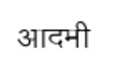
\includegraphics[scale=.6]{fig2.eps}}' (Adimx) keVLisutetx. idelAlx heVgeMdare, avanavana aBAyxsa, pUvaRgarxha, saMsAkxra ivugaLiMda hiVgAgutetxyeMdu tiLiyabeVku.

\noindent
{\bf\large{saMsAkxra visheVSavidAdxga sAhitayxda vAsatxvika pariNAma}}\label{page213}

sAhitayxvAvudeV AdarU tananxdeV Ada pariNAmavoMdanunx biVrabeVkAdare adadakekxV beVkAda kelavu ahaRteya meVle niMtideyeMdu heVLidaMtAyitu. A ahaRteyAdaru yAvudu? eMdare, saMsAkxra visheVSa. idu sAhitayxkekx mAtarxveV alalx, elAlx pariNAmakUkx anavxyisuvaMthadu. suDuvudu- uSaNxsapxshaRvu deVhadalilx PiVlAgabeVkAdare, jiVvavidAdxga mAtarx. AdadxriMda `aginxyu suDutetx' eMbudu badukiruvavanige mAtarx.

upaniSatutxgaLalilxruva `tatatxvXmasi' modalAda mahAvAkayxgaLu elAlx pApagaLanUnx suTuTxbiDutatxve- eMdare, elalxrigU anavxyavAguva mAtalalx adu. aMtaha saMsAkxrige mAtarx. adakekx beVkAda saMsAkxravu bAlayxdalelxV bidudx adariMda susaMsakxqtanAgidadxre upayoVgapaDutetx.

\noindent
{\bf\large{bAlayxda aBAyxsakekx hiridAda sAthxnavide}}\label{page213}

oLeLxyadoV keTaTxdoV! yAva saMsAkxraveV aBAyxsaveV Agali, bAlayxdalilx meYgUDidadxre kAlabaMdAga adara Palavanunx koDutetx. bAlayxdalilx bidadx saMsAkxravanunx koMcadalilx aLisalAguvudilalx. doDaDx vAyxkaraNa paMDitarobabxridadxru. avaru dashAvatAra sotxVtarxvanunx heVLuvAga avara 70neV vayasisxnalUlx saha `saMtata kaSxya imAM' eMdeV heVLutitxdadxru. alilxruvudu `saMtatakaSx ya imAM\label{213} tirxH sapatxkaqtavxH kiSxtiM' eMdu. (yAvanu ipapxtotxMdu bAri BUmiyanenxlAlxkarxtirxya rahitavAguvaMte CeVdane mADidanoV! eMdu adara athaR). Eke heVLidudx? aBAyxsakekx aSuTx hiridAda sAthxnavide eMdu tiLisuvudakAkxgi.

\noindent
{\bf\large{parxshonxVtatxragaLiMdaleV kArayx pUNaRvAguvudilalx}}\label{page213}

I riVti nAnu viSayavanunx heVLutitxruvudu nimamx manakekx taTuTxtitxdeyeVnapapx? nimamx parxshenxyanenxV namamxlilxTiTxrabahudu. athavA beVreyavara parxshenxyeV Agabahudu. utatxra koTaTx mAtarxkekx kelasa pUNaRvAyiteMdeVnU nAvu BAvisuvudilalx. EkeMdare- hasivu eMdu keVLidavanige, tiMDigaLa bage bageya sAhitayxvanonxV poVToVgaLanonxV koTaTx mAtarxkekx, hasivu nivAraNeyAgutetxMdu aMdu koLaLxlAguvudilalx. AhAravanunx nijavAgiyeV avanige koTuTx adanAnxsAvxdisuvaMteyAdAga mAtarx hasivige utatxravAguvudu `hasivu' eMdu keVLikoMDaMtahavanu AhArada pakakxdalelxV idAdxga, tegedu keYge koTuTxbiDabahudu. eSoTxV dUradalilxdudx avanu hasiveMdAga AhAraviruva jAgadavaregu avananunx karedoyudx alilx koDabeVkAguvudu. ananxda hasivuLaLx ananxgatapArxNanAda jiVviyu aSuTxdUra hoVgibiDuvudeV? ayoyxV! eMdare, hwdu KaMDitavAgiyU dUra hoVgabAradAgitutx. dUra hoVgi biTATxgideyalAlx! IgeVnumADuvudu? beVredAriyilalx. ananxviruva jAgadavarevigU sanAmxgaRdalilx tALemxyiMda sahaneyiMda naDeyutAtx sAgi ananxsikikxda kUDaleV ananxvanunxMDu savidu taqpitxhoMdabeVku.

\noindent
{\bf\large{I vicAragaLu guriyanunx lakaSxyXvAgiTuTxkoMDu sAguva sAdhakana dhaqtigAgi}}\label{page218}

Iga mADutitxruva kelasaveMthadu? eMdare- aMtaha sahanege beVkAda vasutxnishacxyavanUnx, naDedu sAgutitxruva hAdi `sanAmxgaRveV hwdu' eMba nishacxyavanUnx nimamxlilx tuMbi, niVvu aSuTxdUrada dAriyanunx naMbikeyiMda naDedu dAgalu beVkAda dADhaRyxkAkxgi koDutitxruva veYjAcnxnika utatxravAgide idelAlx eMdu tiLiriVpApx! EnoV, avana dayeyiMda ililxyavaregU baMdubiTiTxdidxVripApx!. yArU keVLali! biDali! nimagAgi koTaTx viSayagaLanunx tegedukoMDu adanenxlAlx nimamxdAgi modalige mADikoLiLxVpapx! avaneV idelalxkUkx sUtarxdhAranAgidAdxne. hiMdumuMdu noVDadeV dhaqtiyiMda iTaTx hejejx hiMdakikxDadeV vishAvxsadiMda muMde muMde sAgi! uLidudedxlalxvanUnx avanu noVDikoLuLxtAtxne. kaqSANx!

\begin{center}
****
\end{center}

\begin{center}
-\includegraphics{om.eps}-
\end{center}

(meYsUru shirxVmanamxhArAjaru koTiTxruva eraDane pArxjekfTxna utatxrakAkxgi naDesida parxvacanada sArAMsha-saMgArxhakaru shirxV enf. esf. vi matutx shirxV ke. esf. vi.)

(eraDaneya pArxjekiTxnalilx koTiTxruva padagaLu- `1. rasa, 2. dhavxni, 3. ramaNiVya, 4. alaMkAra, 5. camatAkxra, 6. shabadx, 7. vaqtitx, 9. riVti, 9. nATaka, 10. kAvayx, 11. suMdaramf, 12. shivamf, 13. sanAtanamf, 14. shAMtamf' - ivugaLige veVda, upaniSatutx, purANa, itihAsa, kAvayx itAyxdigaLa rePerenfsxnoDane vivaraNeyanunx keVLidAdxre.)

\noindent
{\bf\large{pada-padAthaRgaLa niNaRyakekx orijinalAlxda shoVdhane mADabeVku}}\label{page215}

loVkadalilx yAvudeV padada athaR, BAva, tAtapxyaR ivugaLa peYki yAvudanenxV visatxrisi tiLidukoLaLxbeVkAdare, AyA padavu yAva yAva PilfDxnalilx yAva bageya deVshakAlagaLige oLapaTuTx heVge heVge vayxvaharisalapxDutitxde eMbudanunx mwlikavAgi athaRmADikoLaLxbeVku. naMtara icACxnusAra visatxrisikoLaLxbahudu. yAvudeV vayxvahAravanunx naMbabeVkAdarU, sari-tapupxgaLa bagegx oMdu timARnakekx baMdu daqDhapaDisikoLaLxbeVkAdarU, Orijinalf Agi A bagegx saMshoVdhane mADi, muMdina hejejx iDabeVkAguvudu.

\noindent
{\bf\large{iMdu eSoTxV viSayagaLa satAyxsatayxteya niluvu mejAriTiyananxvalaMbiside}}\label{page215}

Iga eSoTxV vayxvahAragaLu heVge heVge heVgoV beLeyutatxve. adanunx `idaM itathxmf' eMdu daqDhapaDisikoLaLxbeVkAdarU janaru yAva AdhAravananxvalaMbisutAtxreMdare, adu bahujana parxyoVgaveMba mejAriTiyeMdeV Agirutatxde. suLaLxnenxV ADidarU, aMteyeV vayxvaharisidarU, adakekx mejAriTi sikikx biTaTxre adanunx satayxveMdeV naMbi, janaru nilulxtAtxreyeV horatu alilx suLuLx athavA moVsakekx eSuTx avakAshaviralu sAdhayx? eMbudanunx gamanisuva yatanxvanenxV mADuvudilalx. aSuTx dADhayxRkekx baralu kAraNaveVnu? eMdare, guMpugArikeyu nija. idu loVka vayxvahAradalilx.

\noindent
{\bf\large{shAsatxrX paraMpareyalUlx iMdu pada-padAthaRgaLa mUlavanunx shoVdhisi tiLiyuva karxmavilalx}}\label{page216}

inunx shAsatxrXda kaDe gamanisidare, yAvudAdaroMdu apUvaR parxyoVgavu pANiniya vAyxkaraNakekx virudadhxvAgi kaMDAga, yAvudeV sUtarxdiMdalU A parxyoVgavanunx samathiRsalAgadidAdxga, nAlAkxru garxMthagaLanunx magaci hAki, konege `mahAkavi parxyukatxtAvxtf sAdhu'\label{216} eMdu tiVmARnisutAtxre. hAgAdare A shabadxvu yAvudeV oMdathaRvanunx heVge koDutetx? eMba parxshenx baMdAga-

\begin{shloka}
`QuSiVNAM punarAdAyxnAM vAcamathoVRnudhAvati' ||\label{216}
\end{shloka}

eMba samAdhAna mADikoLuLxtAtxre. shabadxparxyoVga mADuvavaru `suLuLx heVLuvudeV ilalx. tapupx heVLuvudeV ilalx' eMdu samathiRsi, avarige tAveVnoV doDaDx gwrava taMdukoTaTxMte BAvisutAtxre. avarige gwrava toVrida mAtarxdiMda namageVnu lABavAyitu? adu nijaveV? suLeLxV? eMdu yathAbudidhx parishiVlisi, adariMda oMdu parxyoVjana paDeyabeVkeMba yoVcane paMDitarenisikoMDa janarige iruvudilalx. viSayavu huTuTxvAgalU, beLeyuvAgalU pArxmANikateyanunx kaLedukoMDilalxveV? adanunx naMbi, nAvu udAdhxravAgutitxdedxVveyoV? keDutitxdedxVveyoV? eMba parxshenxgU avaru jAga koDuvudilalx. vicArakekxDeyilalxdeV naMbi, naMbiyeV Ayususx mugisuvdu. hiVgAgadeV yAvudeV viSayada bagegxyU, adu huTiTxkoMDa bageyanunx parishiVlisi, adara satayxteyanunx gamanisi, Avashayxkate odagidAga adanunx naMbi, tAnu udAdhxravAgabeVku.

\noindent
{\bf\large{parxyoVgisidavara manasisxna maTaTxkekxVri padada athaRvanunx paDeyabeVku}}\label{page216}

yAvudeV padavanAnxgaliV sAhitayxvanAnxgaliV noVDuvAga parxyoVgisidavara manasisxna maTaTxkekx namamxnunx taMdukoMDu, athaRmADikoMDare adu beleyuLaLx mAtugetetx. udAharaNege- aMgaDiyalilx oMdu penf vAyxpAra mADutAtxne. adaralilx `anfberxVkabalf' eMdu hAkirutetx. adakekx `oDeyadeV iruva vasutx' eMdu nAvu athaRmADikoLaLxbahudAdarU, sutitxgeyiMda jajijxdarU, capapxDikalalxnunx meVle hAkidarU oDeyadiruva vasutx eMdu athaRmADikoLaLxbahudeV? adu nijavAgutatxdeyeV? hAgAdare A mAtige Enu aBipArxya? sAmAnayxvAgi yArobabxrU penanxnunx sutitxgeyiMda hoDeyuvudilalx. capapxDikalalxnUnx hAkuvudilalx. inunx oDeyuva parxsaMgaveMdarare keY tapipx keLage bidAdxga. aSuTx mAtarxkekx oDeyadiruva vasutx enunxvudeV `anf berxVkabalf' eMbudara athaR. `gAjinaMte puDiyAguvudilalx' eMbudaralilx tAtapxrayx. oMdu veVLe vimaNiyaMtaha gAjina padAthaRda meVleyeV `anfberxVkabalf' eMdu hAkidadxre, adanunx heVge athaRmADikoLaLxbeVku? aMdare- elAlx gAjugaLaMte alalxde oLagaDe veYranonxV matAtxvudanonxV joVDisi, tayArisiruve vasutx, `sAdhAraNagAjinaMte oDeyuvudilalx' eMdaSeTxV athaR. adara meVle guMDukalulx hAkidarU oDeyuvulalx? eMdu pariVkiSxsa horaDabAradu. I bagegx nAleDfjx barabeVkAdare, `yAva pada sAhitAyxdigaLu yAva TeYM-sepxVsinalilx upayoVgisalapxTiTxve' eMba aMshavanunx parishiVlisi, athaRmADikoLuLxva aBAyxsa beLeyabeVku.

\noindent
{\bf\large{vividhavAda athaRgaLalilx rasapadavu baLakege baMdide}}\label{page217}

\begin{itemize}
\item[(1)] Iga `rasa' viSayavanunx noVDoVNa-\\
I padavanunx yAvA yAvA saninxveVshadalilx heVge heVge upayoVgisutAtxre? noVDi!.
\item[(1)] `avanu bahaLa rasavatAtxgi mAtADida' enunxtAtxre. daqSATxMtoVdAharaNegaLoMdige manasisxge hiDiyuvaMte mAtADida eMdathaR alilxya `rasa' shabadxkekx.
\item[(2)] `avanoDane mAtanADuvudaralilx rasavilalx' enunxveDeyalilx, upayoVgavilalx, AdabeVkAda viSayakekx avana kaDeyiMda poVSaNeyilalx, avanu adanunx AdaravAgi tegedukoLaLxlAra, eMdathaR barutetx.'
\item[(3)] `avanu sarasavAgi mAtanADutitxdadx' eMdAga, nagu nagutAtx tamASeyAgi mAtADutitxdadx eMba aBipArxya barutetx.'
\item[(4)] `avanu oLeLxya rasavAgidAdxne. avananunx karedukoMDu baninx. namamx kelasa Agutetx' aMdAga tAkatAtxgidAdxne- balashAliyAgidAdxne eMba Ashaya
\item[(5)] `avanu oLeLxya rasika. AdadxriMda avanalilx mAtanAnxDabahudu' aMdare, mUlABipArxyadoDane mAtananxthaRmADikoLuLxtAtxne. namamx mAteVnU veYpariVtayxkekx tiruguvudilalx. keVLidudx sAthaRkavAgutetx eMdathaRbarutetx.
\item[(6)] adeV rasaveMba padaveVnAdarU veYdayxra kivige bidadxre, `mUlikeyanunx hiMDida darxva' eMdAgutetx.
\item[(7)] `rasa'veMba padavanunx sidadhxveYdayxrArAdarU keVLisikoMDare pAdarasa-pArada eMdukoLuLxtAtxre.
\item[(8)] `oLeLxya rasavAda pAka' eMdare- madhurAdi SaDarxsAnxna eMbathaRdalilx nilulxtetx.
\item[(9)] kavigaLu, sAhitayxkAraru ivarugaLu I padavanunx heVLuvAda shaqMgArAdi navarasagaLu eMdathaRkoDutetx.
\item[(10)] veVdAMtigaLu rasa pada keVLidare, `rasoV veY saH'\label{223} eMdu heVLalapxDuva paramAtamxneV adara athaR eMdu tegedukoLuLxtAtxre.
\item[(11)] iMdina vidAvxMsaru `oLeLxya rasika' eMdeVnAdarU heVLidare, yAvudeV mAtanUnx kAmukajiVvanada athaRdalilx tegedukoLuLxtAtxne - eMdathaR.
\item[(12)] I pada keVLidAga cikakxMdina rasaveV beVre, iMdina rasaveV beVre, inUnx kelavu kAla kaLedare aMdina rasaveV beVre- aMdAga `rasa' eMdare pakavxte eMdathaRbarutetx
\item[(13)] `samarasavAda jiVvana matutx vayxvahAra' eMdAga BinAnxBipArxyavilalx viroVdhavilalx' eMdathaR. iSeTxV alalxveV inUnx vividhavAda athaRdalilx `rasa' padavu vayxvahArakekx baMdide. I bagegx koVshavanunx noVDuvudAdare- shaqMgArAdiSu navasu, lavaNAdiSu SaTusx, pAradeV, rAgeV nirAyxsa viVrayxguNa dhAtu viSaGaqtAdw ca rasaH porxVkatxH eMdide.
\end{itemize}

\noindent
{\bf\large{parxshinxsidavara Ashayavanunx gurutisi vivaraNe koDabeVku.}}\label{page218}

hiVge padakekx aneVkAthaRgaLidAdxga, `rasa' padada hiMde `shaqMgArAdi', `madhurAdi' itAyxdiyAgi visheVSaNavAvudU ilalxdidAdxga keVLuvavanu `rasa' padakekxVnu athaR? eMdu parxshenx mADidare, utatxrakoDuvavanu nimamx parxshenx yAva parxkaraNadalilxruva `rasa' padada bagegx? eMdu maru parxshenx hAkabeVkAgutetx. `rasa' padakekx eSuTx athaRgaLiveyoV adanenxlAlx heVLibiDi- aMdare, niGaMTuvanunx tegedu, elAlx athaRgaLanUnx heVLibiTuTx iSuTx athaRgaLive enanxbeVku. naMtara ivugaLalilx nimage yAvudu beVkoV adanunx selekfTx mADikoLiLx enanxbeVkAguvudu. yAvudAdaroMdu guMpinalilxratakakx padavAdare, A guMpu yAva parxpaMcakekx seVridodxV adanunx noVDi heVLabeVkAguvudu, Iga avaru koTaTx padagaLelAlx kAvayx parxpaMcakekx saMbaMdhapaTaTxdAdxgi kaMDu baMdiruvudariMda, adu veYdayxkAkxgaliV UTakAkxgaliV saMbaMdhisidadxlalxveMdu nishacxyisi muMdina mAtanAnxDabeVkAguvudu.

\noindent
{\bf\large{utatxrisuvAga parxshinxsuvavana manaHpakavxteyanUnx gamanisabeVku}}\label{page219}

iSeTxlAlx vicAradiMda I padavu kAvayx parxpaMcada siVmeyalilxruvudeMdu tiLidarU, adu shaqMgArAdiyeV eMdu gotAtxdarU, parxshenx mADidavana pakavxte (nAleDfjx) yanUnx ililx gamanisabeVkAguvudu. rasada viSayavananxthaRmADikoLaLxlu beVkAda rasikate avanalilxdeyeV? eMbudanUnx nishacxyisikoLaLxbeVku. EkeMdare- ideV pada makakxLa kivige bidudx, avarugaLu `kAvayxgaLalilx baLasuva rasada vicAravAgi nanage tiLisi' eMdu keVLikoMDAga, `huDuga budidhxvaMta rasada viSayadalilx keVLibiTaTx' eMdu higigxkoMDu rasagaMgAdhara- sAhitayx dapaRNa- kAvayxparxkAsha- BaratananATayxshAsatxrX elalxdariMdalU viSaya tegedu AyA koTeVshanfgaLoDane vivaraNe koTuTx `rasa hiVgide - noVDapApx!' eMdare. parxshenx avaniMda baMdudu nijavAdarU, utatxra avanige eSuTx upayoVgavAdiVteyeMdU nAvu parishiVlisabeVkAguvudu. idakekxVnu kAraNa? eMdare heVLuva viSayavanunx manasusx garxhisalu oMdu vayasUsx, matutx avaralilx beLavaNige hoMdiruva parxvaqtitxgaLU beVkAguvudu.

\noindent
{\bf\large{viSaya garxhaNadalilx avanavana kaMDiVSanfgU oMdu hiridAda pAtarxvide}}\label{page219}

aMteyeV I kAraNagaLa jotege avanavana kaMDiVSaninxgU hiridAda pAtarxvideyeMbudanunx mareyabAradu. EkeMdare- javxra piVDitanAdavanalilxge hoVgi, `oLeLxya aMboDe mADede, tinunxtitxVyA?' eMdu keVLidadxre heVgoV hAgeyeV muKavikAraveVpaRDutetx. `hAlu KiVru kuDiyutitxVyA?' eMdare, `A hALu kiVru hatitxra taraleV beVDa' eMdu heVLabahudu. avanu AMboDeyanunx oMdu kAladalilx capapxrisikoMDu tiMdiralilalxveV? hAluKiVru tegedukoMDu inUnx savxlapx hAki eMdu kuDidiralilalxveV? adara viSayaveV gotitxlalxdavaneVnalalx. hAgAdarU Eke hiVgAgutetx? eMdare, avanige baMdiruva javxrada kaMDiVSanf I taraha mADisutetx. I riVti catuviRdhavAda ananxvU KAdayx coVSayx leVhayx peVya' elalxvU muKa vikAsakekx badalu muKa vikAravanenxV odagisutetx. A padAthaR A pada elalxvU asahayx sUcisuva muKakekxV kAraNavAgutetx. EneV parxyatanxmADidarU rasavatAtxda vasutxvina bagegx rasoVdobxVdhavAguvudilalx. savxlapx savxlapxvAgi nAlageyalilx ruciyuMTAgalu shuruvAdare, `A vasutx ideyeV? I vasutx ideyeV? idanunx tiMdare bAdhakaveV?, I riVtiyAgi oMdoMdAgi shuru mADutAtxne. idakekxlAlx Enu kAraNa? eMdare pitatxvu rasagarxhaNa mADuva AyA keVMdarxgaLanunx mucicxdAdxga hAganinxsutitxtutx. pitatxvu jAga biTuTxkoDalu AraMBavAda meVle DAkaTxraru heVLida pathayxveV beVjArutarutetx. modalu rasadalUlx kasakAnuTiTxdadx nAlage, kaMDiVSanf badalAyisutAtx kasadalUlx rasa kANalu pArxraMBisitu enanxbeVkAgutatxdeyalalxveV? hiVge deVhada viSayada bagegx ruci arucigaLige kAlavU kAraNavAgirutatxde. kaMDiVSanf meVle mAtarxveV rasa virasagaLalalx. caLigAla maLegAla beVsige kAla ivugaLa meVlU, upupx huLi KAra modalAda rasagaLalilx ruci arucigaLa veYpariVtayx huTuTxtetx. caLigAladalilx KAra upupx rasagaLu hecAcxgi hiDisutetx. AvAga adara vaNaRnegaLanunx keVLidareVneVV bAyalilx niVrUralu shuruvAgutetx. I samayadalelxVnAdarU niMbeVhuLiyu pAnakavanunx koDuvudAgaliV, vaNiRsavu dAgaliV mADidare, rucisuvudilalx. adu yArige beVku daridarx enunxtAtx, adeV bisilu kAla baMtu eMdare, pAnakaveMda kUDaleV amaqtadaMte adakekx hAtoreyuvaMtAgutetx. adara hesareV amqta. adanunx taMdu koTaTxvaranunx A pAnakakikxMta taNaNxgiruva noVTadiMda noVDi, `shataM jiVva eMdAshiRvARda mADuvaMtAgutetx. hiVge ruci- arucigaLige kAlavU kAraNavAgutetx. I daqSiTxyiMdaleV kAla-deVsha-kaMDiVSanunxgaLanunx parishiVlisiyeV yAva viSayada vivaraNeyanAnxdarU koDabeVku eMdu heVLidudx.

\noindent
{\bf\large{dAMpatayx jiVvanavidadxvarigelAlx `shaqMgAra rasa'da paricayaviruvudilalx -}}\label{page221}

shaqMgArAdi rasada bagegx nimageV vivaraNe koDabeVkAdarU adakUkx oMdu saninxveVshabeVkAguvudu. nAnu hAgaMdAga nimage AshacxyaRvAgabahudu. ideVnu? namage heMDati makakxLilalxveV? namage shaqMgArarasa gotAtxguvudilalxveV? eMdu. Adare heMDati-makakxLu idadx mAtarxdiMdaleV shaqMgArarasavu athaRvAgididxrabeVkeMba niyamavilalx. heVgoV pashupakiSx sAdhAraNavAda matutx vayaHparxyukatxvAda deVha dhamaRdiMda (kAmadiMda) dAMpatayx jiVvana naDedideyeV horatu AyA rasagaLu baMda karxmadoDane AyA rasagaLanunx tegedukoMDu kelasaveVnU naDedilalx.

\noindent
{\bf\large{AhAra seVvaneyalUlx rasagaLanunx saviyadiruvuduMTu}}\label{page221}

shaqMgArAdi rasagaLu mAtarxvalalx, BwtikavAda SaDarxsagaLa vicAradalUlx hiVgeyeV rasagaLananxriyadeyeV UTa tiMDigaLu naDeyabahudu. heVgeMdare bahaLa hasivAgidAdxga athavA APiVsf, PAyxkaTxrigaLige horaDuva tavxre idAdxga puLiyoVgare, sakakxre poMgalu, dadhoyxVdana idAvudanenxV baDisidarU nAma, rUpa, rasagaLa viBAgaveV ilalxde bAyige hAkikoMDu, gaMTalige taLiLx, nuMgi, UTada kelasa mugisabahudu. AdadxriMdaleV `kuSxdhAturANAM na rucinaRpakavxmf'\label{221} eMdu heVLutAtxre. A samayadalilx avanige beVkAdudx hasivaninxMgisuvudu mAtarxveV, rasagarxhaNavalalx. avanalilx hoVgi puLiyoVgarege upupx heVgitutx? eMdu keVLidare `OhoV! nAnu adanunx gamanisaleV ilalx. inonxmemx hAki, noVDi heVLutetxVne' enunxtAtxne. naMtara huLi heVgitutx? eMdare `Iga upapxnunx mAtarx gamaniside. huLiyanunx gamanisaleV ilalx. inonxmemx hAki' enunxtAtxne. hiVge yAva rasada bagegx avaru parxshinxsidaroV, adakekx mAtarx utatxra koDutAtxne. oMdoMdu rasakAkxgiyU, oMdoMdu sala hAkisi koLaLxbeVkAgutetx. I taraha alalxde, omemx bAyige hAkikoLuLxvAgaleV elAlx rasagaLanunx paqthakf, paqthakAkxgi garxhisiyU avugaLalilx sAmarasayxvanunx gamanisikoMDu UTa mADutitxrabeVkAdare adakekxV beVkAda oMdu parxvaqtitxyU, shakitxyU beVkAgutatxde.

\noindent
{\bf\large{rasa keVMdarxgaLU paTuvAgidudx, garxhisuva parxvaqtitxyU idadxre rasavanunx garxhisalu sAdhayx}}\label{page222}

parxtiyoMdu rasakUkx nAligeyalilx beVre beVre keVMdarxgaLive. AyA keVMdarxgaLu paTuvAgi avugaLanunx garxhisuva parxvaqtitxyU idAdxga, AyA rasagaLa arivu dorakutatxde. rasagarxhaNa keVMdarxgaLalilx balavu kaDimeyAdAga, matutx garxhisuva parxvaqtitxyu ilalxdAdaga, yAva rasavU arivAguvudilalx. hAgeyeV navarasagaLalilxyU saha AyA keVMdarxgaLige paTutavx, parxvaqtitx ivugaLidudx budidhxsUkaSxmXte, rasikate ilalxdidadxre avasaradalilx tiMdAga kuSxninxvAraNe AguvaMte ililxyU kAmanivAraNe, kAma shAMti AgabahudaSeTxV horatu rasajacnxtege avakAshavilalx. idanenxV `kAmAtureV noV rasaBiVtilajAjxH'\label{222} enunxtAtxre. obabxnige BagavatapxrXsAdavAda hAluKiVru cenAnxgirabahudu. matotxbabxnige bisiniVru mAtarxveV cenAnxgirabahudu. adelAlx AyA saninxveVshada Avashayxkateya meVle nilulxtetx. alelxlAlx rasABivayxkitxge viSayaviruvudilalx. AdadxriMdaleV shaqMgArAdi rasagaLanunx vivarisabeVkAdarU alolxMdu saninxveVsha beVkeMdu heVLidudx.

\noindent
{\bf\large{navarasagaLu SaqSiTxsahajavAgive}}\label{page222}

I rasaveMba padAthaRvu saqSiTxsahajaveV? athavA kaqtirxmaveV? eMdu parishiVlisidAga saqSiTx sahajaveMbudeV sariyAda utatxra. obabx ceVtananu huTuTxvAgaleV avana huTiTxnoMdige I rasaveMbudU seVrikoMDeV iruvudu. koVpaveMbudu yAva isivxyalilx huTiTxtu eMdare adakekx yAva isivxyU ilalx. parxkaqtiyalilx huTuTxva parxkoVpakekx yAva isivx heVLoVNa? adaraMte namamxlilx huTuTxva koVpakUkx isivx heVLalAguvudilalx. kAmakUkx hAgeyeV. ivugaLaMteyeV shaqMgArAdi navarasagaLU saqSiTx sahajaveV Agirutatxve. BagavaMtanigU I shaqMgAravuMTapApx. Adare namamxMte kuSxlalxka shaqMgAravalalx. udAtatx shaqMgAra. A udAtatxshaqMgAravU savxBAvavAgiyeV avana rasavAgide. adanenxV `shaqMgAraM kiSxtinaMdanAviharaNeV' eMdu heVLuvudu.

\noindent
{\bf\large{`rasa'vu paramAtamx savxrUpaveV Agide}}\label{page222}

mUlaButavAgi yAva oMdu rasavideyoV adanenxV veVdavANiyu-

\begin{shloka}
`rasoV veY saH | rasaM heyxVvAyaM labAdhxvX AnaMdiV bavati' |
\end{shloka}

eMdu sArutitxruvudu. rasavu paramAthaRdalilx nilalxbeVkAdare alilx tAneV. adu paramAtamx savxrUpaveV. adu darxviVButavAgi muMduvaridAga alilx tAneV shaqMgArAdi rasagaLu. adu GaniVBUtavAgi niMtu biTaTxre muMdakekx loVkadalilx yAva rasavU ilalx.

\noindent
{\bf\large{SaDarxsa hAgu navarasagaLu}}\label{page223}

madhurAdi SaDarxsagaLu jiVviya nAligege viSayavAguvudAradare, shaqMgArAdi navarasagaLu avana manasusx matutx budidhxgaLige viSayavAgutatxve. AyA rasagaLanunx ebibxsi aMdare udoBxVdhagoLisi, manoVbudidhxgaLige viSayagoLisuva sAmagirxgaLu mAtarx beVre beVre eSoTxV vidhavirabahudu. aMtha sAmagirxgaLa peYki suMdaravAda kAvayxvU oMdAgide. 

\noindent
{\bf\large{`vayxvahAra' padAthaR vivaraNe}}\label{page223}

Iga I rasavanunx kAvayxdalilx yAva riVti tegedukoMDidAdxre? eMba viSayadalilx kelavu mAtanAnxDabeVkAgide. A daqSiTxyiMda rasaveMdareVnu? BAvaveMdareVnu? kAvayxparxpaMcakekx saMbaMdhapaTaTxMte I rasaBAvagaLa vayxvahAravanunx vicAraBUmiyalilx heVge taMdidAdxre? alalxde anAdikAladiMdalU aMdare saqSiTxyu AraMBadiMdalU vayxvahAraveMbudoMdu barutitxdeyalalx A vayxvahAravu I rasa-BAvagaLa viSayadalilx heVge barutitxde? adu yAva vayxvahAra? iSuTx parxshenx hAkikoMDu, ivugaLigelAlx utatxrisuva munanx sAvaRtirxkavAgi vayxvahAraveMdareVnu? eMbudanunx parishiVlisoVNa.

vayxvahAra enunxvAga vi+ ava+ hAra iSuTx aMshagaLive. ililx madheyx iruva `ava' eMba upasagaRvu `apa' eMba upasagaRda samAnAthaRvAgide. udAharaNege - AvakaSaR, apakaSaR iveraDU samAnAthaRka. aMteyeV avamAna apamAna- iveraDU samAnAthaRka.

\begin{shloka}
`parxtikatuRM parxkaqSaTxsayx nA\char'263vakaqSeTxVna yujayxteV |' (rAmAyaNa)\\\label{223}
`paNoV deVyoV\char'263vakaqSaTxsayx SaDutakxqSaTxsayx veVtanaM' | (manusamxqti 7.1.126)\label{223}
\end{shloka}

ililx `utakxqSaTx' eMba padakekx eduru padavAgi baLasiruva `avakaqSaTx' padavu apakaqSATxthaRdalilxde eMbudanunx gamanisabahudu. aMteyeV avahAra padavu apahArAthaRkavAgide.

aMteyeV yAsakxnirukatxdalilx-

\begin{shloka}
`aBaRkaM kasAmxtf? avahaqtaM Bavati' (avahaqtaM - apahaqtamf)\\\label{224}
sidAdhxMta kwmudiyalilx - `kuDavamavaharati' (avaharati - apaharati)\\
mahABAratadalilx- `EvaM rAjananxvahAroV baBUva'\\\label{224}
`tatoV\char'263vahAraM seYnAyxnAM tava teVSAM ca BArata!'
\end{shloka}

I parxyoVgagaLalelxlalx `ava' eMbudu `apa' eMbudara athaRdalilxdeyeMbudanunx gamanisabahudu. iMtaha avahAravanunx - apahAravanunx vAyxvaqtitx mADuva kirxyeyeV vayxvahAra. (vigataH avahAraH yatarx saH vayxvahAraH) parxtiyoMdu vasutxvU, saqSiTx koTaTx guTukAgi baMda tananxtanavanunx athavA tananx dhamaRvanunx beLesi uLisikoMDu hoVgutitxruvAga, adanunx apaharisi adara hakukx kaLeyalu yAvudAdarU baMdare, adanunx parxtiBaTisi, apahArakekx virudadhxvAgi hoVrADuvudu. aMtaha kirxyeyeV vayxvahAravenisuvudu. I vayxvahAravu, saqSaTxvAguva elAlx vasutxgaLalilxyU sahajavAgide. tananx tanavanunxLisikoLuLxva kirxyeyeV vayxvahAra. idu saqSiTxya AraMBadiMdalU, elelxlUlx eMdeMdU iruvudAgide. mwlikavAgi ideV vayxvahAravAgidudx, I aMsha mAtina mUlaka baMdare adU vayxvahAraveV. I vayxvahArakekx mwlika vayxvahAradoDane savxlapxvU BinanxteyilalxdeV idAdxga pArxmANika vayxvahAra, Binanxte kaMDu baMdAga moVsada vayxvahAra, kapaTa vayxvahAra eMba shabadxgaLu huTiTxkoLuLxtatxve. pArxmANikaralilx parishudadhx vayxvahAravU, aparxmANikaralilx moVsa-kapaTagaLa vayxvahAravU huTiTxkoLuLxtatxve. iSuTx vayxvahAraveMdareVnu? eMbudanunx tiLisuva saluvAgi. loVkadalilx vayxvahAraveMba hesariniMda baMdiruva vayxvahAravelAlx shudadhxvAgideyenanxlAguvudilalx.

\noindent
{\bf\large{rasaBAvagaLa viveVka}}\label{page224}

tiLisida iSaTxMshagaLanunx manasisxnalilxTuTxkoMDu, rasa-BAvagaLa viSayadalilx anAdi vayxvahAra heVge beLedu baMtu? naMtara kAvayx parxpaMcakekx baMdAga, I rasa BAvagaLa vayxvahAravu heVge beLeyitu? eMbudanunx parishiVlisabeVkAgide.

`bAhAyxthaRvanAnxsharxyisi huTuTxva manasisxna oMdu vikAraveV BAva'

`A BAvada utakxSaRveV rasa.'

eMdu rasa BAvagaLanunx vivarisutAtxre. I bagegx saMsakxqta vAkayxvidu-

\begin{shloka}
`bAhAyxthARlaMbanoV yasutx vikAroV mAnasoV BaveVtf |\\\label{225}
sa BAvaH kathayxteV sadiBxH, tasoyxVtakxSoRV rasaH samxqtaH ||' eMdu.
\end{shloka}

(rasa-BAvagaLa bagegx viveVcane noVDi) oMdu dArxkiSxya haNuNx bahaLa ruciyAgideyaSeTxV. adu asAvxdaniVyavAgiruva kAraNa adanunx rasayxvAgide enunxtAtxralalxveV? Adare adu haNANxguva munanx miDiya desheyalilx tiMdu noVDidare, A rasaviruvudilalx. oMdeV vasutxvinalilx atayxMta rasavatAtxgiruvudU, rasahiVnateyU eraDU heVge sAdhayx? eMdare, yAvudeV vasutxvinalUlx rasayxte baruvudu oLeLxya vikAsadiMdaleV AdadxriMda, miDiyalilx vikAsaveVpaRDada kAraNa rasavu inUnx baMdilalx. muMde AgabeVkAgide. vikAsAvasethxyalelxV rasapUtiRyAguvudu. pUNaRrasadalelxV AsAvxdayxte baruvudu. I daqSiTxyiMda gamanisidAga rasa matutx BAvagaLa sAthxnamAnagaLananxLedukoLaLxbahudu. `BAva'veMbudu, oMdu miDiya sAthxnadalilxdadxre; `rasa'veMbudu, paripakavxvAda Palada sAthxnadalilxruvudAgide. moda modala avasethxyalilx adu BAvavenisikoLuLxtetx. naMtara vikAsavAdaMtelAlx adaralilx rasatavxveVpaRDuvudu. BAvaveMbudeV beLedu vaqdidhxhoMdi mAgidAga rasavAgutetx. sariyAgi heVLidare, BAvavikAsaveV rasa. Adare ivarugaLu EnanunxtAtxreMdare? inAnxvudoV oMdara vikAraveV BAvaveMdu. nijavanenxV noVDi heVLuvudAdare, vikArarahitavAda sithxtiyeV BAva. (AdadxriMda `sAthxyiVBAvaH' enunxvudu. vikAravAguvudAdare adu heVge sAthxyiyAdiVtu?)

\noindent
{\bf\large{shAsatxrXdalilx baMda `vikAra' padAthaR vivaraNe}}\label{page225}

BAvada vikAsaveV rasa. ivareVke hiVge heVLidAdxre? eMdare- adara aBipArxyavanunx hiVge tegedukoLaLxbahudu. `bAhAyxthaR'veMdare bahiriMdirxya goVcaravAgatakakx vasutxgaLu. avugaLa meVle namamx daqSiTxyanunx hariyisi noVDidAga, satatavikArAtamxkagaLAgiyeV A vasutxgaLiruvudu kaMDubarutatxde. vikArAtamxkavAda vasutxgaLa saMbaMdhadiMdAguvaMtha parxtikirxyeyanunx avikAraveMdu BAvisuvudu heVge? AdadxriMda aMtaha BAvavanunx `vikAra' eMdaru. ililx `vikAra' eMdare pariNAmaveMdathaR. adariMda manasisxnalAlxguva pariNAmavu vikAsa rUpa. manasisxna sithxti visheVSavAdadxriMda `BAva'venisalapxTiTxtu. I sithxtiyeVnU manasisxnalilx modaleV sAvaRkAlikavAgi acacxLiyadeV iralilalx. muMdU iruvudilalx. sAMkeVtikavAgi nAvu EneVnoV BASegaLanunx kaTuTxvudu beVre. neYjavAgi iruvudu beVre. vikAsavU vikAravU oMdeV AyitalAlx! aMdare- kAraNAvasethxyanunx parxkaqtiyeMdU. kArAyxvasethxyanunx vikaqti-vikAra eMdU dAshaRnikaru vayxvaharisuvaru. mogigxna kArAyxvasethxyeV hUvu. adeV vikAsa. kArAyxvasethxyAdadxriMda vikAsa rUpavAda pariNAmavanunx vikaqti-vikAra enunxvudu. vikAraveMdu hiVyALisuva athaRvalalx idu. vikAsavU oLagina dhamaRda aBivayxkitxyeV AdadxriMda, aBivayxkatxvAguvaMtaha dhamaRvu namage veVdayxvAguvudu kAladeVsha siVmegoLapaTaTxrU- aMdare aBivayxkitxyu tAtAkxlikavAdarU, A dhamaRvu shAshavxtavAdadxriMda adu niviRkAra eMbudU sariyAdudeV. `BAva' eMbudanunx heVge heVgoV sutitx baLasi vayxvahArakekx taMdide loVka. iSeTxV alalxdeV vikAravuLaLx padAthaRgaLanenxV BAvaveMdU heVLidAdxre. `SADABxva vikAragaLu'\label{226} enunxtAtxralAlx! beVre beVre avasethxgaLanenxV hoMdadeV vikAsaveMbudeV Agadu. avasAthxMtara pArxpitxyu tAneV vikAra. AdadxriMda BAva parAyxyavAgi vikAra padada vayxvahAraveVpaRTiTxde.

\begin{shloka}
SaDABxva vikArAH BavaMtiVti vASARyxyaNiha | \\
jAyateV, asitx, vipariNamateV, vadhaRteV, apakiSxVyateV, nashayxti iti ||' -eMdu.
\end{shloka}

\noindent
{\bf\large{BAvavananxnusarisi hAva, alilxMda muMde shaqMgArAdi rasagaLu}}\label{page226}

BAvavu avikAravAdadudx eMdare, AsatayxrUpavAda BAvaveV aMthAdudx. adeV ivelalxkUkx mUla. adariMdaleV parxpaMcada samasatx vayxvahAravU naDeyutitxruvudu. loVka saqSiTxyu muMduvariyalu modalige mUlavAgi puruSa matutx sitxrXV eMba eraDu vasutxvU idAdxga, puruSanalilx vayxkatxgoLuLxva Atamx BAvaveV moTaTxmodalaneya BAva, naMtara alilxMda muMdakekx A BAvavu aBivayxkitx hoMdidAga, A BAvakekx takakx hAvaveMbudoMdu sitxrXVyalilx huTiTxkoMDu, AnaMtara shaqMgArAdi rasagaLu huTiTxkoLuLxvuvu.

\noindent
{\bf\large{BAva, hAvagaLu tAMDava hAgU lAsayxgaLAguva sahajavAda naDeyanunx puruSa hAgU sitxrXVyaralilx gurutisabahudu}}\label{page226}

ililx puruSanalulxMTAda BAvadiMda, avana balaBAgada calaneya mUlaka, I riVtiya tAMDavavoMdu mUDuvudAdare, adara parxtikirxyeyAgi sitxrXVyAdavaLige eDagaDeya calaneyiMda I riVtiya lAsayxvu mUDutatxde. (tamamx deVhada niluviniMda tAMDava-lAsayxgaLa BeVdagaLanunx suPxTavAguvaMte toVrisidaru.) heMgasarige yAvAgalU vAma pAshavxRveV (eDaBAga) hecAcxgi kAyaRdalilx pAlogxLuLxtatxde. gaMDasarige balaBAga pAlogxLuLxtatxde. udAharaNe- gaMDasAdavanu heMgasanunx kuritu, `yAvotutx niVnu hiVgeyeV mADuvudu' eMdu gadarisutAtx bala BAgavanunx muMdoDiDx niMtare, heMgasAdavaLu meYyalilx koMku koMkugaLoDaneV, `hwdu, hwdu nAnu yAvotUtx hiVgeyeV' eMdu heVLutAtx tananx meY eDapAshavxRvanunx hiMdakekx bAgisi niMtu utatxrisuvaLu. idu parxkaqti sahajavAda naDe. AdadxriMdaleV avaLanunx `vAmAMgiV, vAmaloVcanA' eMdelAlx hesarisiruvaru. gaMDu biVriyenunxvavara vicAra beVre, adanunx nAnililx seVrisilalx. (adakekx kAyaRkAraNagaLu beVre) puruSanalilx BAva. sitxrXVyaralilx hAva. BAvada parxtikirxyeyeV hAva. baratAcArayxru tamamx nATayx shAsatxrXdalilx-

\begin{shloka} 
`yoV veY BAvaH sa EveYSaH shaqMgArarasasaMBavaH'\label{227}
\end{shloka}

eMdu heVLidAdxre.

\noindent
{\bf\large{shaqMgAraveV modala rasa}}\label{page227}

obabx puruSa, oMdu parxkaqti, iveraDu seVruva kaDe parxparxthamavAgi shaqMgAra. idanenxV-

\begin{shloka}
`yaH sitxrXVpuruSa (yoVyoVRgaH) saMyoVgaH ratiH saMBoVgakArakaH |\\\label{227}
sa shaqMgAra iti jecnxVyaH upacArakaqtaH shubaH |'
\end{shloka}

eMdU heVLidAdxre. yAva oMdu vasutxvu moTaTx modalige savxyaMjoyxVtiyAgi beLaguvudAgidudx, kAla visheVSadalilx tAnu vikAsavAgalu horaTu oMdu sithxti paDeyuvudoV, alilx oMdu shaqMgArarasa. adeV modala rasa. naMtara karuNAdigaLu. AdadxriMda shaqMgArAdi rasagaLeMba vayxvahAravAgide. karuNAdi rasagaLeMdArU vayxvaharisuvudilalx.

\noindent
{\bf\large{rasAnuBavavu yArige? yAvAga?}}\label{page227}

(inunx rasada neleya bagegx ciMtisoVNa) rasaveMba padAthaRviruva jAga yAvudu? nAvu yAva padAthaRvanunx saviyutetxVvoV adaralolxV? yAru saviyutAtxnoV avana haqdayadalolxV? eMdu viveVcane mADabeVku. udAharaNege- sumadhuravAda oMdu rasapUri mAvina haNaNxnunx tegedukoMDare, adeVnU tananx guNavanAnxgaliV rasavanAnxgaliV heVLikoLuLxvudilalx. alilx adanunx AsAvxdisuva riVtiyalilx tinunxvavanidadxre, avanu adanunx heVLikoLaLxbeVku. padAthaRvU idudx adanunx saviyuvaMtaha iMdirxyavU idudx averaDara saMyoVgavU EpaRTATxga alilx oMdu rasa. aMteyeV yAvudAdarU oMdu BAvavidudx adu visAtxravAgalu shuruvAdAga alilx oMdu rasakekx avakAsha. sitxrXV-puruSaru oMdAgi kaletu. saMBoVgisidAga alilx oMdu ceVtanavu tAneV `saMBoVgiside, rasAnuBavavAyitu. `nemamxdi paTeTx' eMdu heVLikoLaLxbahudu. alilx ceVtananeV ilalxdeV, keVvala horagaDe oMdu gUDidaMtaha iMdirxyAkAragaLu mAtarxveV saMBoVga mADalU, `rasavAgi suKapaTeTx' eMdu heVLikoLaLxlU avakAshavilalx. AdadxriMda ililx bAhayxvAgi rati suKavananxnuBavisidavanU ceVtananeV.

\noindent
{\bf\large{bAhayxvAda ratiyu AMtaravAda ratiyoMdige EkiVBUtavAdAga rasa}}\label{page228}

iMtaha ceVtananige bAhayxvAda ratiyu heVgoV hAgeyeV AMtaravAda AtamxratiyU uMTu. bAhayxratiyeMbudu BwtikavAdare matotxMdu AdhAyxtimxkavAdudu. A AMtaravAda Atamxratiya rasavanunx kaMDu uMDu savidu divAyxnuBava paDeda mahApuruSaru, adanunx mareyadeyeV idudxkoMDu horagaDeyU vAyxpaqtarAguvaMtAdAga alilx naDeyatakakx bAhayx ratiyU saha A AdhAyxtimxka ratiyalilx seVpaRDeyAgi EkiVBavisuvaMtAgabahudu. hAge ramisuvaMtAdare mAtarx, alilx adoMdu yajacnxvAgi pariNamisuvudu. AvAga `yajacnxkaSxpita kalamxSAH'\label{228} eMdAgalu avakAshavAguvudu. AdadxriMda ratiyU saha oMdu udAtatx sAthxnavanunx hoMdide.

\noindent
{\bf\large{shirxVmadABxgavatadalilx visAtxragoMDiruva shaqMgArada hinenxle}}

I ratiyeV shirxVmadABxgavatadalilx visAtxravAgi vivarisida rasa. A mahA puruSanAda shirxVkaqSaNxnU saha goVpasitxrXVyaroDane heVge ramisida? eMba parxshenxbaMdAga, hiVge, inAnxriMdalU ramisalAgada pavitarxtamavU jaganamxMgalavU Ada riVtiyalilx- viratiya paramAvadhiyalilx ramisida- enunxva aMshavanUnx pakakxdalelxV kANabahudAgide. avanu hiVge goVpasitxrXVyaroDane mAtarx ramisalilalx, goVpAlakaroVdige ramisidanapapx! adanenxV `goVpAnf saMBarxmayanf'\label{229} eMbudariMda tiLidukoLaLxbahudu. aMteyeV `goVgoVpagoVpiVjanamadhayxsaMsathxM'\label{229} eMbudU gamanisatakakxdudx.

hiVgAgalu beVrobabxriMda heVge sAdhayx? avanu `puMsAM moVhana rUpanU AgidAdxne- puMsAmapi moVhanarUpanivanu. jaganomxVhananivanu. avanu tanagAgiyeV iTuTxkoMDa divAyxtamxratiyapApx!

\noindent
{\bf\large{BAvaveV haridu baMdu rasavAgutatxde}}\label{page229}

idu A moTaTxmodalinadAda shaqMgArarasa. nUrAru keY dATi namamxvarege baMdu I bageya shaqMgArarasavAgide. iMtaha pariNAmakekx baMdu niMtide. I dajeRya shaqMgAravanUnx saha obabx SaMDanu heVLikoLaLxlAra. viVranAgi savxlapxvAdarU BAvukate iruvavanu mAtarx tAneV heVLikoLaLxbeVku. puruSanAda obabx ceVtananalilxruva BAvavidu. BAvavu I bageyalilx haridu baMdu rasavAgutatxde.

\noindent
{\bf\large{udAtatx vayxkitxtavxgaLalilx shaqMgArAdi rasagasaLa pUNaR AsAvxda}}

I shaqMgAra-viVrAdi rasagaLu namamxMtahavara jiVvanadalUlx uMTu. aSuTx mAtarxvalalx. pashupakAvxyXdi pArxNigaLa jiVvanadalUlx ideV rasavuMTu. elAlx rasagaLu uMTu. Adare avugaLalilx obabx kaviyu AsAvxdane mADuva tarahada AsAvxdanege eDeyilalx. mAnavaralUlx rasagaLa AsAvxdane ilalxdiruvuduMTe? eMdare asaMBavavenunxvaMtilalx. paripakavxvAda riVtiyalilx garxhisikoMDu AsAvxdane mADuvdu mAnavanalilx saMBaviyAda viSaya. pArxNigaLalilx asaMBava. ideV visheVSa. ideV rasavu udAtatxnAyakanAda mahApuruSanalilx udAtatxvAda riVtiyalilx beLavaNige hoMduvudu. uLidavaralilx A riVti beLeyuvudilalx.

\noindent
{\bf\large{mamaRvariyadidAdxga rasABAsa}}\label{page229}

idara mamaRvu manasisxge arivAgadeV rasAnuBavada sahavAsakekx hoVdAga rasAnuBavada badalu rasABAsAnuBavaveV Agutetx. rasABAsa heVge? aMdare- `deVvadatatxneMba obabx puruSa oMdu heNaNxnunx taMdukoMDu maduveyAda. naMtara oMdu dina avaLanunx perxVmisalu pArxraMBisi cuMbana mADalu yatinxsida. avaLu `thU' eMdu biTuTx, ivana kaNuNx mUganenxlAlx paracibiTaTxLu. avanu avaLiMda peTuTxtiMdu horakekx oDibaMda' eMdelAlx AdAga rasABAsavenisuvudu.

I riVtiya rasABAsakekx eDeyilalxdeV rasavAgabeVkAdare adakekx IvaRra saninxveVshavU anoyxVnayxsahakAriyAgirabeVku. ibabxralilxyU AsAvxdakatavxvirabeVku.

\noindent
{\bf\large{BAvada parAyxya}}\label{page230}

I bageya rasakekx mUlavAdaMtaha BAvavu tananx neYja sithxtiyalelxV niMtiruvAga, BAva padakekx neYjavAda viSayavAgutetx. neYjasithxtiyiMda muMde baMdu vikArasithxtiyanunx hoMdiruvAga BAvavanunx parAyxyavAgi upayoVgisuvaru. adu neYjasithxtiya tanadaMte alalx. idakAkxgiyeV `vikAroV mAnasoV BAvaH'\label{230} eMbudAgi Amara koVshadalilx citirxside.

\noindent
{\bf\large{BAvada eraDu parxkAragaLu}}\label{page230}

I BAvaveMbudu eraDu bageyide. oMdu sAthxyiVBAva matotxMdu saMcAriV BAva. yAva oMdu BAvavu elAlx BUtagaLanunx AvarisikoMDu, AraMBadiMda koneyavaregU sithxravU anusuyxtavU Agi niMtiruvudoV adu sAthxyiVBAvavenanxlapxDuvudu. idu beVre beVre kAraNagaLiMdAgi vayxtAyxsagoLaLxlu shuruvAdAga udadxkUkx saMcarisuva BAvavAgi saMcAriVBAvavAguvudu.

\noindent
{\bf\large{oMBatutx sAthxyiVBAvagaLiMda oMBatutx rasagaLu}}\label{page230}

I hiMde heVLidaMtaha shaqMgArAdi rasagaLu oMBatutx vidhavAgide-

\begin{shloka}
`shaqMgAra viVra karuNAmaqta hAsayxBayAnakAH |\\\label{230}
biBatasx rwdarxshAMtAshacx kAveyxV navarasAH samxqtAH || eMdu heVLidAdxre.
\end{shloka}

idaraMteyeV karxmavAgi oMBatutx rasagaLigU oMBatutx sAthxyiV BAvagaLanunx tiLisidAdxre.

\begin{shloka}
``ratuyxtAsxhasha ca shoVkashacx visamxyoV hAsa Eva ca |\\\label{230}
BayaM jugupAsx korxVdhashocxVpashamoV BAvashabidxtAH ||''
\end{shloka}

I bageya oMBatutx sAthxyiVBAvagaLeV AyA kAyaRkAraNa sahakArigaLiMda muMduvaridu beLavaNige hoMdi AsAvxdayxmAnAvasethxyanunx talapidAga, AyA rasavayxvahArakekx viSayavAgutatxde. `rati- utAsxha-shoVka-visamxya- hAsa- Baya- jigupesx- korxVdha- upashama' I oMBatUtx sAthxyiV BAvagaLu. shaqMgAra- viVra- karuNa- aduBxta- hAsayx- BayAnaka- biVBatasx- rwdarx- shAMta I oMBatUtx rasagaLu.

\noindent
{\bf\large{Bakitx rasadalilx vishArxMti}}\label{page231}

hatatxneyadAda rasavU oMduMTu. adanenxV bakitxrasavenunxvaru. elAlx rasagaLU vAsatxvavAgi konege BakitxrasadalelxV aDakavAgi biDalu avakAshavuMTu. I elAlx BAvagaLu alilx (Bakitxyalilx) samarasavAgi seVrikoMDu biDuvudu. alilx Eka rasateyanunx hoMduvuvu. hAgeV AdAga tAneV-

\begin{shloka}
`rasoV veY saH | rasaM heyxVvAyaM labAdhxvX\char'263\char'263naMdiV Bavati\label{231}
\end{shloka}

eMba veVdavANiyu mukatxkaMThavAgi horabaralu avakAshavAguvudu.

\noindent
{\bf\large{elalx rasagaLigU madhura parinAmadalilx mukAtxya}}\label{page231}

oMdu mAvinakAyiyalilx adara miDiyiMda AraMBisi, haNiNxnavarevigU oMdoMdu GaTaTxdalUlx gamanisutAtx baMdare SaDarxsagaLU adaralilx kaMDu barutatxve. avugaLalilx koneya rasa madhurarasaveV Agiruvudu. mAvinakAyiyalilx mAtarxveV alalx, atayxMta kahi enisuva beVvinakAyiyalUlx saha konege madhurarasadalelxV vishArxMti. Adare adanunx sUkaSxmX matigaLu mAtarx gamanisabahudu. ULidavarige sUthxlavAda kahiyu mAtarx goVcaravAgi, sUkaSxmXvAda sihirasavu kANuvudilalx. hiVge elalxdaralilxyU pArxraMBadiMda oMdoMdu rasavAgi udayisutAtx baMdu, elAlx rasagaLu konege madhurarasadalilx pariNAma hoMdutatxve. yAva koneya rasadalilx nilulxtotxV, adeV parxdhAnavAda rasa. A koneya rasavanunx muTiTx savidubiTaTxre alilxge janamxsAPalayxvAdaMte.

\noindent
{\bf\large{dhAyxnAdigaLaMte kAvayx BAvaneyU samAdhige sAdhana}}\label{231}

hiVgeyeV sAhitayxda shaqMgArAdi navarasagaLU saha konege `Bakitx rasadalilx' hoVgi nilulxtatxve. adeV parxdhAnavAda rasavAgutatxde. ceVtananAdavanu koneyadAda bakitxyanunx muTiTx nilulxvaMtAgibiTaTxre, anaMtara avana I bAhayxshaqMgAravU avananunx EnU mADalAradu. alilxge ivana janamxda pUNaRte. A haMtadalelxV ivanu `jAcnxni' enisuvanu. loVkadalilx janamxsahajavAgiyeV jAcnxniyAgiyU huTaTxbahudu. hAgilalxdidAdxga vishiSaTxvAda auSadhiseVvane, maMtArxnusaMdhAna, tapashacxyeR, kAvayxBAvane, idAvudoV oMdariMdalU samAdhi sithxtiyanunx saMpAdisikoMDu, divAyxnuBaviyU, jAcnxniyU AguvuduMTu. obabxnige Adi maMgaLa, obabxnige madhayxmaMgaLa, obabxnige aMtayxmaMgaLa, oTiTxnalilx elalxrU konege Adi maMgaladalelxV nilulxtAtxreVpApx! guruvu koTaTx dhAyxnAdigaLu satayx dashaRnakekx heVge kAraNavAgutotxV, hAgeyeV kaviyu BAva, dhavxni, rasagaLanunx tuMbisikoTaTx kAvayxvU saha tatatxvXdashaRnakekx divAyxnubavakekx, paramasamAdhige kAraNavAgutatxde. guruvu koTaTx dhAyxnAdigaLu saha A haMtagaLanunx kaMDeV muMduvarisutatxde.

\noindent
{\bf\large{kavi vAniyu paramoVnanxta sithxtige talupisabalalxdu- I bagegx kALidAsa mahAkaviya kAvayx parishiVlane}}\label{page232}

kaviya kAvayxvu heVge aMtaha paramoVnanxta sithxtige kAranavAgabahudu? eMdare, kaviyu tananx aMtavARNiyanenxV bahivARNiyAgi namamx citatxkekx talapisuvavanAdadxriMda, A aMtavARNiyu yAva neleyiMda horaTitoV, alilxge koMDoyuyxvudu sahajaveV Agide. kALidAsa mahAkaviya I mAtanunx gamanisi-

\begin{shloka}
veVdAMteVSu yamAhureVkapuruSaM vAyxpayx sithxtaM roVdasiV\\\label{232}
yasimxninxVshavxra itayxnanayxviSayaH shabodxV yathAthARkaSxraH |\\
aMtayaRshacx mumukuSxBiH niyamita pArxNAdiBimaRqgayxteV \\
sa sAthxNuH sithxraBakitxyoVgasulaBaH nisheyxrXVyasAyAsutx vaH ||
\end{shloka}

kaviyu koTaTx kAvayxvanunx avana hAdaRvAda AshayadoDane sahaqdayanAgi AsAvxdisuva rasikanAgidabeVku. ideV mahAkavi kALidAsanu yAvudoV oMdu aduBxtavAda AshayadoDane vishavxkaviyAgi niMtu, `aBijAcnxna shAkuMtala' eMba oMdu mahA nATakavanunx loVkada muMde iTiTxdAdxne.

\noindent
{\bf\large{kALidAsana bagegx vimashaRkara daqSiTx samapaRkaveV ?}}

Adare loVkada vimashaRkaru adanunx obobxbabxroMdoMdu taraha tamamx mUgina neVrakekx upayoVgisikoMDu, adakekxlAlx ivana kAvayx sahakAra koTiTxdeyeMdu bagebageyAgi hogaLutAtxre. ililx obabx kavi, kALidAsananunx hiVge hogaLidAdxne-

\begin{shloka}
`purA kaviVnAM gaNanAparxsaMgeV kaniSiThxkAdhiSiThxtakALidAsA |\\\label{233}
adAyx\char'263pi tatutxlayxkaveVraBAvAtf anAmikA sAthaRvatiV baBuva ||'
\end{shloka}

(hiMdomemx oLeLxya kavigaLu yAru yAreMdu saBeyoMdaralilx eNisi, gurutisuva parxsaMga baMtu. Aga modalige kiruberaLiniMda kALidAsananunx gurutisalAyitu. eraDaneV beraLiniMda eNisatakakx, kALidAsanige samAnanAda matotxbabx kaviya hesaru Ivarevige dorakalilalx. AdadxriMda eraDaneV beraLAda anAmikA beraLu anavxthaRvAyitu.) eMdu. aMteyeV kALidAsana kaqtigaLanenxlAlx hogaLahoraTu,

\begin{shloka}
`kAveyxVSu nATakaM ramayxM tatArxpi ca shakuMtalA |\\\label{233}
tatArxpi ca catuthoVR\char'263MkaH tatarx sholxVkacatuSaTxyamf ||\\
tatArxpi yAsayxtayxdeyxVti'
\end{shloka}

hiVgelAlx hogaLiruva vAkayxgaLU saha avara mAtige sahakAra koTiTxve. Adare hogaLikege nijavAda viSaya EnuMToV, adanenxV manasisxge taMdukoLaLxdeV, tamamx jiVvanakekx adanunx baLasikoLaLxdeV inAnxvudanonxV noVDibiTuTx, toVcidaMtelAlx hogaLidare, athaRviruvudilalx.

\noindent
{\bf\large{kAvayx nATakAdigaLa neYjavAda parxyoVjanada bagegxyU shoVdhanAtamxka ciMtaneyirabeVku}}\label{page250}

yAvudAdaroMdu garxMthavanunx cenAnxgide eMdu hogaLahoraTu, garxMthadalilxruva cenanxnunx gamanisade pusatxkada gelxVsf peVparf, pirxMTiMgf TeYpf, kAyxliko beYMDf modalAdadadxnenxlAlx noVDikoMDu garxMthavu eSuTx cenAnxgide! enanxlu horaTare, adara upayoVgaveVnu? yAvudeV garxMthavAgaliV manuSayxna jiVvanadalilxya yAva yAvA bageya nUyxnategaLanunx pariharisi, idu loVkakekx sahakarisutatxde enunxvudaSeTxV noVDabeVku. ratanxdaMte, cinanxdaMte hora AkAravanunx tayArisi, giliVTf padAthaRvAgi oDavegaLanunx mADikotaTxre, A hora AkArakUkx, hoLapigU moVsa hoVgi cinanx, ratanx eMdu BAvisi, tegedukoLaLxbAradu. ratanxveV AgaliV, cinanxveV Agali meYmeVle thaLathaLa eMdu hoLeyuvudaSeTx, avugaLa upayoVgaveV? adara dashaRna, sapxshaRnagaLiMda namamx saqSiTxyalolxdagida korategaLanunx niVgikoLaLxbahudeV? athavA parxkaqtigaBaRdalilx GUDhavAgi aDagiruva utatxma saMsAkxragaLanunx udoBxVdhagoLisabahudeV? itAyxdiyAgi cinanx ratanxgaLa upayoVgadiMda laBisuva neYjavAda parxyoVjanada bagegx ciMtisabeVku. adaraMteyeV kAvayx-nATakAdigaLa dashaRnadiMda dorakabeVkAda lABada bagegxyU shoVdhanAtamxka ciMtane irabeVku.

\noindent
{\bf\large{`shakuMtalA' sinimAda kuritu}}\label{page234}

hiMdomemx `shakuMtalA' eMba hesarina sinimA oMdu baMditutx. viSayavanunx heVge taMdidAdxneMdu gamanisalu A sinimAge hoVgidedxvu. heVLitiVradaSuTx aBAsavAgitutx adu. shAkuMtala nATakavanunx citirxsuvaMtiralilx eMdu aSuTx mAtarxveV alalx. parxtiyoMdu hejejxyalilxyU adara koleyu edudx kANutitxtutx. `pukArf' enunxva gaDava adaralilx duSayxMtanAgidadx, matotxbabx gaDavi shakuMtaleyAgidadxLu. gaBiRNiyeMdu taMdidadx oMdu jiMkeyu gaMDugUliyAgitutx. adu bAla alAlxDisutAtx niMtide. kathA nivARhavaMtU holasoV holasu. adanunx noVDi bahaLa beVsaravAyitu. obibxbabxrige heVLi, toVrisi, tiLiside.

\noindent
{\bf\large{aBijAcnxna shAkuMtaladalilx gupatxvAgiruva kavi haqdaya}}\label{page234}

hiMdomemx namamx varada (shirxV hecf, esf, varadeVshikAcArayxru) kAleVjinalilx TekfseTxbukAkxgi iTiTxdadx shAkuMtalAvanunx pATha heVLabeVkAgitutx. avanu baMdu keVLida. mAmA! I bagegx EneVnoV heVLutitxdAdxre. idara neYjavAda BAva Enu? eMdu. Aga nAnu heVLide apApx! avaru Enu heVLutAtxreMdu modalu tiLisukoMDu bA! naMtara nAnu heVLuvudu idedxV ide- eMdu pApa! avaru EnoV heVLutAtxre. upipxlalxda 3 koLaga gaMji kuDida eMdu heVLuva hirimeyeV avaradu. tiruLeVnU ilalx. naMtara viSayavanunx tiLiside. aBijAcnxna shAkuMtalaveMbudu oMdeV nATakavAgi kaMDarU. adaralelxV mUru nATakagaLanunx citirxsidAdxne. udA:- giVteyalilx `IshavaraH savaRBUtAnAM haqdedxVsheV\char'263juRna tiSaThxti|'\label{235} eMdu heVLiruvudanunx elalxrU heVLutitxrabahudu. Adare- elalxdara hiMde iruvavanu yAru? heVge idAdxne? eMba aMshagaLu yArigU gotitxlalx. idaraMteyeV I shakunatxlA nATakada hinenxleyalilx ADisiruva matotxMdu nATakavu yAra daqSiTxgU yAra budidhxgU goVcaravAgilalxpapx! muderxyuMgurada aBijAcnxnavoMdariMdaleV idakekx aBijAcnxna shAkuMtalaveMba hesaru baMdilalx. parxtiyoMdu hejejxyalUlx aBijAcnxnavaninxTuTxkoMDeV hoVgidAdxne. parxkaqtiyeV elelxDeyalUlx baMdu nATakavanAnxDutAtx barutatxleV ide. adara muMdugaDe puruSa athavA vayxkitxya oMdu nATakavU namage goVcaravAgutitxde. iveraDara hiMbadiyalilx deYvara nATakavU hiMbAlisikoMDu barutitxde.

duSayxMtanu shakuMtaleyanunx saMdhisuva citarxvanunx koDuvAga, adara hiMdeyeV modaleV navamAlikAlateyanunx maradameVle habibxsiyAgide. shakuMtaleyu gaBiRNiyAguva hotitxge AgaleV alolxMdu jiMkeyu gaNiRNiyAgide. hiVge udadxkUkx aBijAcnxnavaninxTuTxkoMDeV horaTidAdxne. adilalxde mAteV ilalx. garxMthakekx I hesaru barabeVkAdare, adakekx takakxMte udadxkUkx savi nenapanunx taratakakxMtaha biliDxMganunx kaTiTxyeV biTiTxdAdxne. hiVgenoVDidAga, avanu eSuTx camatAkxravAgi matutx suMdaravAgi deYvavanUnx nisagaRvanUnx neYjavAgi citirxsuvaMte, oMdu nATakadoLage matUtx eraDu nATakagaLanunx poVNisidAdxneMba viSayavu manasisxge tagulidAga, parxkaqtiyanenxV satxbadxvAgi mADibiDuteVpapx !

mahAtamxnAdavanu tananx tanavanunx eMdigU kaLedukoLuLxvudilalx. elalxvU konege BagavaMtanalelxV nilulxvaMte mADutAtxne. idu mahAkaviya sahajadhamaRvAgideVpapx!. eMtahavananUnx saha kAvayxda mUlaka oMdoMdu haMtavAgi meVlakekx taMdu karxmakarxmavAgi paramashAMtimayavAda dhAmadalilx nilulxvaMte mADabahudu.

\noindent
{\bf\large{loVka vayxvahAradalUlx kAvayxdalUlx jiVvAtuvAda dhavxni padAthaRda vivaraNe}}\label{page235}

kAvayxda naDeyanenxV AgaliV, mUlavanenxV AgaliV, dheyxVyavanenxV AgaliV, EnanenxV tegedukoMDarU, adu vayxkitxya meVle nilulxvaMthadalalxveV alalx. ALavAda daqSiTxyanunxpayoVgisi gamanisidAga, lavakusharu hADida rAmAyaNagAnavanunx keVLi rAmAyaNa kathAnAyakaneV Ada shirxVrAmacaMdarxnU saha- `mamA\char'263pi tadUbxtikaraM\label{236} parxcakaSxteV' eMdu heVLuvaMtAyitoV hAge AgutetxVpapx! I mAtanunx mAtAgiyeV tegedukoMDare rahasayxvu tiLiyalAradu. I mAtinalilxruva dhavxniyanunx garxhisabeVku. loVka vayxvahAradalUlx saha bahupAlu dhavxniyeV kelasa mADuvudu. keVvala padavAgaliV vaNaRvAgaliV aSATxgi kelasa mADuvudilalx. maguvoMdanunx noVDi, `bAroV! ililx' eMdare, `Agali barutetxVne' eMdu utatxra baMdAga dhavxniyanunx gamanisi aBipArxyavanunx garxhisabeVkAguvudu. kelavu veVLe `baruvudilalx' eMba athaRdalelxV `barutetxVne' eMba sAhitayx horaDabahudu. dhavxniyu vaNARtamxkavAgi baMdAga oMdu taraha. dhavxniyu dhavxnAyxtamxkavAgiyeV idAdxga matotxMdu taraha. dhavxniyu dhavxnirUpadalelxV idAdxga nijAMshavanunx kaMDuhiDiyabeVku. alilxyU parxkaraNadoMdige dhavxniyanunx tegedukoLaLxbeVku. `ahaha ahaha' eMba EkAkArada dhavxniyu saMtoVSadalUlx saMkaTadalUlx kANabahudAdarU, vipariVta vAyxKAyxnakekxDegoDabAradu. dhavxniyu yAva jAgavanunx muTiTxkoMDu haridu barutitxde? eMbudanunx gamanisabeVku. dhavxni eMba padavU savxra eMba athaRdalelxV horaTide.

makakxLu modamodalige yAvudeV shabadxvanunx heVLibiDuvudilalx. oMdu tarahada dhavxniyanunx mAtarxmADutatxve. hetatxkaraLununx hotitxruva tAyiyAdavaLu. A dhavxniyanUnx adara aBipArxyavanUnx kaMDu hiDiyutAtxLe. adu shabadxrUpavalalxdadxriMda, Nicf alilx baMte? kayxcf bbaMteV? aMtaBARvitaNayxthaRveV? modalAda parxshenxgaLAvudakUkx eDeyiruvudilalx. makakxLeVnAdarU naraLutitxdadxre, idu yAva noVvu? yAva jAgada noVvu? eMbudanunx hetatxtAyi, ajijx modalAdavaru patetx hacucxtAtxre. A aMshavaninxritu adakekx parihAra huDukutAtxre. aMtha saninxveVshadalilx vaNaRvAgaliV shabadxvAgaliV yAvudU ilalxdeyeV, adara ALavu gotAtxgutetx. hAgeyeV oLage rasAnuBavavuMTAdAgalU muMde adanunx vayxkatxpaDisuva dhavxniyoMduMTAgutetx. adu sUkaSxmXvAda gamanakekx mAtarx viSaya. A dhavxniya hiMbadiyalilx Enide? yeMdare `dhavxneVraMtagaRtaM joyxVtiH'\label{152}. A joyxVtimURlavAgi rasamUlavAgi horaTadhavxniyeV visatxqtavAdAga iMdu kAvayxvAgabahudu. A kAvayxveV dhavxni parxdhAnavAdudu. iMda saninxveVshadalilx pAThadiMdAgaliV, vAyxKAyxnadiMdAgaliV, misfliVDf mADabAradu. hAge mADidare, nisagaRdorxVha- deYvadorxVhavAguvudu. ecacxrikeyiMdirabeVku. hAge ecacxrikeyiMda nijavanunx tegedukoMDu muMduvariyabeVku. idanenxlAlx Eke heVLidudx? eMdare, kAvayxdalilx shabadxvanunx mAtarxveV tegedukoMDare EnU ilalx. dhavxniya kaDege noVDabeVku. dhavxniyeV kAvayxda jiVvAtu, eMbudanunx tiLisuvudakAkxgi.

\noindent
{\bf\large{AtamxmUlakekx karedoyuyxvaMteyeV kaviyu elalx mAtugaLanUnx ADabalalxnu}}\label{page237}

nijavAda kaviyAdavanu vidhavidhavAgi ADabahudu. avana Atamxvu heVge heVge ADidarU shaqMgArAdigaLalelxV ADidarU elalxvU mUladalelxV hoVgi nilulxtetx. mUladalelxV hoVgi nilulxvaMte ADalu avanige mAtarxveV gotutx. avanaMte ADalu beVreyavarige tiLiyadu.

\begin{shloka}
`vicaratu matireVSA niviRkalepxV samAdhw \\\label{237}
kucakalashayugeV vA kaqSaNxsAreVkaSxNAnAmf |\\
caratu jaDamateV vA sajajxnAnAM mateV vA \\
matikaqtaguNadoVSA mAM viBuM na sapxqshaMti ||'
\end{shloka}

hiVge heVLikoLaLxlu avanige mAtarxveV sAdhayx.

\noindent
{\bf\large{Atamx mUlakakekx karedoyuyxva dhamaR-shakitx-saMpananxru shirxVkaqSANxdigaLu}}\label{page237}

shirxVkaqSANxdigaLalUlx saha I dhamaR matutx shakitxgaLu sahajavAgidadxvu. A janamxdalilxdadx visheVSa sAmathayxRvidAgitutx. itara sAmAnayx pArxNigaLu tiMdidadxnunx kakikxdare, adu vamana - vAMtiyeMdu mAtarxvenisutetx. adeV jeVnu huLu tiMdidadxnunx kakikxdare adu auSadha. roVgashamana. idanunx kelavaru puSapxrasa mAtarxveMdu koMDidAdxre. bariya puSapxrasa mAtarxveV jeVnAguvudilalx. madhukarada pitatxrasadiMda mishirxtavAda puSapxrasaveV jeVnenisuvudu. adu vamana mADi sheVkarisida A vasutxveV auSadhavAguvudu.

\noindent
{\bf\large{madhuvinaMte madhurAdhipati- sanAyxsigU AsAvxdaniVyaveV.}}\label{page238}

`nAnu savaRsanAnxyXsamADi parama parishudadhxnAgidedxVne' eMdukoLuLxva sanAnxyXsigU saha shariVradalilx vAyxdhi baMdAga auSadharUpavAgi I jeVnu beVkeV beVku. avaradU madhukara vaqtitxyeV tAneV! idu cikakx jeVnAdare adu doDaDx jeVnu. yAvudeV oMdu viSayavanUnx tamamx maTaTxkekxLedu yukAtxyukatxtegaLanunx vimashiRsabAradu. adaradara maTaTxdalelxV adanunx nililxsi viSayada sUkaSxmXteyanunx tegedukoLaLxbeVku- enunxvudakAkxgi madheyxV I viSayavanunx heVLidudx.

\noindent
{\bf\large{vAlikxVki BaqMgadiMda mUDibaMda madhu- rAmAyaNa}}\label{page238}

shirxV rAmAyaNa kAvayxvU saha BagavaMtana caraNakamalagaLalilx hokukx alilx ADipADi, alilxya makaraMdarasavanunx pAnamADi taqpatxnAda Adikavi vAlimxVkiyeMba BaqMgada vadanAraviMdada deseyiMda horaTu baMda rasamayavAda oMdu jeVnu tAneV! I namamx horagaDeya maragaLalilx kaTuTxva jeVnU oMdu bageya vAyxdhige auSadhiyAdare, rAmAyaNaveMba madhuvU saha matotxMdu bageya AdhivAyxdhigaLigelAlx auSadhavAgidepApx!.

\begin{shloka}
`yaH kaNARMjalisaMputeYH aharahaH samayxkipxvatAyxdarAtf\\\label{238}
vAlimxVkeVvaRdanAraviMda galitaM rAmAyaNAKayxM madhu |\\
janamxvAyxdhijarAvipatitxmaraNeYH atayxMta soVpadarxvaM \\
saMsAraM sa vihAya gacaCxti pumAnf viSoNxVH padaM shAshavxtamf ||'
\end{shloka}

\noindent
{\bf\large{shirxV viSuNxvina neleyavaregU karedoyuyxva sAmathayxR rAmAyaNakikxde}}\label{page238}

I riVti rAmAyaNada veYBavavanunx keVLidAga, ideVnu? rAmAyaNavanunx keVLida mAtarxkekx hiVgelAlx AguvuduMTeV? eMdu AshacxyaRvAgi kANabahudu. AshacxyaRveVnU ilalx. loVkadalelxV noVDi! manuSayxnobabxnige doDaDxdAda KAyileyeV idadxrU kUDa, EnoV oMdu bageya rasa baMdu biTATxga oMdu kaSxNakAlavAdarU A roVgada beVneya parxBAvakokxLagAgadeV suKiyAgiruvudU uMTalalxveV? aMteyeV obabx manuSayxnu eSeTxV kaqshanAgidAdxgalU, tananx makakxLa meVle pirxVti haridu vAtasxlayxvU parxboVdhagoMDAga, eraDu mUru makakxLanUnx hegalinalUlx soMTadalUlx heVrikoMDu bisilinalUlx saha horaTu biDuvudU uMTalalxveV? aMtaha saninxveVshadalilx avanige BAraveV arivAguvudilalx. kAraNa- parxkaqtiyalilx inAnxvudoV kaMDiVshanf odagidAdxga bisilu, sharxma ivugaLanenxlAlx lakiSxsuvaMtaha parxkaqtiyeV mApaRTuTx hoVguvudakUkx avakAshavide. A daqSiTxyiMda noVDidAga parxkaqtiyalilx beVre bageya oMdu kaMDiVSanf odagisu sAmathayxRvu rAmAyaNakUkx saha idedxV ide. Adare A kaMDiVshanf odagisuvaMte adanunx sharxvaNamADisuvavarobabxru A kaleyalilx pariNitarAgirabeVku. I viSayada bagegx parxteyxVkavAda saninxveVshavanunx EpaRDisikoMDu pArxyoVgikavAgi manasisxge viSayavanunx taMdukoMDAga idara neYjavAda BAvavu arivAgutatxde. I aMshavu kaviya veYshiSaTxyXvanUnx avalaMbiside.

\noindent
{\bf\large{nijavAda kaviyu BagavaMtaneV avaniMdaleV itararu kavigaLAgabeVku}}\label{page239}

aMtaha kaviyu yAru? eMdAga shirxV shaMkaraBagavatApxdaru yoVgiyAdavaneV kavi eMdu tiLisirutAtxre-

\begin{shloka}
imAM mukAtxvasAthxM paramashivasaMsAthxM gurukaqpA-\\\label{239}
sudhApAMgavAyxpAyxM sahajasuKavApAyxmanudinamf|\\
muhumaqjajxnf majajxnf Bajati sukaqtiV (shecxV)ceVnanxravaraH\\
ta(sa)vA tAyxgiV yoVgiV kaviriti vadaMtiVha kavayaH || (jiVvanumxkArxnaMda lahariV)
\end{shloka}

jAcnxniyAdavaneV kaviyAgalu sAdhAyxpApx! pAdabadadhxvAgi sholxVka joVDisuvudeV kavitavxvalalx.

\begin{shloka}
`soVgarxBukf viBajanftiTaThxnf AhAramajaraH kaviH'\\\label{239}
`kaviM purANamanushAsitAraM aNoVraNiyAnf samanusamxreVdayxH'\\
`tadeVvataRM tadu satayxmAhusatxdeVva barxhamx paramaM kaviVnAmf'\label{239}
\end{shloka}                    

hiVgelAlx kANuva veVdavAkayxgaLu I modalu heVLida athaRvanenxV daqDhapaDisutatxve. iMtagaha kaviyu nimiRsuvaMtaha pAvayxvu eMthadu? eMdare I aKaMDa parxpaMcaveV avanAdAda oMdu kAvayxvAgide. idanunx AmUlAgarxvAgi adara naDeyananxnusarisi tiLiyabalalxvanU kaviyeV. vAlimxVkiyU saha tAnu I kAvayxvanunx racisuva modalu yoVgadeheyalilxdudx saqSiTxya AdiyiMda vishavxvu hiVge baMditu eMba viSayavanunx yathAthaRvAgi manasisxge taMdukoMDu, adanunx aMdina kAla-deVshakekx samanivxtavAguvaMte bAhayxdalilxya oMdu kAvayxvAgi racisidaru. iMdu nAvU saha pashupakiSxgaLu, giri-nadigaLu, vasaMtAdi QutugaLu, gArxmapaTaTxNAdigaLu ivugaLanUnx aMdina hanumaMtananUnx tegedukoMDu namamx savxkapoVla kalipxtagaLanenxlAlx seVrisi, kAvayxvoMdanunx racisibiDabahudAdaru, adaralilx saqSiTxsahajateyanunx taralAguvudilalx. nijavAda kaviyu BagavaMtaneV. avanu tananxlilxruva kavitavxvanunx namamxlUlx haMcuvudAdare nAvU kaviyAgabahudu. avana A kavitavxda aMshavanunx nAvu paDedukoLaLxbeVku. ilalxdidadxre EnU ilalx.

\noindent
{\bf\large{padAthaRda hiMdiruva parama tAtApxrayxvanunx gurutisuvudu}}\label{page240}

oTiTxnalilx SaDarxsagaLigeV AgaliV, navarasagaLigeV AgaliV, elilx paramatAtapxrayx? eMbudanunx sUkaSxmXvAgi noVDabeVku. manuSayxna deVhadalilx meVlemxY Agi kANuvudu kaNuNx, mUgu, bAyi, hububx, haNe ibugaLiSeTxV Adaru, avugaLa oMdu sithxtiya mUlaka adara BAvaveVneMbudanunx garxhisabeVku. shabadxvoMdanunx keVLidAga adara vAcAyxthaRvu manasisxge baMdarU, BAvAthaR, tAtapxrAyxthaRgaLu manasisxge baralilalx eMdu heVLuvudU uMTu. hAge padAthaRvu namamx daqSiTxge viSayavAgidadxrU. BAvAthaRvu EneMbudanunx gamanisi tiLiyabeVku.

\noindent
{\bf\large{rasada pArxdhAnayxvananxnusarisi kAvayxda parxBeVdagaLu}}\label{page240}

yAvudeV vANiyU navarasAtamxkavAgi horapaTATxga mAtarxveV adu kAvayxvenisuvudu. hiMde heVLidaMte mAvinakAyiya miDiyiMdAraMbisi, mAvina haNiNxnavarevigU adaralilx elAlx rasagaLU seVrikoMDidadxrU, oMdoMdu sithxtiyalilx mAtarx oMdoMdu rasavu heVge parxdhAnavAguvudoV, aMteyeV sAhitayxdalilxrabeVkAda navarasagaLa peYki, yAva yAva rasavu yAva yAva kAvayxdalilx pArxdhAnayxvanunx hoMdiruvudoV adara meVle AyA kAvayxkekx shaqMgAra kAvayx, viVrakAvayx, shAMta kAvayx modalAda hesarugaLu sididhxsutatxve. mahA samudarxvu gaMBiVravU, shAMtavU Agirutatxde. Adare samudarxda yAva parxdeVshadalilx gALiya vishevSa parxBAvavu biVruvudoV alilx ale athavA taraMgavu idedxV iruvudu. adu cikakxdAgiyU irabahudu, doDaDxdAgiyU irabahudu. hAgeyeV kAvayxdalUlx saha AyAyA parxdeVshagaLalilx rasavisheSagaLu ale aleyAgi ELalU matutx tananxdAda oMdu kirxyeyanunx naDesalU avakAshavuMTu. AdadxriMda rasavanunx muMdiTuTxkoMDu kAvayxBeVdavu horaDalu sAdhayxvuMTu.

\noindent
{\bf\large{kaNiNxge viSayavAguvaMte rUpisuvudu rUpaka}}\label{page241}

idu sharxvayx kAvayxda viSayavAdare, daqshayxkAvayxvU uMTu. adakekx rUpakaveMdu hesaru. EkeMdare kaNiNxge viSayavAguvaMte adu rUpisutatxde. I rUpakavanunx athavA daqshayxkAvayxvanunx nATakaveMdU heVLutAtxre. (`nATakaM saparxkaranaM\label{241} BANaH parxhasanaM DimaH | vAyxyoVgasamavAkArw viVthayxMkeVhAmaqgA dasha ||' eMdu hatutx bageya rUpakavU uMTu)

\noindent
{\bf\large{nATayx naqtayxgaLa savxrUpa viveVcane}}\label{page241}

nATayxkekx viSayavAda rasavanunx vivarisuvudeV nATaka. ililxya nATayx shabadxvanunx parAyxyavAgi I riVti upayoVgisutAtxre.

\begin{shloka}
`naqtayxM tu tAMDavaM lAsayxM tirxtayaM nATayxmucayxteV |'\\\label{241}
`twyaRtirxkaM naqtayxgiVtavAdayxM nATayxmidaM tarxyamf ||\label{241}'
\end{shloka}

nATayxvu vAkAyxthaRvAda rasavanAnxsharxyisikoMDiruvudu. naqtayxvu padAthaRvAda BAvavanunx AsharxyisikoMDi. idanenxV `anayxdABxvAsharxyaM naqtayxmf'\label{241} eMdidAdxre. BAvavanAnxsharxyisikoMDiruva I naqtayxvu nATayxkikxMta beVreyAgide. `naqtiV-gAtarx vikeSxVpeV eMba dhAtuvuniMda naqtayx- naqtatx shabadxgaLu horaTive. nATayxdalilx sAtivxka, AMgika, vAcika, AhArayx eMba nAlukx bageya aBinayagaLive. avugaLalilx veVSaracaneya mUlaka neraveVrisikoLuLxvudu AhArAyxcaBinaya. AyA vaqtitx matutx riVtigaLanAnxsharxyisi. adariMdAda vAkikxna mUlaka neraveVrisuvudu vAcikABinaya. aMgagaLa calaneya mUlaka neraveVrisuvudu. AMgikABinaya, sevxVda (bevaru), roVmAMcana neraveVrisuvudu AMgikABinaya parxdhAnavAdudu. ivugaLanunx mADuvavanige nataRkaneMdu hesaru. ivu keVvala noVTakekx saMbaMdhapaTaTxdudx. rasoVtapxtitxge kAraNavAda viBAvAnuBAvavayxcArigaLiMda kUDida kAvayxvananxvalaMbisi horaTa vAkAyxthARBinaya rUpavAda nATayxdalilx noVTakekx saMbaMdhapaTaTx aMsha bahaLa kaDime. rasakekx saMbaMdhapaTaTx aMshaveV jAsitx iruvudu. I nATayxvanunx parxyoVgamADuvanige naTaneMdu hesaru.

\noindent
{\bf\large{naqtatx naqtayxgaLigiruva vat}}

aMgavikeSxVpada daqSiTxyiMda naqtayx- naqtatxgaLeraDu oMdeV AdarU, naqtayxvu anukaraNAtamxkavAgiruvudu. aMdare mUlapuruSana yAva kaqtiyuMToV adanunx aMteyeV rUpageDadaMte anukarisuva dhamaRvu idaralilxde. AdadxriMdaleV idanunx `mAgaRnaqtayx' enunxtAtxre. naqtatxdalilx anukaraNAMshavilalx. idanunx `naqtatxM tAlalayAsharxyamf' enunxtAtxre. idaralilx aBinayavilalx. iSeTxV naqtayx-naqtatxgaLige iruva vayxtAyxsa. idara vivaraNeyu pUtiRyAgi manasisxge barabeVkAda adakekx takakx AyA parxyoVgagaLa mUlakaveV barabeVkAgide.

\noindent
{\bf\large{nATayxda utapxtitxyanunx kuritu}}\label{page242}

naqtayxnaqtAtxdigaLanonxLagoMDa nATayxda utapxtitx karxmavanunx Barata muniya nATayx shAsatxrXdalilx I riVti heVLide -

\begin{shloka}
`EvaM saMkalapxyX BagavAnf savaRveVdAnanusamxranf |\\\label{242}
nATayxveMdaM tatashacxkerxV catuveVRdAMgasaMBavamf ||\\
jagArxha pAThayxmaqgevxVdAtf sAmaBoyxV giVtameVva ca |\\
yajuveVRdAdabiyAnf rasAnAthavaRNAdapi ||, eMdu
\end{shloka}

mahAkavi kALidAsana ukitxyiMda nATayxda citarxNavu I riVti baMdide-

\begin{shloka}
`deVvAnAmidamAmanaMti munayaH shAMtaM karxtuM cAkuSxSaM\\\label{242}
ruderxVNeVdamumAkaqtavayxtikarev sAvxMgeV viBakatxM divxdhA |\\
terxYguNoyxVdaBxvamatarxloVkacaritaM nAnArasaM daqshayxteV\\
nATayxM BinanxruceCjaRnasayx bahudhA\char'263peyxVkaM samArAdhanamf ||'
\end{shloka}

eMdu viSayavu bahaLa gahanavAgide.

\noindent
{\bf\large{nATayxvu namamxlelxV, namamx saqSiTxyoDaneyev aDakavAgide}}\label{page242}

nATayxvelilxde? eMdare, pusatxkadalilxdeyeMdu heVLi adara hALegaLanunx mogacalu pArxraMBisabahudu. Adare nATayxviruvudu pusatxkadalalxlalx. nijavAgiyU adu cikakxmakakxLiMda hiDidu- bAlAyxvasethxyiMdAraMBisi koneyavarevigU namamxlelxV, namxma saqSiTxyoDaneyeV sahajavAgi aDakavAgide. adara mamaRvananxritu adara aMtaraMgavanunx loVkakekx tiLisalu mAtarx barata shAsatxrXvu horaTitu. oMdu parxkaqtiyu hiVge vidhavidhavAgi horagaDe ADalu Enu kAraNa? eMdu jijAcnxse huTiTxkoMDare, alilxruva deYviVrahasayxvanunx horageDahalu baratanATayx shAsatxrXvu horaTide. nATayx shAsatxrXkoDuva daqSiTxkoVNavananxvalaMbisiyAdarU namamx aMtaraMgadalilxyeV nAvu yathAva sithxtavAgi A nATayxgaLanunx anevxVSaNe mADabeVkeV horatu pusatxkagaLalelxV alalx.

\noindent
{\bf\large{kALidAsana hejejxyu bahaLa gaMBiVravAdudu}}\label{page243}

nATakagaLa peYki kALidAsana nATakagaLu atayxMta suMdaravAgive. (shAkuMtala- mAlavikAginx mitarx - vikarxmoVvaRshiVya) I mUru nATakagaLa AraMBagaLalilx kANuva mUrU maMgala sholxVkagaLu bahaLa BAvagaBiRtavAgive. A sholxVkagaLu-

\begin{itemize}
\item[(1)] yA saqSiTxH sarxSuTxrAdAyx vahati vidhihutaM yA haviyAR ca hoVtirxV \\\label{243}
yeV devxV kAlaM vidhatatxH shurxtiviSayaguNA yA sithxtA vAyxpayx vishavxmf |\\
yAmAhuH savaR (BUta) biVjaparxkaqtiriti yayA pArxNinaH pArxNavaMtaH \\
parxtayxkASxBiH parxpananxsatxnuBiravatu vasAtxBiraSATxBiriVshaH ||
\item[(2)] EkeYshavxreyxV sithxtoV\char'263pi parxNatabahuPaleV yaH savxyaM kaqtitxvAsAH \\\label{243}
kAnAtxsamimxsharxdeVhoV\char'263payxviSayamanasAM yaH parasAtxdayxtiVnAmf |\\
aSATxBiyaRsayx kaqtasxnXM jagadapi tanuBibiRBarxtoV nA\char'263BimAnaH\\
sanAmxgARloVkanAya vayxpanayatu sa vasAtxmasiVM vaqtitxmiVshaH ||
\item[(3)] veVdAMteVSu yamAhureVkapuruSaM vAyxpayx sithxtaM roVdasiV\\\label{243}
yasimxninxVshavxra itayxnanayxviSayaH shabodxVyathAthARkaSxraH |\\
aMtayaRshacx mumukuSxBiniRyamita- pArxNAdiBimaRqgayxteV \\
sa sAthxNuH sithxraBakitxyoVgasulaBoV nisheyxrXVyasAyA\char'263sutx vaH ||
\end{itemize}

\begin{itemize}
\item[(1)] parxvataRtAM parxkaqtihitAya pAthiRvaH\\\label{243}
sarasavxtiV shurxtimahatiV mahiVyatAmf |\\
mamApi ca kaSxpayatu niVlaloVhitaH \\
punaBaRvaM parigatashakitxrAtamxBUH ||
\item[(2)] tavxM meV parxsAdasumuKiV Bava deVvi! nitayxM\\\label{244}
EtAvadeVva haqdayeV parxtipAlaniVyamf |\\
AshAsayx BiVtivigamaparxBaqti parxjAnaM \\
saMpatasxyXteV na Kalu goVpatxri nAginxmiterxV ||
\item[(3)] savaRsatxratu dugARNi savoVR BadArxNi pashayxtu |\\\label{244}
savaRH kAmAnavAponxVtu savaRH savaRtarx naMdatu ||
\end{itemize}

I sholxVkagaLelalxvU (nAMdiV sholxVka matutx Barata vAkayx) kaviya Ashayavanunx bahaLa cenAnxgi citirxsutatxveVpapx!. avana hejejxyu bahaLa gaMBiVravAdudu. I daqSiTxyiMda avana nATakagaLanenxlalx oMdu sala noVDipapx!.

\noindent
{\bf\large{nATayxveVdada mamaRvu haqdayadalalxrivAdare rasada AsAvxda}}\label{page244}

I nATayxveVdavu haqdayakekx baradeV manuSayxnige yAvudeV rasavU baruvudilalx. haqdayadalelxV veVda- veVdayx-vidhigaLelalxvanUnx kaMDukoLuLxvavanAgabeVku. AvAda tAneV oMdu rasa. `saMsakxqta tiLiyada mAtarxkekx meNasina KAra tiLiyadeV?' eMdu gAde heVLuvuduMTu. hAge nimamx I pusatxkada purANavanonxVdada mAtarxdiMdaleV rasada mamaRvu tiLiyadeV hoVguvudilalx. adariMda idakekxVnU aDiDx ilalx. tiLiyabeVkAda jAga tiLidarAyitapapx. Adare ivugaLU tiLididadxre idara arivige oMdu taraha poVSakavAguvudu. I daqSiTxyiMdaleV omemx ivana nATakagaLanunx noVDi eMdadudx.

\noindent
{\bf\large{kAvayxvu ramaNiVyavU utatxma dheyxVyaparavU AgirabeVku}}\label{page244}

I kAvayxdalilx muKayxvAgi oMdu rAmaNiVyakateyirabeVku. namamx shariVravu pUtiRyAgi namamx elubugaLa AdhArada meVleyeV niMtiruvudu nijavAdarU, keVvala elubu bahaLa BayaMkara. elubugUDinalilx (keVvala sekxliTinfnalilx) ramisalAguvudilalx. elubu gUDina BayaMkarateyanenxlalx, inAnxvudoV oMdariMda mareyisi manasusx ramisuvaMte idAdxga adaralilx oMdu rAmaNiVyakate. aMthaha saninxveVshavodagidAga tAneV `suMdariV ramaNiV rAmA' itAyxdi parAyxyanAmagaLu barutatxve. hiVge ramaNiVyateyanunx koTuTx ramisuvaMte mADuvudara jatege, inAnxvudoV oMdu utatxma dheyxVyadakaDegU jiVviya citatxvanunx sAgisuvaMtiruvudAdare, alolxMdu BUSaNada vAyxpAra.

\noindent
{\bf\large{BAva rasagaLanAnxsharxyisi baMdu, BAvarasagaLige poVSakavAdAga- ``alaMkAra''}}\label{page245}

AtamxBaraNakAkxgiyeV ABaraNa. rAmaNiVyakateyiruveDeyalilx, ABaraNakekx- alaMkArakekx, citatxvanunx gamayxdeDege oyuyxva vAyxpAravirabeVku. idaraMteyeV kAvayxdalUlx saha, 

\begin{shloka}
`alaMkArAsutx nATayxjecnxyXH jecnxVyA BAvarasAsharxyAH |'\label{245}
\end{shloka}

BAvavanUnx rasavanUnx AsharxyisikoMDu baMdu, adanenxV- tananx AsharxyavanenxV poVSisuvuvAyxvuvoV avugaLeV alaMkAravenisuvuvu. I alaMkAragaLu jiVviyanunx BAvada kaDege tirugi nilulxvaMte mADutitxruvuvu. hAge BAvadalilx nelegoLuLxvaMte mAtADideDeyalilx tAneV `ESuTx alaMkAravAgi mAtADutAtxnivanu' enunxvaMtAguvudu. obabxnanunx `bA ililx' eMdu birusAgi karedeDeyalilx mAtinalilx sobagiruvudilalx. alaMkAraviruvudilalx. BAvadalilxge ivananenxLeyuvudilalx.

\noindent
{\bf\large{kaviya vataRneya kaDege manasiDuvaMte mADuvudu vaqtitx}}\label{page245}

alaMkAradaMteyeV vaqtitxyeMbudU oMduMTu. `vaqtitxvaqtaRna jiVvaneV' eMbudAgi koVshavu tiLisuvaMte vaqtitx padakekx vataRna- jiVvana eMba eraDathaRvU idadxrU, kAvayx parxpaMcakekx saMbaMdhapaTaTxMte vataRnaveMba athaRdalelxV vaqtitx padavu hoMdikoLuLxvudu. EkeMdare- kaviya vataRneya kaDege manasiDuvaMte mADutetx. kaviyu heVge vatiRsutAtxne? eMbudanunx gamanisabeVkililx. I vaqtitxgaLa viSayadalilx heVLahoraTa BaratAcArayxru ivugaLa utapxtitxyanunx hiVge heVLuvaru-

\begin{shloka}
`QugevxVdAdABxratiV kiSxpAtx yajuveVRdAcacx sAtavxtiV |\\\label{245}
keYshikiV sAmaveVdAcacx sheVSA AthavaRNAdapi || itAyxdi-
\end{shloka}

I vaqtitxgaLa bagegx niVvu tiLiya horaTu dina tapapxdeV aBAyxsa mADuvudAdare oMdu tiMgaLa kAlada pAThavAgutetx. viSayavu bahaLa gahanavAgide.

\noindent
{\bf\large{ASaRsAhitayxda aneVka padagaLu Atamx BAvadalelxV idAdxga heVLikoLaLxbeVkAdavugaLu}}

inunx `satayxM shivaM suMdaraM shAMtaM sanAtanaM' itAyxdi padagaLa bagegx visAtxravAgi kAlAvakAshaviTuTxkoMDu heVLabeVkAgutetx. ivelAlx EnoV Atamx BAvadalelxV idAdxga heVLikoLuLxva shabadxgaLAgirutatxve. upaniSatutxgaLalUlx saha iMtha viSayagaLu baruvAga AyA jAgagaLalilx-

\begin{shloka}
`sa barxhAmx sa shivaH seVMdarxH soV\char'263kaSxraH paramaH savxrATf' |\\\label{246}
`QutaM satayxM paraM barxhamx puruSaM kaqSaNxpiMgaLamf |\\\label{246}
UdhavxRreVtaM virUpAkaSxM vishavxrUpAya veY namaH ||'\\
`nAMtaH parxjacnxM na bahiH parxjacnxM noVBayataH parxjacnxM \\\label{246}
na parxjAcnxnaGanaM na parxjacnxM nAparxjacnxmf |\\
adaqSaTxmavayxvahAyaRmagArxhayxM alakaSxNamaciMtayxvayxpadeVshayxM \\
EkAtamxparxtayxyasAraM parxpaMcoVpashamaM shAMtaM shivamadevxYtaM \\
catuthaRM manayxMteV sa AtAmx sa vijecnxVyaH' ||
\end{shloka}

itAyxdiyAgi tAnu tAnAgiyeV horaTu baMda vAkayxgaLanunx kANutetxVve.

\noindent
{\bf\large{elalxvU tananx mUlakekx hoVgi nele nilulxvaMtAdare suMdara}}\label{page246}

I upaniSadAvxNiya shabadxgaLanunx pAmararU vayxvaharisuvaru, paMDitarU vayxvaharisuvaru. Adare nijavAda A `paMDajAcnxna' vuLaLxMtaha paMDitara kaDeyiMda avara vAkikxna mUlaka idu horapaTATxga punaH A mUladalelxV idu nilulxvaMtAgabahudu. samudarxdiMda horaTa niVru punaH samudarxdalilx tAneV nilalxbeVku.

\begin{shloka}
`AkAshAtavxtitaM toVyaM yathA gacaCxti sAgaramf ||'\label{247}
\end{shloka}

elalxvU tananx mUlakekxV hoVgi nele nilulxvaMtAdare adeVpapx suMdara. ilalxdidadxre vikArapapx. yAvudeV BAvavU, rasavU, sitxrXVyaralAlxgaliV puruSaralAlxgaliV oTiTxnalilx adu paramarasavAgabeVku. elalxvU rasavAgi AraMBisi (samaravilalxdeV) A samarasadalilx mugiyuvaMtirabeVku.

\noindent
{\bf\large{pArxciVna kAvayx vimashaRkaranunx kuritu}}

kAvayx viSayadalilx hiMdinavarArU I riVtiya aBipArxya koTaTxMte kANalilalx. elalxrU avaravara maTaTxkekx takakxMte vivaraNeyanunx koTuTx koMDu hoVgutitxdAdxre. Adare shaqMgAra parxkAshaveMba garxMthadalilx mAtarx oMdu maMgala sholxVkavu bahaLa cenAnxgi baMdide. adeVnu AkasimxkavAgi A riVti baMdideyoV avara manasisxge viSayaveV paTuTx hAge baMdideyoV heVLalAguvudilalx. sholxVkagaLu bahaLa cenAnxgive, mudAdxgiyU ive-

\begin{shloka}
`deVvAyxH kAraNarUpaBAvajanitAH savAR BagAMkAH sitxrXyaH\\\label{247}
liMgeVnA\char'263pi harasayxsavaRpuruSAH parxtayxkaSx cihinxVkaqtAH |\\
yoV\char'263nayxtAkxraNamiVshavxrAtapxrXvadateV deVvAyx ca yanAnxMkitaM \\
terxYloVkeyxV sacarAcareV sa tu pumAnf bAhoyxV BaveVdudxmaRtiH ||' - eMdu
\end{shloka}

\noindent
{\bf\large{vaqkaSxvu biVjadalilx seVruvaMte elalxvU barxhamx mUladalelxV oMdugUDuvudu nisagaRda naDeyAgide}}\label{page247}

namamx I bageya vivaraNegaLanenxlAlx keVLidAga, namamx mAtu kathegaLanenxlAlx noVDidAga, ideVnivarige barxhamx pishAci hiDidu biTiTxde? elilx hoVdarU yAva viSayavanunx tegedukoMDarU adilalxdeV mAteV ilalxvAgi biTiTxdeyalAlx? eMdu toVrabahudu. Adare hAge toVralu kAraNaveVneMdare - nisagaRda rahasayxvu athaRvAgadiruvudeV Agide. heVgeMdare- biVjadiMda oMdu aMkuravu huTiTx giDavAgi maravAgi beLeyutitxruvAda, tananx beLavaNigeyanunx mugisutAtx adu matetx modala biVja athavA PaladavaregU tananxnunx oyudx pUNaRte hoMdutetxyenanxbeVkAdare, adara kAMDa kaDiDx ele ciguru elalxdaralilxyU A haNiNxna - A biVjada gaMdha rasa modalAgi adara dhamaRgaLu idadxre tAneV sAdhayxvAdiVtu. A PaladavaregU, A biVjadavaregU hoVgade idadxrU kAMDadalolxV shAKeyalolxV adara beLavaNige niMtuhoVdarU biVjavu tananx beLavaNigeyanunx pUtiRmADikoMDitu- enanxbahudAdare heVge biVjada mAtanunx beLavaNigeya yAvudoV haMtadalilx nililxsi biDabahudoV, adaraMte barxhamxtatatxvXda yAvudoV haMtadalilx nililxsi biDabahudoV, adaraMte barxhamxtatatxvXda beLavaNigeya mAtanUnx yAvudoV oMdu haMtadalilx nililxsibiDabahudu. AvAga I barxhamx pishAciyU hiDiyabeVkilalx. nAvu heVLuva niyamavU beVkAgilalxvenanxlAdiVtu. I udAharaNeyoMdanunx niVvu sariyAgi athaRmADikoMDare aSeTxV sAku. AdadxriMda jiVvanavu beLedu pUNaRte hoMdi tananx mUladalelxV nilalxbeVkAdare elalxdaralUlx A mUlavasutxvina dhamaRvu beretukoMDeV hoVgabeVkAgutatxde. Adare I vicAravanunx janara muMdiDabeVkAdare niVti deVshakAlagaLu ivanenxlAlx aritu iDabeVkAguvudu.

\noindent
{\bf\large{sadupayoVgavAguva jAgadalilx vicAravanunx balalxvanu cenAnxgi muMdiDabeVku}}\label{page248}

Ivarege niVvu iTaTx parxshenxge, nananx manasisxge baMdaMtaha vicAravanunx saMkiSxpatxvAda utatxra rUpavAgi iTiTxdedxVnepapx!. elalxdaralUlx avana tanavanunx kaMDukoMDa oMdu manasusx, viSayavaninxDalu horaTAga avanige saMbaMdhapaTaTxMteyeV iDabeVkAgutatxde. bariV garxMthada meVlina manasisxniMda mAtarx heVLa horaTare, citarx vicitarxvAgi EneVnoV heVLibiDabahudu. loVkavU idanenxV apeVkiSxsutetx. Iga nAvu heVLutitxruva karxmavanunx loVkavu keVLidAga ideVnu? ililxyavaregU yAvobabx paMDitarU hiVge heVLaleV ilalx! AdadxriMda `murAreVH taqtiVyaH paMthAH'\label{248} enunxvaMtAgide ivara dAri- enunxvudAdare, hwdu! `murAriya mAgaRvu BUH BuvaHgaLanunx dATida mUraneyadeV Agide' eMdu opipxkoLaLxbeVkAguvudu. murAriya mAgaRvanunx biTaTxre, jiVvanada lakaSxyXveV parAriyAguvudu. hAgAdare adu puruSAthaRkekx dUravAguvaMtAguvudu. adakekx avakAsha koDabAradu. vicArakekx sadupayoVgavAguva jAgadalilx sariyAgiyeV iDabeVku. itareDegaLalilx niVtiyaritu. iDabeVku. sariyAda daqSATxMtoVpamAnAdigaLiMda janara manasasxnunx satayxvAda viSayada kaDege tirugisalu yatinxsabeVku. aMtha yatanx mADidAdxgideVpapx ililx.

\noindent
{\bf\large{yukAtxyukatxteya vayxvasethxge horaTAga, satayxkekx tananxnunx tAnu heVLikoLuLxva adhikAravide}}\label{249}

diTaTx hejejxyaninxTuTx heVLuvudAdare, garxMThagaLu EneV heVLidarU idakakxnuguNavAgidadxre sari, ilalxdidadxre tapupx eMdeV heVLabeVku. tapupx hejejxgaLanenxV iTuTxkoMDu baMdu, yArAdarU hiVgeVke naDeyutitxVri? eMdare, namamx maneyalilx hiVge naDeyuvudeV saMparxdAyavAgi baMdide- enunxvudAdare A viSaya beVre. `AhAra padAthaRgaLanunx baDisuvAga, pAterxyanenxV Kagigxsi baDisuvudeV namamx aBAyxsa. nAvu swTanunx upayoVgisuvudeV ilalx -' eMdare, adu nimamx veYyakitxka viSaya. adakekx namamx mAtilalx. baDisuva kArayxkekx swTu beVke? beVDaveV? yAvudu ucita? eMba parxshenxge, swTanunxpayoVgisuva aucitarxda bagegx alilx upanAyxsa. sari tapupxgaLa parxshenxyilalxdeV, `naninxSaTx, nananx bAyi ADuva mAtige nimamxdeVnAkeSxVpaNe? AkeSxVpisuvudakekx nimamxdeVnadhikAra?, eMdAga alilx yAva mAtU ilalx. hAge satayxkekx dUravAda mAtU ADuvavara iSaTxvananxvalaMbisi horaDuvudakekx aDiDx mADalu namageVnU adhikAravilalx. satayxda orege hacicx yukAtxyukatx vayxvasethx mADa horaTAga alilx satayxkekx tananxnunx tAnu heVLikoLuLxva adhikAra. aSeTxVpapx!.

\noindent
{\bf\large{nisagaRdalilx shAsatxrXda savxrUpavanunx parishiVlisuvudAdare itayxthaRvu sAdhayx}}\label{page249}

shAvxsa koVsha, haqdaya, karuLu elAlx parxtiyobabxrigU avaravara deVhadalelxV ide. pusatxkadiMdeVnU avugaLanunx yAru deVhakekx seVrisikoLaLxbeVkAgilalx. avugaLanenxlAlx I deVhadalilx kaMDukoMDu, adara bagegx vivaraNeyanunx pusatxkadalilx gurutisideyaSeTx. shAvxsakoVsha elilxde? eMdare, ilelxV ide. pusatxkadalilxya vivaraNe sariyAgideyeV? eMdare, punaH ililxgeV daqSiTxyanunx tirugisabeVkAguvudu. deVhadalilxruvudakekx takakxMteyeV pusatxkadalilxdadxre mAtarx sari. ilalxdidadxre tapupx enanxbeVkAgutetx. ideV tiVmARna.

shAsatxrXgaLalilx yAva paMkitxyanenxV kaMDarU, adara viSayavu parxkaqtimaMDaladalilx tAneV huDukidareV siguvudu. parxkaqtiyanunx miVrida AdhAyxtamx sAthxnadalilxdadxre alelxV adanunx huDukabeVku. pusatxkadalelxV huDukalu horaDabAradu. hAge pusatxkadalelxV huDukuvudAdare adelAlx keVvala kalapxnAtamxkavAgidudx, eSuTxjanamxkUkx itayxthaRvAgada viSayavAgi biDutetx. viSayavu iruveDeyalelxV viSayavanunx huDuki.

\noindent
{\bf\large{kAlavaritu, viSayada gAMBiVrayxkekx anuguNavAgi viSayaviDabeVku}}\label{page250}

mAgaRvanUnx niVtiyanUnx biTuTx hoVgabeVDi! heVLuvavaru ilalxda mAtarxkekx viSayada naDe nilulxvudilalx. adakekx saMbaMdhisida mAtukate - vayxvahAra elAlx tatAkxlakekx niMtaMtAgirabahu. asamayadalilx viSayavanunx iDahoraTare rasABAsave horatu rasakekx avakAshavAgalAradu. viSayada gaMBiVravAda naDege takakxMte adara vayxvahAravU gaMBiVravAgidabeVkapApx !

I bagegx sadayxdalilx heVLabeVkAdudx iSeTxpApx ! inunx muMde nimamx pusatxkavoV garxMthavoV noVDikoMDu niVtiyaritu iDiVpapx! kaqSANx !.

\begin{center}
\includegraphics{om.eps}
\end{center}

\noindent
{\bf\large{mahArAjarige utatxravanunx koTaTx bagegx oMdu avaloVkana kataRvayxvAgi mahArAjara parxshenxgaLige utatxrisuvudAgide}}

shirxVyavaru- avara pakakx(kaDe)diMdaleV parxshenx baMdidadxriMda nijavAda bArxhamxNanobabxnu idAdxga, A parxshenxge utatxrakoDuvudu, javAbAdxriya daqSiTxyiMda kataRvavAgirutetx eMdu BAvisi adakAkxgi utatxravanunx koTiTxdAdxgide. nirupAdhikavAgi utatxrakoTiTxruvudariMda namamx manasisxnalilx yAva kirikirigU avakAshavilalx. utatxra paDedavara pakakxriMda, koTaTx utatxravanunx  sariyAgi tegedukoMDu adakekx takakxMte vayxvaharisuvudu athavAbiDuvudu avara iceCxge biTaTxdudx.

obabx gaqhasathxna manege hasividadxvarU ilalxdavarU ibabxrU baruvuDuMTu. UTada samayavAgidAdxda gaqhasathxnu ibabxrigU EkarUoavAgiyeV AhAvxna koDutAtxne. adu gaqhasathxna kataRvayx. AhAvxnakoDabeVku koTiTxdAdxne. naMtara avanige hasivide, ilalx enunxvudakekx avanu UTakekx baruvudu, biDuvudeV sAkiSx. averaDU avaniceCxgeV seVridudx. alilx namamxdeVnU pAtarxvirabAradu.

\noindent
{\bf\large{nijavAda viSayakekx cuyxtiyilalxveMba hinenxleyalilx manasusx nimaRlavU nirupAdhikavU Agi uLiyabeVku}}\label{page250}

oMdu pAterxyanunx noVDutetxVve. adakekx niVru BatiRmADi, adanunx pUNaRkuMbavAgi mADoVNaveMba AkAMkeSx namage barabahudu. EkeMdare adu pAtarxvAyitalalx. eMdu Adare adakekx modaleV A pAterxyalilx matAtxvudoV padAthaR BatiRyAgibiTiTxdadxre Aga namamx AkAMkeSxyaMte niVru tuMbalAguvudilalx. hAgU tuMbalu horaTare niVrelAlx horage haridu hoVguvudu. nAvu mADuva kelasakekx parxyoVjana dorakuvudilalx. A pAterxyu jalapUNaRvAgali eMbudu tAneV namamx udedxVsha. alilx adakekx eDeyilalx. hAgeyeV nAvU obabxnanunx I viSayakekx pAtarxnAgabahudeMdU, iDuvudakekx viSaya cenAnxgideyeMdU BAvisi avana budidhxge tuMbalu horaTare, adakekx muMce beVre yAvodoV viSayavanunx avana budidhx tuMbikoMDu biTiTxdAdxga nAviDuva viSayakekx savxlapxvU avakAshaviruvudilalx. idelalx neYsagiRkavAgiyeV aLedu tiLiyatakakx viSayavAdadxriMda namamx manasusx ililx nimaRlavU, nirupAdhikavU Agi uLiyali. parxshenx keVLidavaru viSayavanunx AdaradiMda garxhisida mAtarxkekx iTaTx viSayaveVnU satutx hoVguvudilalx. tananx sAthxnadalilx tAnu neleyAgiyeV niMtirutetx. samavodagideyeMdu BAvisi namamx kataRvayxvanunx nAvu mADidedxVve aSeTxV.

\noindent
{\bf\large{BavabaMdhanadiMda mukatxrAgalu bayasidavarigAgi bagavaMtana kaDeyiMda baMda vAniyidu}}\label{page251}

IvAga mahArAjarigeMdu koTaTx viSayagaLu keVvala avarigAgiyeV- (mahArAjarigAgiyeV) alalx. yAvanu nananx aMtaraMgadalilx pUNaRnAgi rArAjisutitxruvanoV, avana kaDeyiMda baMda I viSayavanunx avana pakakxdalilxyeV iTuTx, avana kaDeyiMda baMda I viSayavanunx avana pakakxdalilxyeV iTuTx, avana parxkAshakAkxgiyeV heVLidAdxgide. idu satApxtarxdalilx iDabeVkAda viSayavaSeTxV. nananx parxBuvu yAva duDuDx- kAsu matutx shirxVmaMtikegaLa meVlU niMtilalx. avanige bAlarU, vaqdadhxrU, yuvaka- yuvatiyarU, suMdara- kurUpigaLu elalxru oMdeV. avanige beVkAdudu Atamx swMdarayxvaSeTxV.. oMdu veVLe sAkaSuTx janaru tapupx kelasamADidudx, aSuTxV janakUkx jeYlu vAsada baMdhanavu shikeSxyAgi EpaRTATxga, aSuTx janarU samAnavAgi baMdhanadiMda biDugaDe hoMdalu apeVkiSxsuvaraSeTxV. baMdhanadiMda biDugaDeyananxpeVkiSxsuvudakekx yAva swMdarayxda apeVkeSxyU beVkilalxvalalx. hAge biDisikoLaLxlAgada baMdhanadalilx sikikxdedxVneMba viSayavanunx tiLidukoMDu, adariMda mukatxrAgi suKisabayasuvavaru yArAgidadxru, elAlx jiVvigaLu BagavaMtanige beVkAdavareV. adaralilx saMdeVhavilalx. aMtahavara saluvAgi BagavaMtana kaDeyiMda horaTubaruva vANigaLAgiveVpApx ivu! AdadxriMda avanu parxBuveV Agirali, daridarxneV Agirali. avana hAdaRvAda apevkeSxya meVle I viSaya koDabeVkAgutetx.

\noindent
{\bf\large{sadupayoVgavAguvaMtidadxre mAtarx viSayavaninxDabeVku}}\label{page252}

keVLidavanu parxBuvAyitalAlx! eMdu pAMDitayx parxkAshanavanunx mADabeVdi. sadupayoVgavAgutetx eMdu niNaRyavAdare, oMdu hejejxyanunx muMdiDi. durupayoVgavAguva sUcane kaMDubaMdalilx, kUDaleV iTaTx hejejxyanunx nisasxMkoVcavAgi hiMtegedukoLiLx. alilx hedarabeVkAgilalx. udara samaseyxyanUnx, sAvxthaRvanUnx muMdiTuTxkoMDu namamxnenxV nAvu maretukoLaLxbAradu. aMtadhaRmaRvoMdu namamx keybiTuTx hoVgadidadxre sAku. hatutx manegaLalilx BikeSx mADiyAdarU jiVvisabahudu. maneyavariMda muMde hoVgi eMdu heVLisikoMDa mAtarxkekx avamAnaveVnU ilalx.

\noindent
{\bf\large{sAvxthaRdiMdaloV BayadiMdaloV viSayvanunx mArikoLuLxvaMtAgabAradu}}\label{page252}

nAnu eMba jiVvavu badukabeVku. hAge badukalu horaTAga muMde dAvxravAgiratakakx iMdirxyagaLigU I deVhakUkx oMdu AhAravU beVku. adakokxVsakxra BikeSxge baMdiruvudAgide. iMtha hoVgenanxbahudu. adaralAlxva abayxMtaravU ilalx. inonxMdu manege hoVgetxVne eMba dheYyaRvirabeVku. savaR saMgaparitAyxgavanunx tiVmARnisikoMDa saMnAyxsigU iMdirxyagaLu biTuTx hoVgalAravu. avanu kaNetxreda kUDaleV oLeLxyadanonxV ketaTxdanonxV kaNuNx noVDutatxleV iruvdu. oLeLxya shabadxvAgaliV keTaTx shabadxvAgaliV yAvudAdaroMdu shabadxvu kivige biVLadeV iruvudilalx. keVLida naMtara beVkAdare, `rAma rAma' eMdu kivimucicxkoLaLxli. iMdirxyagaLigeVnU AyA dhamaRgaLu biTuTx hoVguvudilalxvalAlx!. AyA iMdirxyagaLoMdige iruvavarevigU yathAyoVgayx adaradara AhAravanunx koDaleV beVkAguvudu. adanunx alilxMda muMdakekx heVge upayoVgisikoLuLxtATxnenunxva viSaya beVre. AdadxriMda udaravoV iMdirxyagaLoV iruvavarege adakekx anivAyaRvAgi beVkAdudanunx huDuki tegedukoLoLxVNa. adakAkxgi BikeSxge horaTarU avamAnaveVnU ilalx. hiVgiruvAga shirxVmaMtikegAgi hedari sAvxthaRdaqSiTxyiMda viSayavanenxVnU mArikolaLxbeVDi! nimamx neleyalelxV niVvidudxkoMDu avara budidhxge oMdu kelasavanunx koDi.

\noindent
{\bf\large{paratatatxvXda saMkalapxdaMte tamamx naDe}}\label{page253}

I vayxkitxyanUnx biTuTxkoTuTx vayxvaharisabeVDi !. I vayxkitxyU (tamamxnunx toVrisutAtx) savxtaMtarxnalalx. keVvala paravasha. avaneVnAdarU biTuTxkoTaTxruMTu. ilalxdidadxre yAreV baMdarU alAlxDuva vayxkitxyalalx ivanu.

{\bf rAjanu jijAcnxsuvAGi baMdAga rAjatavxda bagegx tiLuvaLike niVDuvudu nijavAda bArxhamxNana kataRvayx}

avaniVvAga rAjanAgadeV irabahudAdarU, A vicAravanunx nAvu BAvisabeVkAgilalx. horagina rAjanirali ! biDali ! parxtiyoMdu shariVrarakUkx oLarAjanobabxniraleV beVkalAlx ! adU beVDaveMdare DeDfbADiyAgutetx. hAge oMdu rAjayxvidedxDe matutx parxjegaLidedxDe obabx rAjaniraleVbeVku. hAge iraleVbeVkAda rAjana lakaSxNaveVnu? avana kataRvayx matutx sAthxna mAnagaLeVnu? eMba aMshagaLa bagegx tiLidukoLaLxbeVkeMba apeVkeSx huTiTxdAga, ApatxrAda jAcnxnigaLu avanadeV Ada rAjatavxkekx saMbaMdhapaTaTx saMsAkxravanunxdoBxVdhanagoLisuva neYsagiRka satAyxMshagaLanunx apeVkiSxsuvavanige talupisuvdu tapepxVnalalx. anaMtara adara samanavxyadeshe baMdAga avanu beVkAdare rAjanAgi uLiyabahudu. athavA iMdirxyagaLu namage inunx muMde Atamx beVkAgilalxveMdu GoVSisi savxrAjayxgoLisikoLuLxvudAdare, adaraMte parxjegaLigU rAja beVDavAdare biDali, A viSaya beVre. Adare aMtaha vayxkitxyobabx AvashayxkavAda viSayagaLanunx keVLidAga neYjateyanunxLisikoMDa bArxhamxNanobabxnidadxre, sAmayikavAda ecacxrikeyanunx koDabeVku.

\noindent
{\bf\large{keVvala shAsatxrXvacanada meVle nilalxde sAvadhAnateyiMda parishiVlisi kataRvayxvanunx niNaRyisikoLaLxbeVku}}\label{page253}

idara pariNAmavAgi avaniguMTAgabahudAda hejejxya meVle gamanavirali !. avanu hiMdidadxre nAvU hiMdeyeV iroVNa. kaSxtirxyanu dAribiTATxga shAsana mADuvudu bArxhamxNana kataRvayxveMdeVnoV shAsatxrXvidhiyiruvudu nija. Adare vidhi ideyeMdu paTiTx hAkikoMDu kelasa naDesalu hejejxyiDuvdu mUKaRtanavAdiVtu. obabx deVhi jiVvadoMdige idAdxga avana vAyxdhinivAraNege DAkaTxrf, auSadhi ivelAlx kataRvayxvAgi baruvudu. oMdu veVLe jiVva kaLedu hoVdare, naMtara mADuva kataRvayxveV beVre. AdadxriMda yAvudeV kataRvayx parxshenx baMdAgalU nAvu kataRvauyx mADaliruva jAga sajiVvaveV? nijiVRvaveV? eMbudanunx modalu vayxvasethx mADikoLaLxbeVku. vidhi ide eMdukoMDu horaTubiDabAradu. yAvudeV vidhi idadxrU, adakekx muKayxdhamaRviruvaMte, apavAdavAgi ApadadhxmaRvU pakakxdalelxV vidhi sidadhxvAgirutatxde. idu saMnAyxsigU biTiTxdadxlalx. avanU samayavaritu, avashayxkate baMdalilx BagavadAjecnxyananxnusarisi, muKayxdhamaRda badalu ApadadhxmaRvanunx sivxVkarisidare doVSavAgadu. I aMshavanunx shurxti, samxqti, itihAsa, purANa - elalxdaralilxyU kAladeVshAnuguNavAgi tatatxvXjacnxrAda QuSigaLu sapxSaTx paDisidAdxre. elalxdaralilxyU muKayxvAdudu- jiVvanada mahAdheyxVya, sAdhane. iSuTx aBipArxyagaLanunx I hiMde koTaTx elalx vivaraNegaLoDaneyU nimamx vicArapakavxteyoDaneyU sarimADikoMDu, yAvudakUkx avasarapaDade, deVsha-kAla, aucitayx-javAbAdxri, elalxvanUnx manasisxnalilxTuTxkoMDu, haqdayadalilx nimamx parxBuvanunx iTuTxkoMDu, avana nenapanunx kaLedukoLaLxde, dhiVrarAgi muMduvariyiri. bAki viSaya avanige seVridudx. iSuTx heVLi parxkaqtavicArada pAThakekx virAmavanunx koTiTxdedxVnapApx ! kaqSANx !.

\begin{center}
-\includegraphics{om.eps}-
\end{center}

\begin{center}
BadarxM shuBaM maMgaLaM\\
satayxM shivaM suMdaraM
\end{center}

\begin{flushright}
parxvacana saMgarxhakAraru\\
shirxV enf. esf. vi. matutx shirxV ke. esf. vi.
\end{flushright}

\begin{flushleft}
mudarxNakAkxgi saMsakxraNa matutx\\
pariSakxraNa. shirxV enf. esf. Arf.
\end{flushleft}


